\documentclass[11pt,a4paper]{article}

\usepackage{amsmath,amsthm,amsfonts,bbm,chngcntr,enumitem,environ,fancyhdr,float,framed,graphicx,hyperref,mdframed,multicol,natbib,subcaption,tikz}
\usepackage[vlined,linesnumbered]{algorithm2e}
\usepackage[font=footnotesize]{caption}
\usepackage[hang,flushmargin,perpage]{footmisc}
\usepackage[margin=2.5cm,paperwidth=8.3in,paperheight=11.7in]{geometry}
\usepackage[nottoc]{tocbibind}

\usetikzlibrary{automata,positioning,arrows.meta}

\graphicspath{ {../img/} }
% \usepackage[section,nohyphen]{DomH}
% \headertitle{Bayesian Modelling of Epidemic Processes}

\tolerance=1
\emergencystretch=\maxdimen
\hyphenpenalty=10000
\hbadness=10000

\setlength\parindent{5ex}
\allowdisplaybreaks

% space between paragraphs
\setlength{\parskip}{.3\baselineskip}
\setcitestyle{square}

\newcommand{\algorithmfootnote}[2][\footnotesize]{%
  \let\old@algocf@finish\@algocf@finish% Store algorithm finish macro
  \def\@algocf@finish{\old@algocf@finish% Update finish macro to insert "footnote"
    \leavevmode\rlap{\begin{minipage}{\linewidth}
    #1#2
    \end{minipage}}%
  }%
}

% numbering style
\renewcommand\thesubfigure{\roman{subfigure}}
\renewcommand{\thefootnote}{[\arabic{footnote}]}

\newcommand*{\indexed}{\mathbbm{1}}
\newcommand*{\prob}{\mathbb{P}}
\newcommand*{\expect}{\mathbb{E}}
\newcommand*{\var}{\text{Var}}
\newtheoremstyle{break}
  {\topsep}{\topsep}%
  {\itshape}{}%
  {\bfseries}{}%
  {\newline}{}%
\theoremstyle{break}
\newtheorem{theorem}{Theorem}

\newmdtheoremenv{box_algorithm}{Algorithm}[section]
\newmdtheoremenv{box_definition}{Definition}[section]
\newmdtheoremenv{box_example}{Example}[section]
\newmdtheoremenv{box_remark}{Remark}[section]
\newmdtheoremenv{box_theorem}{Theorem}[section]

\counterwithin{figure}{section}
\counterwithin{table}{section}

% \captionsetup{justification=raggedright,singlelinecheck=false}
\captionsetup[figure]{font=small}
\captionsetup{width=.9\textwidth}

\begin{document}

\title{Bayesian Modelling of Epidemic Processes}
\author{D. Hutchinson}
\date{\today}
\clearpage\maketitle
\thispagestyle{empty}

\newpage
\setcounter{page}{1}
\pagenumbering{Roman}

\section*{Dedication}\label{sec_dedication}
% Me, I'm taking this one. And Chris Lovasz whose streams kept me passively entertained during this project.
% \newpage

\section*{Accompanying Resources}\label{sec_accompanying_resources}
% % TODO link to github for code and notebooks
% \newpage

\newpage
\section*{Abstract}\label{sec_abstract}

\newpage
\tableofcontents

\newpage
\pagenumbering{arabic}
\setcounter{page}{1}
\section{Introduction}\label{sec_introduction}

  \par Modelling epidemics is important as there is relatively little data available, and little experience to use. Experimenting would cost lives.
  \par Epidemiology is the mathematical study of the spread of infectious diseases
  \par Bernoulli theorised an epidemic model in 1760 ish. Probs the first
  \par What is a model? A (simple) mathematical formulation of a process which incorporates parameters of interest and likely some stochastic processes. Models need to be computational tractable (i.e. fairly simple)
  \par ``All models are wrong, some are useful''.
  \par What to use models for? check intuition, explanation \& prediction.
  \par What is ``posterior estimation''?
  \par The problem - Posterior estimation when likelihood is intractable. ``Likelihood-free'' estimation. (Classical example of determining most recent common ancestor of two DNA strands. Likelihood is intractable due to number of branches growing factorially. (\cite[]{selecting_summary_stats_in_ABC_for_calibration})

\subsection*{Motivation}\label{sec_motivation}

  \par What is bayesian inference
  \par Bayes Rule? Describe each component \& why is likelihood intractable?
  \par Why now? More, better data. Greater computational power.
  \par What can posterior be used for?
  \par Generative models?

\subsection*{Motivating Examples}\label{sec_motivating_examples}

  \par DNA mutation (\cite[]{modern_computational_approaches_for_analysing_molecular_genetic_variation_data})

\subsection*{History}\label{sec_history}

  \par Traditional parameter estimation methods - ``Maximum Likelihood''.
  \par Neutrality testing - (Hypothesis testing), compare results against a null hypothesis for a parameter value.

\subsection*{Successful Applications of these Methods}\label{sec_successful_applications}

\newpage
\section{Bayesian Modelling and Epidemic Processes}\label{sec_bayesian_modelling_and_epidemic_processes}

  \par Even if the theorised model is not very close to the true model (e.g. may only be accurate for a subset of the response space etc.) these inferences are still useful as long as the limitations of the theorised model are well understood. % TODO move

\subsection{Bayesian Modelling}

  \par Bayesian statistics is one of the two main statistical paradigms, with frequentist being the other. In frequentist statistics model parameters are considered as fixed quantities which can be estimated, whilst Bayesian statistics treats model parameters as random variables with their own distributions. Classical Bayesians believe in a ``True Model'' which is unknown, while Subjective Bayesians believe that no such model exists and rather than each distribution is only a prediction of future events.

  \begin{box_theorem}[Bayes' Rule]\label{the_bayes_rule}
    Consider two random variables $X$ and $Y$. Bayes' Rule provides a formulation for the conditional distribution of $Y$ given $X$.
    \[ \prob(Y|X)=\frac{\prob(X|Y)\prob(Y)}{\prob(X)} \]
    where each component is known as
    \begin{itemize}
      \item $\prob(Y|X)$, the Posterior of $Y$ given variable $X$.
      \item $\prob(X|Y)$, the Likelihood of $Y$ given fixed event $X$.
      \item $\prob(X)$, the prior distribution of $X$.
      \item $\prob(Y)$, the evidence for fixed event $Y$.
    \end{itemize}
    \begin{proof}
      Bayes' rule follows from the definition of conditional distributions and joint distributions
      \everymath={\displaystyle}
      \[\begin{array}{rcl}
        \prob(Y|X)&=&\frac{\prob(X,Y)}{\prob(Y)}\\
        &=&\frac{\prob(Y|X)\prob(X)}{\prob(Y)}
      \end{array}\]
    \end{proof}
  \end{box_theorem}

  \par The keystone of the Bayesian approach to statistics is Bayes' rule (\textbf{Theorem \ref{the_bayes_rule}}). For a model $X$ with parameters $\theta$, a relationship between the model and its parameters can be immediately defined by Bayes rule by setting $Y=\theta$.

  \[ \prob(\theta|X)=\frac{\prob(X|\theta)\prob(\theta)}{\prob(X)} \]

  \par The starting point of Bayesian inference is the prior $\prob(\theta)$ which quantifies our existing beliefs about the distribution of the parameters before seeing any data. These beliefs can be very loose with probability mass evenly spread over a large proportion of the parameter space. Bayes rule is used to update our beliefs, once data $X$ has been observed, by calculating a posterior $\prob(\theta|X)$. Typically, the evidence $\prob(X)$ for the observed data is intractable but this is not a limitation of Bayes rule as the evidence is only used as a normalising term and is constant with respect to the parameters $\theta$.

  \[ \prob(\theta|X)\propto\prob(X|\theta)\prob(\theta) \]

  \par In practice it is ideal if the posterior follows a standard distribution as inferences and computations are easier, due to tractable closed-form functions for these distributions existing. This is where the concept of ``conjugate priors'' is useful. A prior is said to be conjugate if it has the same distribution as the posterior, this only occurs when certain pairs of distributions are defined for the prior and the likelihood $\prob(X|\theta)$. Conjugate priors are a well studied area of Bayesian statistics and there are several resources which list popular ones, along with the computations required to calculate the parameters for the posterior (See \cite[]{compendium_of_conjugate_priors}).

  \par It is naturally preferable for priors to be informative and well motivated as this reduces the amount of data required for the posterior to resemble the true distribution for a model. However, given enough data, the posterior will converge on the true distribution as long as the support of the prior does not truncate the true support. This demonstrates a difficulty in defining priors as they introduce bias. For computational methods it is common to have to define a prior with a relatively small support for tractability, or for the priors to just best guesses as a prior has to be defined. % TODO posterior consistency

  % TODO credible intervals

  \par A common problem in Bayesian modelling is model choice. The task of having to decide which to two, or more, models is the best fit for some given data. There are several options, including: Akaike Information Criterion (AIC); Deviance information criterion (DIC); and, Cross Validation. Bayes Factor is possibly the most popular due to its simplicity and direct relatedness to Bayes' rule. I define and discuss the Bayes Factor in \textit{Section \ref{sec_abc_model_choice}}.

\subsection{Epidemic Processes}

  \par \cite[]{epidemic_process_in_an_open_population} characterises an epidemic process as ``a time-dependent process of transition by the members of a population, where the state transitions are caused by exposure to some influence called `infections material'.''. Typically this `infectious material' is an infectious disease (e.g. HIV, Ebola, Flu) but can be more abstract concepts such as a secret, learnable skill or drug addiction. A pandemic is an epidemic which has spread to multiple populations, however it is often still effective to model each epidemic separately due to geographical and political borders. I focus on the disease case in this project due to its prevalence in the literature.

  \par The study of modelling such processes is motivated from a public health stand point, with two main problems: predicting the future progress of the epidemic; or, evaluating the true effects of introducing different mitigation strategies. Being able to accurately complete either of these tasks can help control spread of infectious diseases and thus reduce human deaths and suffering (see \cite[]{mitigation_measures_for_pandemic_influence_in_italy}). This motivation includes the spread of diseases in animal populations (see \cite[]{dynamic_model_of_bovine_tb_spread_and_control_in_great_britain}) as many human diseases are zootonic\footnote{Originate in animal populations before jumping to human populations.}. Being able to compute accurate models for these processes allows for both qualitative and quantitative analysis to be performed, with the results being used to inform public health policies.

  \begin{box_definition}[Reproduction Number]
    The basic reproduction number $R_0$ is the expected number of people each infected individual will pass a disease onto under uncontrolled conditions. The effective reproduction number $R_t$ is the mean number of people each infected individual will pass a disease onto at a given time $t$. There may be policies in place at time $t$ which will affect $R_t$ but $R_0$ will remain constant. When $R_t<1$ then the size of the infected population is decreasing at time-point $t$, when $R_t=1$ the size of the infected population is stable and when $R_t>1$ the size of the infected population is increasing.
    \par These definitions assume that every member of a population is susceptible and the population size is effectively unlimited.
  \end{box_definition}

  \par As policy makers are rarely expert statisticians, several simple statistics have been developed to ease communication between statisticians and policy makers (and, policy makers and the public). These statistics typically summarise the full time-series into a few values and are readily interpretable. The most popular of these are the: basic reproduction number $R_0$; and, effective reproduction number $R_t$. Now these values are calculated depend on the model being used and these might be useful summary statistics for the computational methods discussed later in this project, despite not being sufficient (see \textit{Section \ref{sec_summary_stats}-\ref{sec_abc_and_epidemic_events}}).

  \par As epidemic processes naturally grow exponentially, it is pivotal to the success of public health programs to be able to respond quickly before the disease gathers momentum and becomes uncontainable. This is often difficult as there will always be a delay between data being observed and it being incorporated into a model, as well as it being harder to be strong inferences from small sample sizes due to the high variability. This delay is typically longer at the start of an epidemic of a novel disease due to lack of awareness. This allows the novel disease to spread unchecked, which is dangerous whilst the lethality of the disease is unknown.

  % TODO Non-Pharamaceutical responses

  \par The ideal theorised model will be a causal model of the underlying epidemic process, rather than just correlated with the process. These models are incredibly rare in practice due to the number of hidden variables, the complex nature of these processes and the lack of quality in the available data. This means that any well fitting model will likely only be correlated with the epidemic process and thus only very weak inferences can be made. In reality these models are rarely useless due to confounding variables which link the epidemic process and the predictor variables being used in these models, although there is no guarantee of this. As always, in reality it is impossible to know whether your theorised model is the true model, or not. Moreover, the most suitable model for each epidemic will depend on the available data.

  \par In the modern information age and with the current rise in ``Big Data'' the number of variables for which data is available has increased as well as the amount of data as it is easier to collect individual-level data, rather than just population-level. This allows for more complex models to be theorised.  \cite[]{association_between_mobility_patterns_and_covid_19_transmission_in_the_usa} uses data collected from mobile phones to incorporate individuals mobility into their model for the spread of Covid-19 in the USA.

  \par Although the quantity of data available has increased, much of the data is still of poor quality. As mentioned there is always a delay in the data but further; the data is often incomplete due to undetected or misdiagnosed cases/deaths.

\subsection{Compartmental Model}\label{sec_compartmental_models}

  \par Models for epidemic processes began with \cite[]{application_of_the_theory_of_probabilities_to_the_study_of_a_prior_pathometry_part_i,application_of_the_theory_of_probabilities_to_the_study_of_a_prior_pathometry_part_ii} and the first recognisable compartmental model for epidemic processes is the Kermack-McKendrick model presented in \cite[]{contribution_to_the_mathematical_theory_of_epidemics} which considers a closed population.

  \par Due to epidemic processes representing the transitions of individuals between groups within a population, compartmental models are a popular class of models. Compartmental models define several mutually-exclusive ``compartments'' which partition a population and then a set of equations which govern interactions between these compartments (i.e. How individuals move between compartments). Typically these equations are differential equations so they can capture the interactions between time-periods. The Kermack-McKendrick model is a compartmental model with two states: Susceptible (S); and, Infected (I). Under the Kermack-McKendrick model, once an individual has recovered from an infection they are removed from the population entirely. This model has been generalised to the standard SIR\footnote{"Susceptible-Infectious-Removed"} model which has an extra compartment, Removed\footnote{Sometimes referred to as Recovered.} (R), where individuals are moved to once they are no longer infectious.

\subsubsection{Standard SIR Model}\label{sec_standard_sir_model}

  % TODO equilibria points

  \par The standard SIR model \cite[]{mathematical_modelling_and_prediction_in_infectious_disease_epidemiology} is a deterministic model where the total population is assumed to be constant and each compartment represents the following: the Susceptible (S) compartment represents individuals who have not had the disease and could become infected if they came into contact with someone who is infected; the Infected (I) compartment represents individuals who currently have the disease and are able to pass it one to members of the susceptible population; and, the Removed (R) compartment represents who have had the disease but are no longer able to spread it. For the standard SIR model we can consider the removed population to include both those who have died from the disease and those that have gained immunity. However, for more complex inferential problems, such as the affects of a vaccine program or a new treatment, it becomes necessary to separate these two groups.

  \par This model assumes that individuals are homogeneous, especially with respect to their health and movements, and meet each other completely at random, with the nature of these interactions governed by two parameters $\beta,\gamma$ (which are explored below). This assumption is ideal for large populations as individual variations are averaged out by the law of large numbers and when all members of a population are equally susceptible to a disease. In practice susceptibility will vary between individuals due to factors such as age, health conditions and amount of human-to-human interactions that individual has.

  \par The size of each population is mathematically represented by three time-dependent functions $S(t),I(t),R(t)$ where time is continuous. The time period between observations will vary between process, although in reality it is often days. This means the data these functions are representing is non-continuous wrt time, which can cause difficulties when trying to fit continuous functions. As the total population is assumed to be constant $S(t)+I(t)+R(t)=N$ at all time points $t$. A disease has died out if the infected population size ever falls to zero $\exists\ t,\ I(t)=0$.

  \par The standard SIR model only allows for two interactions: Susceptible to Infected ($S\to I$); and, Infected to Removed ($I\to R$).

  \begin{figure}[H]
    \centering
    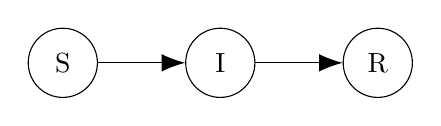
\begin{tikzpicture}[align=center,node distance=2cm and 4cm]
      \node[state] (S) {S};
      \node[state, right of=S] (I) {I};
      \node[state, right of=I] (R) {R};

      \draw (S) edge[-{Latex[length=3mm]}] (I)
            (I) edge[-{Latex[length=3mm]}] (R);
    \end{tikzpicture}
    \caption{Diagram of interactions between compartments in the standard SIR model. S=Susceptible, I=Infectious, R=Removed.}
    \label{fig_sir_model_diagram}
  \end{figure}

  \par These two interactions are governed by a system of three non-linear ordinary differential equations, given in (\ref{eqn_sir_differential_equations}), which represent the change in the total number of individuals in each compartment over time \cite[]{application_of_sir_epidemiological_model}.

  \begin{subequations}\label{eqn_sir_differential_equations}
    \everymath={\displaystyle}\begin{alignat}{2}
      \frac{dS}{dt}&=-\frac\beta{N} S(t)I(t)\label{eqn_sir_differential_equations_S}\\
      \frac{dI}{dt}&=\frac\beta{N} S(t)I(t)-\gamma I(t)\label{eqn_sir_differential_equations_I}\\
      \frac{dR}{dt}&=\gamma I(t)\label{eqn_sir_differential_equations_R}
    \end{alignat}
  \end{subequations}

  \par where $\beta$ is the average number of people infected by the a single infected individual in a single time-period and $\gamma$ is the probability an individual is removed. Initial conditions imposed on this system is that $S(0)\geq0,I(0)\geq0,R(0)\geq0$ and $S(0)+I(0)+R(0)=N$. Note that if $I(t)=0$ at any point in time $t$ then no new infections will occur after time-point $t$. Moreover, if $I(0)=0$ then no infections will ever occur, which is distinctly uninteresting.

  \par In the standard model, $\beta$ and $\gamma$ are non-negative constants with $\beta\in\mathbb{R}^{\geq0},\gamma\in(0,1]$\footnote{$\gamma$ must be non-zero otherwise no-one ever transitions to the removed population and it is impossible for the epidemic to die out.}. Note that $\frac{dS}{dt}+\frac{dI}{dt}+\frac{dR}{dt}=0$ which ensures the total population size is constant and since each differential equation only depends on the current values of $S(t),I(t)$ and $R(t)$, the standard SIR model is Markovian (as all are compartmental models).

  \begin{figure}[H]
    \centering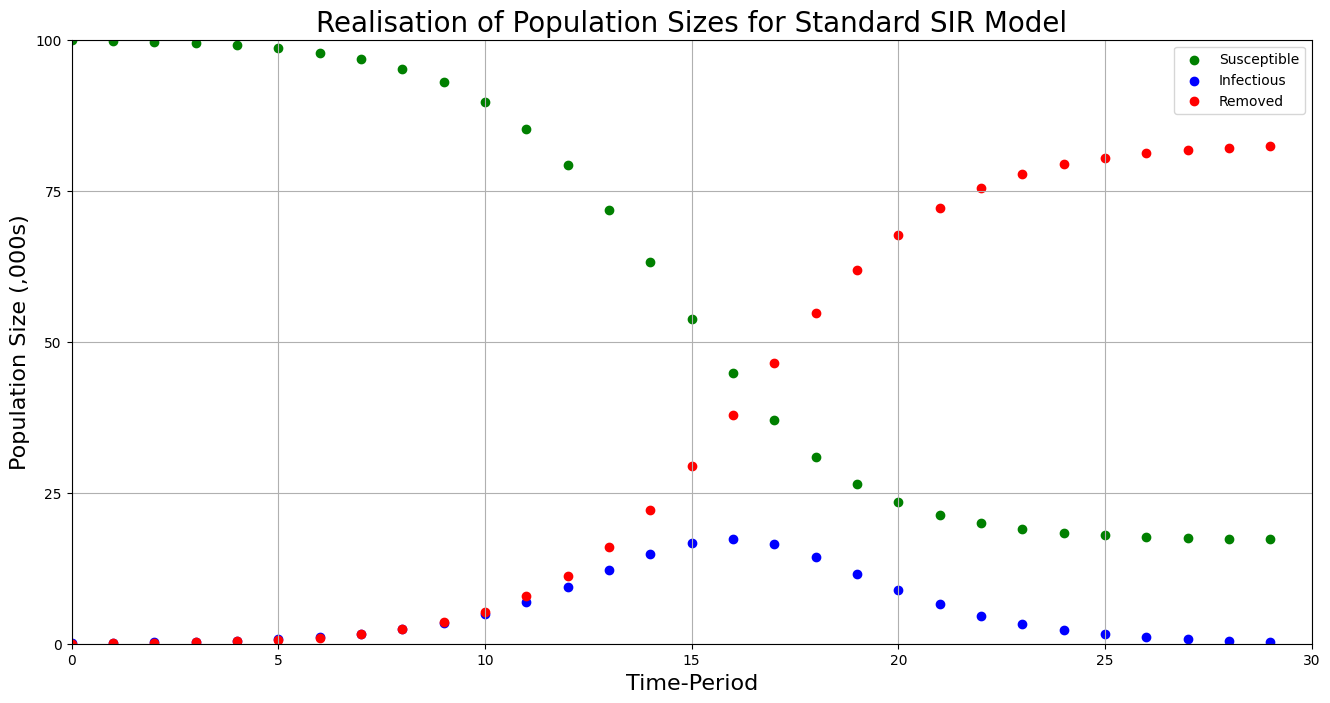
\includegraphics[width=.9\textwidth]{example_sir_model.png}
    \caption{Realisation of a standard SIR model for a population of size $N=100,000$ over 30 time-periods where $\beta=1$ and $\gamma=0.5$. ($R_0=2$)}
    \label{fig_example_standard_sir_model}
  \end{figure}

  \par \textit{Figure \ref{fig_example_standard_sir_model}} provides a plot of how the different compartment sizes vary over time for a standard SIR model for the case where each infected individual passes the disease to one over individual each time-period ($\beta=1$) and there is a 50\% chance an infected individual is removed each time period ($\gamma=0.5$).

  \par In \textit{Figure \ref{fig_example_standard_sir_model}} we can observed that there is a point at which the size of the infectious population begins to decrease. We can mathematically identify this time-point where the gradient $\frac{dI}{dt}$ becomes negative. As $\frac{dI}{dt}=I(t)\left(\frac{\beta S(t)}N-\gamma\right)$ and $I(t)\geq0$ at all time-points $t$, the gradient becomes negative when $\frac{\beta S}N-\gamma<0$. Thus the maximum number of infections occur at time-period $t$ where (\ref{eqn_sir_tipping_point_susceptible}) is satisfied.

  \begin{equation}\label{eqn_sir_tipping_point_susceptible}
    S(t)<\frac{N\gamma}\beta
  \end{equation}

  % TODO can we draw inferences about whether the disease will infect everyone

  \par This result can be written as (\ref{eqn_sir_tipping_point_ir}), in terms of the total population which is either infected or removed. This result is intuitively useful as it provides a value for what proportion of the total population need to be immune from the disease for ``heard-immunity'' to be reached and the rate of spread to decrease naturally. This can be used to set targets for vaccination rollouts. Although the standard SIR model is too basic for these sort of decisions, as it does not allow for $\beta$ or $\gamma$ to vary over time, it is useful for building the intuition which motivates more complex models.

  \begin{alignat}{5}
    &N-&I(t)-R(t)& < &\frac{N\gamma}\beta\nonumber&\\
    \Longleftrightarrow&&N\left(1-\frac\gamma\beta\right)& > &I(t)&+R(t)\label{eqn_sir_tipping_point_ir}
  \end{alignat}

  \par An alterative way to intuitively understand $\beta,\gamma$ is to consider that $1/\beta$ is the mean time between an infected individual infecting someone who is susceptible and $1/\gamma$ is the mean time before an infected individual becomes removed. This means that $\frac{1/\gamma}{1/\beta}$ is the mean number of people each infectious individual infects, assuming all individuals are susceptible. This is the definition of the basic reproduction number $R_0$ and so by simplify we have a simple result for the $R_0$ value of any standard SIR model.

  \begin{equation}
    R_0=\frac\beta\gamma\label{eqn_sir_r0}
  \end{equation}

  \par As $\beta$ and $\gamma$ are constant with respect to time in the standard SIR model, the effective reproduction number $R_t$ is simply the basic reproduction number $R_0$ at all time-points $t$. We can use (\ref{eqn_sir_r0}) to restate the tipping point equation (\ref{eqn_sir_tipping_point_ir}) in terms of the $R_0$ value.

  \begin{equation}
    N\left(1-\frac1{R_0}\right)>I(t)+R(t)
  \end{equation}

  \par Many inference problems focus around the estimation of the parameters $\beta$ and $\gamma$. Given a realisation of the model $\{(S(t),I(t),R(t))\}_t$, it is straightforward to estimate these parameters using the difference equations given in (\ref{eqn_sir_difference_equations}).

  \begin{subequations}\label{eqn_sir_difference_equations}
    \everymath={\displaystyle}\begin{alignat}{2}
      \hat\beta&=\frac{S(t_i)-S_{t_{i+1}}}{S(t_i)I(t_i)}\\
      \hat\gamma&=\frac{R(t_{i+1})-R(t_{i})}{I(t_i)}
    \end{alignat}
  \end{subequations}

  % TODO CLosed form SIR (maybe) (https://ui.adsabs.harvard.edu/abs/2014arXiv1403.2160H) Integral can only be evaluated numerically

  % \par The differential equations which define the standard SIR model are non-integrable in the general case. Finding an exact solution for SIR models is very difficult. \cite[]{note_on_exact_solution_of_sir_and_sis_models} present the first exact solution for a specific case of both an SIR and an SIS model (Discussed later).

\subsection*{SIR Model with Vaccinations}

  \begin{figure}[H]
    \centering
    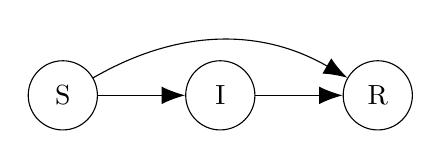
\begin{tikzpicture}[align=center,node distance=2cm and 4cm]
      \node[state] (S) {S};
      \node[state, right of=S] (I) {I};
      \node[state, right of=I] (R) {R};

      \draw (S) edge[-{Latex[length=3mm]}] (I)
            (I) edge[-{Latex[length=3mm]}] (R)
            (S) edge[-{Latex[length=3mm]},bend left=30] (R);
    \end{tikzpicture}
    \caption{Diagram of interactions between compartments in an SIR model with vaccination.}
    \label{fig_sir_model_diagram_w_vaccination}
  \end{figure}

  \par As SIR models are used to model epidemic events, common inferential questions will focus around the effects of introducing a vaccine to a population. For the SIR model it is only necessary to give vaccinations to members of the susceptible population as the removed population are already immune and the infectious population actively have the disease. This means than modelling a vaccination program only requires the inclusion of one extra interaction from the susceptible population to the removed population, as shown in \textit{Figure \ref{fig_sir_model_diagram_w_vaccination}}.

  \begin{subequations}\label{eqn_sir_differential_equations_vaccination}
    \everymath={\displaystyle}\begin{alignat}{2}
      \frac{dS}{dt}&=-\frac\beta{N} S(t)I(t)-\alpha\\
      \frac{dI}{dt}&=\frac\beta{N} S(t)I(t)-\gamma I(t)\\
      \frac{dR}{dt}&=\gamma I(t)+\alpha
    \end{alignat}
  \end{subequations}

  \par Typically this new interaction is implemented by moving a constant number of individuals $\alpha$ from the susceptible population to the removed population. (\ref{eqn_sir_differential_equations_vaccination}) is an extension of (\ref{eqn_sir_differential_equations}) which encodes this interaction. Modelling this as a constant is reasonable for real world scenarios as most vaccination programs aim to vaccinate as many people as possible until the whole susceptible population has been vaccinated, and thus the number of daily vaccinations is very stable. It would be straightforward to define $\alpha(t)$ as a time-dependent function in order to represent an increase in the capacity to vaccinate, or factors such as weekday vs. weekend variations in work patterns.

\subsection*{SIR Model with Demography}

  \par The standard SIR model is very simple and forms a good basis from which to gain intuition for more complex models. A natural advancement is to incorporate births and natural deaths into the model. These processes are known collectively as ``Demography''. It is reasonable to ignore demography for many epidemic processes as the rate of infection and removal from the epidemic process is significantly greater than that from natural demography.

  \par Demography easily extends beyond births and deaths to include immigration and emigration by simply considering immigration and births to be equivalent, and deaths and emigration to be equivalent. If we assume that immigrants cannot carry the disease then these processes are equivalent.

  \par Typically birth is not assumed to bring immunity to diseases, so each birth causes an increase in the size of the susceptible population. Deaths can occur to any individual, regardless of the compartment they are in, and are modelled as completely removing an individual from the population meaning each death leads to a decrease in the total population size. The two interactions from the standard SIR model are unchanged. \textit{Figure \ref{fig_sir_model_diagram_w_demography}} outlines these interactions. This is a good model for diseases, such as chickenpox (VZV), which are endemic in a population but non-fatal.

  \begin{figure}[H]
    \centering
    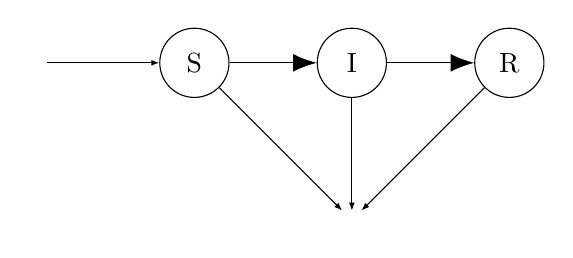
\begin{tikzpicture}[align=center,node distance=2cm and 4cm]
      \node (birth) {};
      \node[state,right of=birth] (S) {S};
      \node[state, right of=S] (I) {I};
      \node[state, right of=I] (R) {R};
      \node[below of=I] (death) {};

      \draw (birth) edge[-{Latex[length=1mm]}] (S)
            (S) edge[-{Latex[length=3mm]}] (I)
            (I) edge[-{Latex[length=3mm]}] (R)
            (S) edge[-{Latex[length=1mm]}] (death)
            (I) edge[-{Latex[length=1mm]}] (death)
            (R) edge[-{Latex[length=1mm]}] (death);
    \end{tikzpicture}
    \caption{Diagram of interactions between compartments in an SIR model with demography.}
    \label{fig_sir_model_diagram_w_demography}
  \end{figure}

  \par Two new parameters are introduced for the encoding of demography: $\lambda$ the number of births per time-period; and $\mu$ the number of natural deaths per time-period. It is assumed that an individual is equally likely to die naturally, regardless of which compartment they are in. The reciprocal of the death rate $1/\mu$ is the average life-span of each individual in the population. Defining $\lambda$ and $\mu$ to be independent of the total population size is reasonable when the overall time-period of the epidemic is relatively short and when recovery from an infection rarely results in death, as the total population is almost constant. The three differential equations (\ref{eqn_sir_w_demography_differential_equations}) model all of these interactions \cite[]{application_of_sir_epidemiological_model}:

  \begin{subequations}\label{eqn_sir_w_demography_differential_equations}
    \begin{alignat}{2}
      \frac{dS}{dt}&=\lambda-\beta S(t)I(t)-\mu S(t)\label{eqn_sir_w_demography_dS_dt}\\
      \frac{dI}{dt}&=\beta S(t)I(t)-\gamma I(t)-\mu I(t)\\
      \frac{dR}{dt}&=\gamma I(t)-\mu R(t)
    \end{alignat}
  \end{subequations}

  where $\beta,\gamma$ are as defined in (\ref{eqn_sir_differential_equations}) and the same initial conditions are imposed.

  \par This system of equations is very similar to (\ref{eqn_sir_differential_equations}) except each equation has a term subtracts the number of natural deaths each time-period, which is proportional to the current population size of the associated compartment. And, (\ref{eqn_sir_w_demography_dS_dt}) has an additional term for introducing natural births.

  \par For the same removal rate $\gamma$, the mean time an individual is infected for is reduced compared to an SIR model without demography due to the possibility of that individual dying naturally before they are removed. The mean time an individual is infected is now $1/(\gamma+\mu)$. This means the $R_0$ for an SIR model with demographics is (\ref{eqn_r0_sir_w_demographics}).

  \begin{equation}\label{eqn_r0_sir_w_demographics}
    R_0=\frac{\beta}{\gamma+\mu}
  \end{equation}

  \par The inclusion of demography in a model allows for two possible equilibria to occur: the disease dies out; or, for the disease to persist in the population as there is a constant influx of new susceptible people. \textit{Remark \ref{rem_equilibria_sir_w_demography}} presents when each of these outcomes occurs and the resulting equilibria. Both the these results hold as time tends to infinity.

  \begin{box_remark}[Equilibria of SIR model with Demography]\label{rem_equilibria_sir_w_demography}
    Note that $\lambda,\beta,\gamma,\mu\geq0$. An equilibrium for the SIR model with demography is achieved when
    \[ \left(\frac{dS}{dt},\frac{dI}{dt},\frac{dR}{dt}\right)=(0,0,0) \]
    There are two cases to consider: $R_0\geq 1$; and, $R_0<1$. For each case, I derive values $(S^*,I^*,R^*)$ for the population sizes which produce an equilibrium.
    \begin{itemize}
      \item[\textit{Case 1}] - $R_0\geq1$.
      \[\begin{array}{rrcl}
        &\frac{dI}{dt}&=&0\\
        \implies&\frac{\beta}N S^*I^*-\gamma I^*-\mu I^*&=&0\\
        \implies&\frac{\beta}N S^*-\gamma-\mu&=&0\\
        \implies&S^*&=&\frac{N(\mu+\gamma)}\beta\\
        &&=&\frac{N}{R_0}\\
        \\
        &\frac{dS}{dt}&=&0\\
        \implies&\lambda-\frac\beta{N} S^*I^*-\mu S^*&=&0\\
        \implies&\lambda-\frac{\beta I^*+\mu N}{R_0}&=&0\\
        \implies&I^*&=&\frac{\lambda R_0-\mu N}\beta\\
        \\
        &\frac{dR}{dt}&=&0\\
        \implies&\gamma I^*-\mu R^*&=&0\\
        \implies&R^*&=&\frac\gamma\mu I^*\\
        &&=&\frac{\gamma\lambda R_0}{\mu\beta}-\frac{\gamma N}\beta
      \end{array}\]
      Thus, when the $R_0\geq1$ an equilibrium is reached when the compartment populations fulfil
      \[ (S,I,R)=\left(\frac{N}{R_0},\ \frac{\lambda R_0-\mu N}\beta,\ \frac{\gamma\lambda R_0}{\mu\beta}-\frac{\gamma N}\beta\right) \]
      This state is known as an ``Endemic Equilibrium'' as the disease maintains a constant level of infection.

      \item[\textit{Case 2}] - $R_0<1$.
      \par As $R_0<1$ the size of the infected population will eventually decrease to zero, after which point no new infections can occur ($I^*=0$). This also means that the removed population can not increase after this point, moreover it will decrease to zero ($R^*=0$) due to those in the population dying. This means the population equilibrium occurs when $\frac{dS}{dt}=0$ and $I=0$.
      \[\begin{array}{rrcll}
        &\frac{dS}{dt}&=&0\\
        \implies&\lambda-\frac\beta{N} S^*I^*-\mu S^*&=&0&\\
        \implies&\lambda-\mu S^*&=&0&\text{ since }I^*=0\\
        \implies&S^*&=&\frac\lambda\mu
      \end{array}\]
      Thus, when the $R_0\geq1$ an equilibrium is reached when the compartment populations fulfil
      \[ (S,I,R)=\left(\frac\lambda\mu,0,0\right) \]
      This state is known as a ``Disease Free Equilibrium''.
    \end{itemize}
  \end{box_remark}

  \begin{figure}[H]
    \centering
    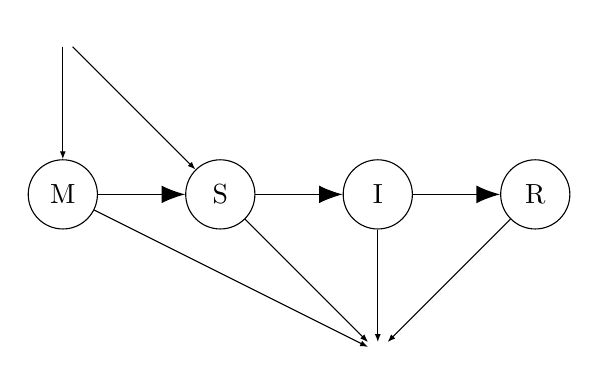
\begin{tikzpicture}[align=center,node distance=2cm and 4cm]
      \node[state] (M) {M};
      \node[above of=M] (birth) {};
      \node[state,right of=M] (S) {S};
      \node[state, right of=S] (I) {I};
      \node[state, right of=I] (R) {R};
      \node[below of=I] (death) {};

      \draw (birth) edge[-{Latex[length=1mm]}] (S)
            (birth) edge[-{Latex[length=1mm]}] (M)
            (M) edge[-{Latex[length=3mm]}] (S)
            (S) edge[-{Latex[length=3mm]}] (I)
            (I) edge[-{Latex[length=3mm]}] (R)
            (M) edge[-{Latex[length=1mm]}] (death)
            (S) edge[-{Latex[length=1mm]}] (death)
            (I) edge[-{Latex[length=1mm]}] (death)
            (R) edge[-{Latex[length=1mm]}] (death);
    \end{tikzpicture}
    \caption{Diagram of interactions between compartments in an MSIR model.}
    \label{fig_msir_model_diagram}
  \end{figure}

  \par For some diseases immunity is passed from mother to child due to antibodies from the mother passing across the placenta. This means that a certain proportion of births are born with immunity, with the proportion typically being the ratio of the size of the removed population to the size of the rest of the population. It would be straightforward to model this by having these children be placed straight into the removed population. However it often makes more sense to create a separate compartment for these children, or to not add these births to the population at all, as many inferential questions focus around the total number of infections.

  \par For some of these diseases, such as measles, the immunity passed from the mother is only temporary and wears off after a period of time. The MSIR\footnote{"Maternal Immunity-Susceptible-Infectious-Removed"} model \cite[]{mathematics_of_infectious_diseases} was introduced to model this scenario, see \textit{Figure \ref{fig_msir_model_diagram}}. The MSIR model introduces a new compartment which is placed before the susceptible compartment, commonly referred to as ``Maternally Derived Immunity'' and denoted by M. A proportion of new births enter the M compartment each time-period, while the rest enter the susceptible population. Members of the M compartment move to the susceptible compartment at a rate $\alpha$, where $1/\alpha$ is the mean time between birth and immunity wearing off, or they die and are removed from the system.

\subsection*{SIR Model with Non-Constant Parameters}

  \par The standard SIR model has limited uses in practice mainly due to its assumptions of constant $\beta$ and $\gamma$, as well as the assumption that all interactions between individuals are equal. These assumptions may be reasonable over short periods of time where there are no changes in the efforts being made to suppress the spread of a disease\footnote{This would likely be due to a disease not being particularly deadly}, such as a single flu season. \cite[]{sir_lecture_slides} fits a standard SIR model to data from the 2004-05 flu season in American and shows how it produces a good fit of the data.

  \par In the real-world true values for the parameters $\beta$ and $\gamma$ do not exist due to noise which occurs from factors such as variability in human interactions, variability in individuals health and the weather. It is much more realistic to model these parameters using non-negative probability distributions and then to sample these distributions each time-period. Due to the removal parameter $\gamma$ needing to be constrained to $(0,1]$ a beta distribution is a common choice. Alternatively, a distribution can be defined for its reciprocal $1/\gamma$ and then $\gamma$ can be calculated after each sample.

  \par Using distributions for model parameters does increase the complexity of analysing such models. However, much of the analysis above can be performed using the expected value of each parameter. Further, the use of distributions allows for further analysis into the uncertainty of a model and whether changes seen are due to changes in policy or just random noise.

\subsection*{SIR Model with Time-Dependent Parameters}

  \par A common modelling problem is to model the effects of introducing a better treatment for those who are infected. This treatment would reduce the mean time each member of the infectious population is infected, and thus an increase to the value of the removal parameter $\gamma$. This is implemented by changing $\gamma$ from being a constant to being a time-dependent step function of the form (\ref{eqn_step_gamma}) where $t'$ is the time-period in which the new treatment is implemented. Naturally, more steps can be added to model several advancements in treatment.

  \begin{equation}\label{eqn_step_gamma}
    \gamma(t)=\begin{cases}
      \gamma_0&t\leq t'\\
      \gamma_1&t>t'
    \end{cases}
  \end{equation}

  \par The same extensions can be made to the infection parameter $\beta$ when seeking to model the affects of public health policies which seek to control the rate of infection.

  \par This concept can be generalised to $\beta(t)$ and $\gamma(t)$ being continuous time-dependent functions to account for other factors such as weather. Implementing such a formulation is practically impossible in practice due to lack of data and the only approximate relationships known between these factors and the nature of the disease.

  \par In (\ref{eqn_sir_differential_equations}) the parameters $\beta$ and $\gamma$ represent very general concepts: the average number of people infected by a single infected individual and the probability of an individual being removed, respectively. And, as such, it is reasonable to consider them as functions of other variables. For example, we could define $\beta$ as (\ref{eqn_alt_beta}) the product of the mean number of interactions an individual has each time-period $b$ and the mean probability of someone becoming infected after an interaction with an infectious individual $c$; And, $\gamma$ as (\ref{eqn_alt_gamma}) the empirical mean for time of an infection across different strains of the disease where \textbf{p} is the distribution of likelihood of each strain and \textbf{s} is the mean time of infection for each strain. The possible formulations are endless. Each formulation introduces more parameters which need to be fitted, increasing the modelling difficulty.

  \begin{subequations}\label{eqn_alt_parameters}
    \begin{alignat}{2}
      \beta&=f(b,c)=b\cdot c\label{eqn_alt_beta}\\
      \gamma&=g(\mathbf{p},\mathbf{s})=\mathbf{p}^T\mathbf{s}\label{eqn_alt_gamma}
    \end{alignat}
  \end{subequations}

  \par Being able to respecify these abstract parameters in terms of real world quantities helps us make a leap from correlation to causation, and to help understand the relative role of different real world events.

\subsubsection{Other Compartmental Models}\label{sec_other_compartmental_models}

  \par The SIR models described so far cover a very narrow, allow common, set of diseases. Here I briefly describe a selection of alternative models to the standard SIR model. To avoid tedium I do not perform much analysis of these models, as it is broadly similar to that of the SIR model for all. It should be apparent that the extensions discussed for the SIR model (demography, vaccinations, maternally derived immunity etc.) are readily applicable to the below models.

  \begin{figure}[H]
    \centering
    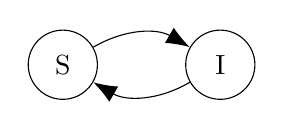
\begin{tikzpicture}[align=center,node distance=2cm and 4cm]
      \node[state] (S) {S};
      \node[state, right of=S] (I) {I};

      \draw (S) edge[-{Latex[length=3mm]},bend left=30] (I)
      (I) edge[-{Latex[length=3mm]},bend left=30] (S);
    \end{tikzpicture}
    \caption{Diagram of interactions between compartments in an SIS model.}
    \label{fig_sis_model_diagram}
  \end{figure}

  \par The SIR model works on the assumption that recovering from an infection confers immunity from future infection of the individual. This is not always the case, especially for diseases with a high mutation rate such as influenza. Once someone has recovered from an infection from one of these diseases they can be returned to the susceptible group. This means the removed group can be removed completely from the model. This is how we reach the SIS\footnote{"Susceptible-Infectious-Susceptible"} model where individuals only move from the susceptible to the infectious group, and back. \textit{Figure \ref{fig_sis_model_diagram}} represents these interactions.


  \par It is straightforward to define differential equations (\ref{eqn_sis_differential_equations}) for the SIS model using those from the standard SIR model (\ref{eqn_sir_differential_equations}). These equations are subject to the restriction that $S(0)\geq0,\ I(0)\geq0$ and $S(0)+I(0)=N$. The $R_0$ value for an SIS model is calculated using the same formula (\ref{eqn_sir_r0}) as for the standard SIR model without demography.

  \begin{subequations}\label{eqn_sis_differential_equations}
    \everymath={\displaystyle}\begin{alignat}{2}
      \frac{dS}{dt}&=\gamma I(t)-\beta S(t)I(t)\\
      \frac{dI}{dt}&=\beta S(t)I(t)-\gamma I(t)\\
    \end{alignat}
  \end{subequations}
  %TODO SIS results (e.g. R0)

  \begin{figure}[H]
    \centering
    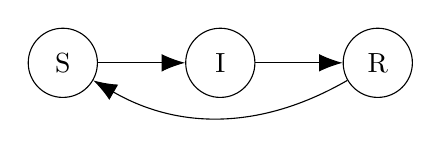
\begin{tikzpicture}[align=center,node distance=2cm and 4cm]
      \node[state] (S) {S};
      \node[state, right of=S] (I) {I};
      \node[state, right of=I] (R) {R};

      \draw (S) edge[-{Latex[length=3mm]}] (I)
      (I) edge[-{Latex[length=3mm]}] (R)
      (R) edge[-{Latex[length=3mm]},bend left=30] (S);
    \end{tikzpicture}
    \caption{Diagram of interactions between compartments in an SIRS model.}
    \label{fig_sirs_model_diagram}
  \end{figure}

  \par A similar class of diseases are those where individuals loose immunity after some period of time. This can be modelled by an extension to the SIR with one additional dynamic as individuals can now move from the removed compartment back to the susceptible compartment. This is formalised as the SIRS\footnote{"Susceptible-Infectious-Removed-Susceptible".} model, see \textit{Figure \ref{fig_sirs_model_diagram}}.

  \begin{figure}[H]
    \centering
    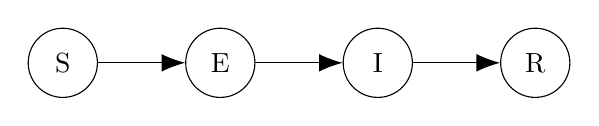
\begin{tikzpicture}[align=center,node distance=2cm and 4cm]
      \node[state] (S) {S};
      \node[state, right of=S] (E) {E};
      \node[state, right of=E] (I) {I};
      \node[state, right of=I] (R) {R};

      \draw (S) edge[-{Latex[length=3mm]}] (E)
            (E) edge[-{Latex[length=3mm]}] (I)
            (I) edge[-{Latex[length=3mm]}] (R);
    \end{tikzpicture}
    \caption{Diagram of interactions between compartments in an SEIR model.}
    \label{fig_seir_model_diagram}
  \end{figure}

  %TODO SEIR
  \par For many diseases an individual does not become infectious to others the moment they become infected with the disease. Rather there is an incubation period where an individual has the disease but cannot yet infect others, and at the end of this period they will become infectious. In the real world this scenario causes problems for epidemiologist and policy makers as it is difficult to ascertain how many people have the disease. A problem which is compounded if individuals are asymptomatic during the incubation period. Alternatively, individuals may be highly symptomatic during the incubation period and thus naturally isolate themselves from the population before they before infectious, heavily reducing the spread of the disease.

  \par The SEIR\footnote{"Susceptible-Exposed-Infectious-Removed"} model is a formalisation of this setup and introduces a new compartment, Exposed (E), between the susceptible and infectious compartments of the standard SIR model.

  % \begin{subequations}\label{eqn_seir_differential_equations}
  %   \everymath={\displaystyle}\begin{alignat}{2}
  %     \frac{dS}{dt}&=-\beta I(t)S(t)\\
  %     \frac{dE}{dt}&=\beta I(t)S(t)-\alpha E(t)\\
  %     \frac{dI}{dt}&=\alpha E(t)-\gamma I(t)\\
  %     \frac{dR}{dt}&=\gamma I(t)
  %   \end{alignat}
  % \end{subequations}

  %TODO SIRD
  \begin{figure}[H]
    \centering
    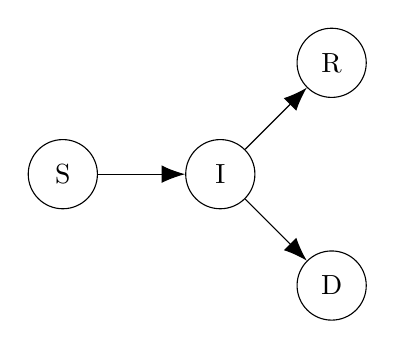
\begin{tikzpicture}[align=center,node distance=2cm and 4cm]
      \node[state] (S) {S};
      \node[state, right of=S] (I) {I};
      \node[state, above right of=I] (R) {R};
      \node[state, below right of=I] (D) {D};

      \draw (S) edge[-{Latex[length=3mm]}] (I)
            (I) edge[-{Latex[length=3mm]}] (R)
            (I) edge[-{Latex[length=3mm]}] (D);
    \end{tikzpicture}
    \caption{Diagram of interactions between compartments in an SIRD model.}
    \label{fig_sird_model_diagram}
  \end{figure}

  % \begin{subequations}\label{eqn_sird_differential_equations}
  %   \everymath={\displaystyle}\begin{alignat}{2}
  %     \frac{dS}{dt}&=-\beta I(t)S(t)\\
  %     \frac{dI}{dt}&=\beta I(t)S(T)-\gamma I(t)-\mu I(t)\\
  %     \frac{dR}{dt}&=\gamma I(t)\\
  %     \frac{dD}{dt}&=\mu I(t)
  %   \end{alignat}
  % \end{subequations}

  \par The final variation of the standard SIR model I will mention is the SIRD\footnote{"Susceptible-Infectious-Removed-Deceased"} model. This model is useful for inferences as it separates the two scenarios by which someone becomes no longer infectious: either becoming removed and thus gaining immunity to future infections; or by dying. This is implemented by adding an additional compartment, deceased (D), to the end of the model and creating a fork which allows for individuals who are infectious to move either the removed or deceased compartments. Different parameters are assigned for each of these dynamics. See \textit{Figure \ref{fig_sird_model_diagram}}

  \par Separating the removed population into these two classes is useful for inferential problems which concern the death rate of a disease. Public health policy makers \underline{should} wish to implement policies which minimise death, and suffering, whilst also minimising the restrictions placed on the lives of individuals.

  \par From these extensions to the standard SIR model, it is evident that the concept of the SIR model can be extended almost endlessly by adding more dynamics and compartments. It is reasonable to want to create different compartments which group people by intrinsic characteristics (age, gender, geography etc.) as it is likely that the parameters governing the dynamics for how each group interacts with a disease will vary. Although these models may better represent a given disease it becomes very difficult to fit them due to their very high degrees of freedom. This is especially true when a population size is relatively small, as the sample size for each compartment will be even smaller and thus random noise will dominate observations. And, these are issues which arise before considering impurity in the available data.

\subsubsection{Stochastic SIR Model}

  \begin{box_definition}[One-Dimensional Brownian Motion\footnote{Also known as a Wiener Process as its existence was proved by Norbert Wiener.}]
    A stochastic process $\{W_t\}_{t\geq0}$ is called Standard Brownian Motion if it fulfils the following for criteria
    \begin{enumerate}
      \item $W_0=0$, almost surely.
      \item Increments of $W$ are independent: $(W_{t+u}-W_t)$ are independent of the filtration $\mathcal{F}_t$ for all $t,u\geq0$.
      \item Increments of $W$ have a stationary Gaussian distributions: $(W_{t+u}-W_t)\sim\mathcal{N}(0,u)$ for all $t,u\geq0$.
      \item $W_t$ is continuous with respect to $t$.
    \end{enumerate}
  \end{box_definition}

  \begin{box_definition}[It\^o Process]
    A stochastic process $\{X(t)\}_{t\in[0,T]}$ is called an It\^o Process if it has the following form
    \[ X(t)=X(0)+\int_0^tb(u,X(u))d_u+\int_0^t\sigma(u,X(u))dW_u \]
    where $b,\sigma$ are functions and $W_t$ is standard one-dimensional Brownian motion. Note that the first integral is a standard integral whilst the second is a stochastic integral.
    \par This form can be stated as the following differential equation
    \[ dX(t)=b(t,X(t))dt+\sigma(t,X(t))dW_t \]
  \end{box_definition}

  \par The SIR model discussed in \textit{Sections \ref{sec_standard_sir_model} \& \ref{sec_other_compartmental_models}} are deterministic\footnote{Disregarding the brief mention of using probability distributions in place of constants.}. This is highly limiting in real-world applications were noise is guaranteed to exist.  \cite[]{infectious_disease_spread_analysis_using_sdes} present a formulation of the SIR model which replaces (\ref{eqn_sir_differential_equations}) with a system of equations which include a stochastic differential equation (\ref{eqn_sir_stochastic_differential_equations}).

  \begin{subequations}\label{eqn_sir_stochastic_differential_equations}
    \begin{alignat}{2}
      dS&=-\frac\beta{N} S(t)I(t)dt\label{eqn_sir_stochastic_differential_equations_S}\\
      dI&=\left(\frac\beta{N} S(t)I(t)-\gamma I(t)\right)dt+\sigma(t,I(t))dW_t\label{eqn_sir_stochastic_differential_equations_I}\\
      R&=N-I(t)-S(t)\label{eqn_sir_stochastic_differential_equations_R}
    \end{alignat}
  \end{subequations}

  where $W_t$ is a one-dimensional Brownian Motion and $\sigma(t,I(t))=\alpha I(t)$ for some diffusion constant $\alpha\in\mathbb{R}$. This system of equations is subject to the initial conditions $I(0)>0$ and $S(0)\geq0$.

  \par The system of equations defined in (\ref{eqn_sir_stochastic_differential_equations}) is very similar to (\ref{eqn_sir_differential_equations}) for the standard SIR model. Moreover, the equations (\ref{eqn_sir_differential_equations_S},\ref{eqn_sir_stochastic_differential_equations_S}) for $\frac{dS}{dt}$ are identical and the definition of (\ref{eqn_sir_stochastic_differential_equations_R}) is necessary to ensure the population size is constant.

  \par The only differences occurs in (\ref{eqn_sir_stochastic_differential_equations_I}) which, due to the inclusion of the stochastic term $\sigma(t,I(t))dW_t$, is now an It\^o Process with $b(t,I(t))=(\beta S(t)I(t)-\gamma I(t))$. This is the equation which turns the system into a stochastic system of equations.

  \par (\ref{eqn_sir_stochastic_differential_equations}) has one additional parameter, the diffusion parameter $\alpha$, which needs to be estimated when compared to (\ref{eqn_sir_differential_equations}). The parameters $\beta$ and $\gamma$ can be estimated using difference equations (\ref{eqn_sir_difference_equations}) as for the standard SIR model. \cite[]{infectious_disease_spread_analysis_using_sdes} recommends the use of (\ref{eqn_estimate_alpha}) as an estimator for the diffusion parameter $\alpha$. This result is follows from the quadratic variance of (\ref{eqn_sir_stochastic_differential_equations_I})

  \begin{equation}\label{eqn_estimate_alpha}
    \hat\alpha^2=\frac{\sum_i\left(I(t_{i+1})-I(t_i)\right)^2}{\sum_i\left(t_{i+1}-t_i\right)I(t_i)^2}
  \end{equation}

  \begin{figure}[H]
    \centering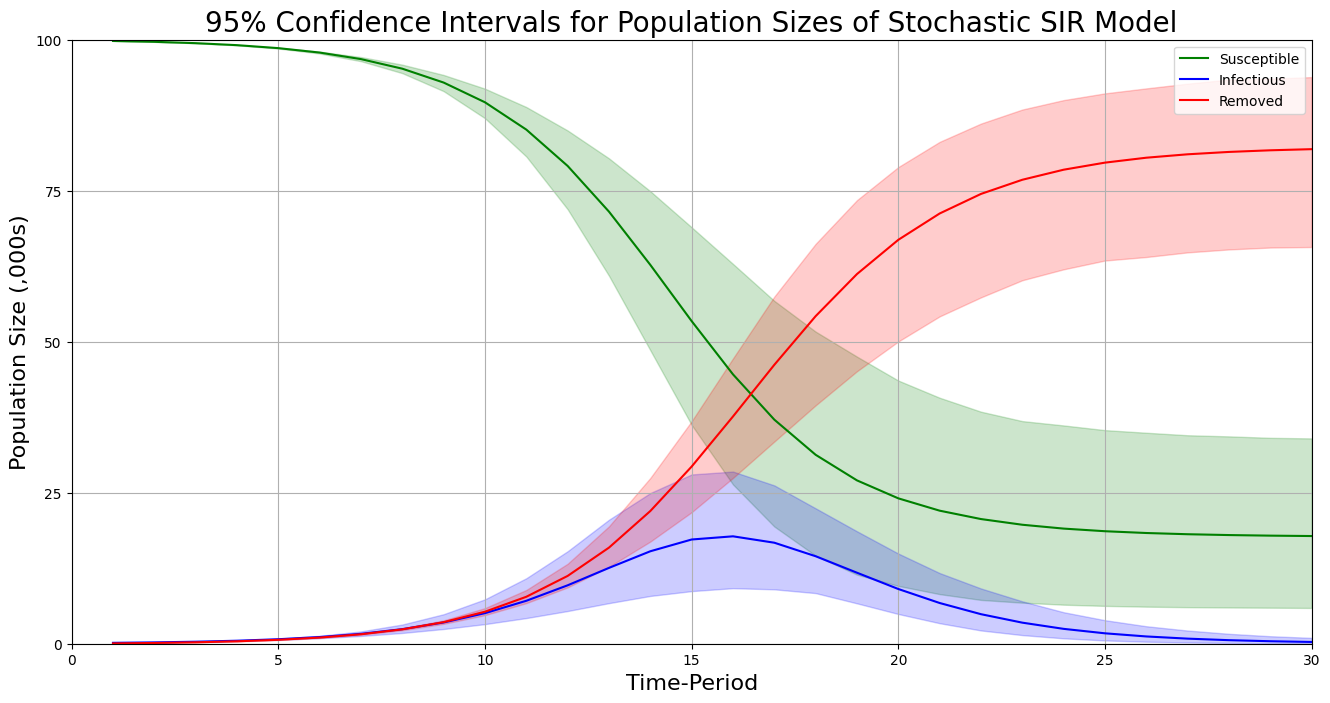
\includegraphics[width=.9\textwidth]{example_stochastic_sir_model.png}
    \caption{95\% confidence intervals for the sizes of the different compartments of a stochastic SIR model with population size $N=100,000$ over 30 time-periods where $\beta=1,\gamma=.0.5$ and $\alpha=0.1$. ($R_0=2$)}
    \label{fig_example_stochastic_sir_model}
  \end{figure}

  \par \textit{Figure \ref{fig_example_stochastic_sir_model}} provides a plot of an example stochastic SIR model. The example model use has the same parameters as the standard SIR model depicted in \textit{Figure \ref{fig_example_standard_sir_model}} except with the diffusion parameter $\alpha=0.1$. Notice how the mean for each series is identical to the realisation in \textit{Figure \ref{fig_example_standard_sir_model}}.

  \par A numerical evaluation of the deterministic system of differential equations (\ref{eqn_sir_difference_equations}) is straightforward as there is only one set of possible results. Whereas, as (\ref{eqn_sir_stochastic_differential_equations}) is stochastic a numerical evaluation is not quite so straightforward. The Euler-Maruyama formula \cite[]{on_one_step_method_of_euler_maruyama} provides a straightforward method for calculating an approximate numerical solution (\ref{eqn_approximate_numerical_stochastic_I}) to a stochastic differential equation such as (\ref{eqn_sir_stochastic_differential_equations_I}).

  \begin{equation}\label{eqn_approximate_numerical_stochastic_I}
    \begin{array}{rrl}
      &I(t_{i+1})&=I(t_i)+\left\{\beta S(t_i)I(t_i)-\gamma I(t_i)\right\}\Delta t_i+\alpha I(t_i)\Delta W_i\\
      \text{where}&\Delta t_i&:=t_{i+1}-t_i\\
      &\Delta W_i&:=W_{t_{i+1}}-W_{t_i}
    \end{array}
  \end{equation}

  \par Note that $\Delta W_i\sim\mathcal{N}(0,t_{i+1}-t_i)$ by the definition of Brownian motion having stationary Gaussian increments, while $\Delta t_i$ can be treated as constant due to it representing a step in time. We can therefore deduce the expectation and variance of $I(t_{i+1})$ given a filtration up to time-period $t_i$ $\mathcal{F}_{t_i}$\footnote{i.e. We know the values of $\{(S(t),I(t),R(T))\}_{t\in[0,t_i]}$.}, as shown below.

  \[\begin{array}{rcl}
    \expect\left[I(t_{i+1})|\mathcal{F}_{t_i}\right]&=&\expect\left[I(t_i)+\left\{\beta S(t_i)I(t_i)-\gamma I(t_i)\right\}\Delta t_i+\alpha I(t_i)\Delta W_i\right]\\
    &=&I(t_i)+\left\{\beta S(t_i)I(t_i)-\gamma I(t_i)\right\}\Delta t_i+\alpha I(t_i)\expect\left[\Delta W_i\right]\\
    &=&I(t_i)+\left\{\beta S(t_i)I(t_i)-\gamma I(t_i)\right\}\Delta t_i\\
    \\
    \var\left[I(t_{i+1})|\mathcal{F}_{t_i}\right]&=&\var\left[\alpha I(t_i)\Delta W_i|\mathcal{F}_{t_i}\right]\\
    &=&(\alpha I(t_i))^2\var[\Delta W_i]\\
    &=&(\alpha I(t_i))^2(t_{i+1}-t_i)\\
  \end{array}\]

  \par By linearity, we can thus deduce the distribution of $I(t_{i+1})$ given a filtration $\mathcal{F}_{t_i}$ to be (\ref{eqn_distribution_I_t_i_plus_1}). This distribution allows us to calculate confidence intervals for the size of the population at each time-period.

  \begin{equation}\label{eqn_distribution_I_t_i_plus_1}
    (I_{t_{i+1}}|\mathcal{F}_{t_i})\sim\mathcal{N}\left(I(t_i)+\left\{\beta S(t_i)I(t_i)-\gamma I(t_i)\right\}\Delta t_i,\ (\alpha I(t_i))^2(t_{i+1}-t_i)\right)
  \end{equation}

  \par This means that the expected result of (\ref{eqn_approximate_numerical_stochastic_I}) is identical to the guaranteed result of (\ref{eqn_sir_differential_equations_I}). This is an important result as it shows (\ref{eqn_sir_stochastic_differential_equations}) describes the same scenarios as (\ref{eqn_sir_differential_equations}) but with stochastic variation. This means much of the analysis performed on the standard deterministic SIR model in \textit{Section \ref{sec_standard_sir_model}} holds for the expected results of the stochastic SIR model discussed hear.

\subsection{Beyond Compartmental Models}

  \par The compartmental models discussed in \textit{Section \ref{sec_other_compartmental_models}} are powerful models when the only population-level data is availble. This data is typically readily available for epidemics; although the accuracy of the data will depend on the reliability and pervasiveness of the testing strategy being used, especially for diseases where infectious people are asymptomatic. In the modern world we now have access to large amounts of individual-level data which concern human behaviours and interactions, namely mobility and personal network data, which are likely useful in modelling an epidemic. It is not obvious how this data could be incorporated in a compartmental model, so we look to other models.

\subsection*{Agent Based Models}
  % \par Agent based models
  % TODO
  % https://ieeexplore.ieee.org/stamp/stamp.jsp?tp=&arnumber=6113095
  % https://www.rips-irsp.com/articles/10.5334/irsp.115/galley/61/download/#:~:text=Limitations%20and%20Drawbacks%20of%20Agent%2DBased%20Models&text=As%20we%20mentioned%20already%20in,practical%20and%20the%20theoretical%20level.
  \par Agent-Based models seek to capture the unique behaviour of each individuals in a population (referred to as ``agents'') by separetly parameterising each individual and specifying a set of rules which define the behaviours of agents. For epidemics, agent-based models  typically have three main components: a model of agent movements; a model of agent-agent interactions; and, a model of the disease which provides a probability of a interaction resulting in an infection (accounting for demographics etc.)

  . There are a number of sources for movement data, one of the most widely used is mobile phone data call/text logs as each event is linked with a cell tower which provides an approximate geographical location. This approach works best in urban areas which cell towers serve smaller areas. The modelling of agent-agent interactions is

  In epidemics, typical agent features include: age, sex, biometrics, medical history, socio-economic status, home address, daily schedule, education level etc.

  \cite[]{agent_based_model_of_epidemic_spread} use cell phone data in an agent-based model to model the 2009 H1N1 outbreak in Mexico and assess the effectiveness of the governments travel restriction policy.

\subsection*{Network Based Models}
  % \par Network based models
  % \par Internet based models

\subsection{Bayesian Modelling of Epidemic Processes}


  \par We have some data (e.g. ....). Now make inferences

  \par A common difficulty in modelling Epidemic Processes is the delay between a public health policy being implemented and the affects of it being seen. % TODO


  % TODO genealise the below 2 paragraphs
  \par Collecting the data required to effectively fit a stochastic SIR model is particulary difficult as, for most disease, only a single epidemic is experienced. This means we often only have a single realisation of the epidemic process and thus calculating variances is very difficult. However, if a disease is experience (effectively) independetly by multiple populations/countries then the data from each of these populations can be considered as an independent realisation of the model once the population sizes have been normalised. If different populations take notably different mitigation strategies then the analysis becomes substanially harder.

  \par A similar approach can be taken for seasonal diseases, such as The Flu, where similar mitigations are taken each year. After normalising for population growth, the data from each year can be considered as an independent realisation of the process.

\newpage
\section{Approximate Bayesian Computation}\label{sec_ABC}

  \par In this section I motivate and provide the mathematical background for Approximate Bayesian Computation (ABC) methods \textit{Section \ref{sec_ABC_background}}; Present the general approach of ABC methods \textit{Section \ref{sec_ABC_ABC_methods}} and discuss four flavours of ABC algorithm \textit{Section \ref{sec_abc_rejection_sampling}-\ref{sec_abc_smc}}; I close this section by exploring how ABC methods can be used for model choice \textit{Section \ref{sec_abc_model_choice}} and how regression adjustment can be used to improve the results of ABC methods \textit{Section \ref{sec_abc_regression_adjustment}}.

\subsection{Motivation and Background}\label{sec_ABC_background}

  % TODO integral can be approximated empirically (https://projecteuclid.org/journals/statistical-science/volume-33/issue-1/Approximate-Bayesian-Computation-and-Simulation-Based-Inference-for-Complex-Stochastic/10.1214/17-STS618.full)

  \par Consider a model $X$ with parameters $\theta$. The centre-point of Bayesian inference is the posterior distribution $\prob(\theta|X)$ for the parameters $\theta$ given observations $X$. Using Bayes rule we have the following formulation for this posterior .

  \[ \prob(\theta|X)=\frac{\prob(X|\theta)\prob(\theta)}{\prob(X)} \]

  \par For Bayesian inference we are only concerned with the relative weight the posterior assigns to each parameter value $\theta$, so we can discard the evidence $\prob(X)$ as it is just a normalising constant with respect to $\theta$. Meaning we can simplify the expression for the posterior as being proportional to the product of the likelihood $\prob(X|\theta)$ and the prior $\prob(\theta)$.

  \[ \prob(\theta|X)\propto\prob(X|\theta)\prob(\theta) \]

  \par As the prior is defined by the user, the only remaining task is to deduce an expression for the likelihood. However, for most real-world processes an explicit expression of the likelihood is computationally intractable due to the complex nature of the systems which govern them and their high degrees of freedom. Moreover, there are often so many parameters that it is intractable to specify all of them and thus we generally theorise a simpler model $\hat{X}$ and seek to calibrate this model to the true model by fitting its parameters. This motivates the need for likelihood-free inference methods such as Approximate Bayesian Computation.

  \begin{center}
    \noindent\rule{.8\textwidth}{0.4pt}
  \end{center}

  \noindent Suppose you have a sequence of $n$ of observations $x_{obs}:=(x_{obs,1},\dots,x_{obs,n})$ from our model $X$ where each observation may be multi-dimensional, $x_{obs,i}\in\mathbb{R}^p$ for $p\in\mathbb{N}$. Let $K_\varepsilon(\cdot)$ denote a kernel density function with bandwidth $\varepsilon>0$ and $\|\cdot\|$ denote a distance measure between observations of model $X$. I discuss kernel density functions and distance measures in \textit{Section \ref{sec_ABC_ABC_methods}}. Note that as the bandwidth tends to zero the value of the kernel density function for the distance between two points $K_\varepsilon(\|x-x_{obs}\|)$ tends to the Dirac delta function $\delta_{x_{obs}}(x)$. This result is trivially from the definition of a kernel density function.

  \begin{equation}
    \lim_{\varepsilon\to0}K_{\varepsilon}(\|x-x_{obs}\|)=\delta_{x_{obs}}(x):=\begin{cases}1&\text{if }x_{obs}=x\\0&\text{otherwise}\end{cases} \label{eqn_limit_of_kernel_and_distance}
  \end{equation}

  \par This result can be used to restate the likelihood function in terms of a kernel density function and distance measure.

  \[
    \everymath={\displaystyle}
    \begin{array}{rcl}
      \prob(x_{obs}|\theta)&=&\int\delta_{x_{obs}}(x)\prob(x|\theta)dx\\
      &=&\lim_{\varepsilon\to0}\int K_\varepsilon(\|x-x_{obs}\|)\prob(x|\theta)dx
    \end{array}
  \]

  \par Consider the following definition $\pi_{ABC}$ and note that it tends to, within a normalising constant, of the true posterior.

  \[
  \everymath={\displaystyle}
  \begin{array}{rrrl}
    &\pi_{ABC}(\theta|x_{obs})&:=&\int K_\varepsilon(\|x-x_{obs}\|)\prob(x|\theta)\pi_0(\theta)dx\\
    \implies&\lim_{\varepsilon\to0}\pi_{ABC}(\theta|x_{obs})&=&\lim_{\varepsilon\to0}\int K_\varepsilon(\|x-x_{obs}\|)\prob(x|\theta)\pi_0(\theta)dx\\
    &&=&\int \delta_{x_{obs}}(x)\prob(x|\theta)dx\cdot \pi_0(\theta)\\
    &&=&\prob(x_{obs}|\theta)\pi_0(\theta)\\
    &&\propto&\prob(\theta|x_{obs})
  \end{array}\]

  \noindent This shows that $\pi_{ABC}$ is an approximation of the true posterior, with it being a good approximation when $\varepsilon$ is small.
  \par Typically, due to the observations $x$ being of high dimension, a summary statistic $s(\cdot)$ is applied to them first and then the quantities $s:=s(x),s_{obs}:=(x_{obs})$ are used in place of $x,x_{obs}$. The analysis of the above derivation is unchanged when using summary statistics as long as the summary statistics are sufficient, if the summary statistics are not sufficient then $\pi_{ABC}$ can only ever be an approximation of the true posterior regardless of the bandwidth used. \textit{Section \ref{sec_summary_stats}} is dedicated to the topic of how to approach choosing summary statistics, with sufficiency being discussed in \textit{Section \ref{sec_sufficiency}}.

  \[ \pi_{ABC}(\theta|s_{obs}):=\int K_\varepsilon(\|s-s_{obs}\|)\prob(s|\theta)\pi_0(\theta)ds \]

  This formulation for the ABC approximation of the posterior is the one found in the standard ABC framework (e.g. \cite[]{overview_of_abc,annual_review_of_statistics_ABC}).

  \par The utility of being able to use $\pi_{ABC}(\theta|s_{obs})$ to approximate the true posterior is apparent when you consider the implied joint distribution of parameters and summary statistics $\pi_{ABC}(\theta,s|s_{obs})$

  \[\everymath={\displaystyle}\begin{array}{rrrl}
    &\pi_{ABC}(\theta|s_{obs})&=&\int \pi_{ABC}(\theta,s|s_{obs})ds\\
    \text{where}&\pi_{ABC}(\theta,s|s_{obs})&:=&K_\varepsilon(\|s-s_{obs}\|)\prob(s|\theta)\pi_0(\theta)
  \end{array}\]

  We can define Monte Carlo algorithms which target sampling from this joint distribution without needing to specify the likelihood $\prob(s|\theta)$. These samples become samples from the posterior by simply ignoring the summary statistic values $s$ which are sampled.

\subsection{ABC Methods}\label{sec_ABC_ABC_methods}

  % TODO state how to estimate posterior density for a given set of summary statistic values $s$ and parameter set $\theta_0$. $\hat\prob(\theta_0|s)=\frac{\sum K'_\zeta(\theta_{i=1}^N-\theta_0)K_\varepsilon(\|s_i-s\|)}{\sum_{i=1}^N K_\varepsilon(\|s_i-s\|)}$ where $K'$ is the function used for kernel density estimation (possibly Epanechnikov) and $\zeta$ is the bandwidth for this kernel.

  \par Approximate Bayesian Computation (ABC) methods are a family computational methods which can be used to approximate posteriors for the parameters of models where the likelihood is intractable. This is achieved by simulating from the likelihood, rather than having to evaluate it explicitly.

  \par The first algorithm to use the concept which would later be known as ABC was presented in \cite[]{inferring_coalescence_times_from_dna_sequence_data}, although this algorithm does not include the use of summary statistics nor use distance measures and kernel density functions to determine whether to accept a simulation or not. The algorithm presented in \cite[]{population_growth_of_human_Y_chromosomes} is much more recognisable as ABC and consider by many as the first true ABC algorithm. This algorithm would later be generalised to becomes the rejection sampling approach to ABC. Both of these papers were studies of population genetics, a field in which ABC is still popular used.

  \par The key feature that simulation based methods exploit is that we only know the response values $x_{obs}$ from the true model, but for each simulation we know the variables values and the response values $(\tilde\theta,\tilde{x})$. Thus we can inspect the parameter values for accepted simulations and draw inferences about the parameter values of the true model. Moreover, it is generally easier to simulate from a model than to reconstruct it

  \par The central concept for all ABC methods is that the likelihood function can be approximated by comparing simulated values to values from a true model. ABC methods require a set of observations from the true model; a theorised model for which parameters can be set and observations generated; and a set of priors for the parameters of the theorised model. ABC methods then perform many simulations of the theorised model and, by comparing  the summary statistic values of the simulated observations to those of the true observations, inferences are made about which parameter values are most likely to be closest to the true values. \textbf{Algorithm \ref{alg_generic_abc}} outlines this basic flow which ABC methods follow. The general idea being that the parameter sets which make the theorised model generate observations which are closest to true observations are more likely to be the true parameter values.

  \begin{box_algorithm}[Generic Approximate Bayesian Computation]\label{alg_generic_abc}
    \textbf{Require:} Observed values $x_{obs}$; Summary statistics $s(\cdot)$; Theorised model $f(X|\cdot)$; Acceptance Kernel $K_\varepsilon(\cdot)$; Distance Measure $\|\cdot\|$.
    \begin{enumerate}
      \item Calculate summary statistic values $s_{obs}=s(x_{obs})$.
      \item Until stopping condition reached:
      \begin{enumerate}
        \item Sample a set of parameters $\tilde\theta$.
        \item Run the theorised model with sampled parameter $\tilde{x}=f\tilde\theta(X|\tilde\theta)$.
        \item Calculate summary statistic values $\tilde{s}=s(\tilde{x})$.
        \item Accepted parameters $\tilde\theta$ with probability $K_\varepsilon(\|\tilde{s}-s_{obs}\|)$.
      \end{enumerate}
      \item Return all accepted parameter sets $\hat\Theta$.
    \end{enumerate}
  \end{box_algorithm}

  \par \textbf{Algorithm \ref{alg_generic_abc}} demonstrates the simplicity of the underlying algorithm for ABC methods. Most ABC methods are straightforward to implement as they follow this basic structure and then change how certain parts of performed in practice (Typically how new samples are drawn and how the acceptance criteria are defined). This allows for a high level of modularity which has motivated innovations in ABC methods.

  \par There are two sources of approximation in the standard ABC algorithm: Use of summary statistics; and, using a bandwidth on the acceptance criteria. The first can be removed by using sufficient summary statistics (See \textit{Section \ref{sec_sufficiency}}). The second is eliminated if the bandwidth is set to zero $\varepsilon=0$ but in general this leads to the algorithms becoming intractable.

  \par The ideal ABC methods are those which run efficiently and perform well with small bandwidths $\varepsilon$. Efficient methods are important as this means more simulations can be processed in a given time-period, making convergence of the estimated posterior more likely. A method being able to handle smaller bandwidths means the posterior it produces will be a better approximation of the true posterior (See Eq. (\ref{eqn_limit_of_kernel_and_distance})). All ABC methods will run with any value of the bandwidth, however those that use an informed search method for generating samples will require fewer simulations to achieve good results (e.g. ABC-SMC).

  \par Monte Carlo methods are a family of algorithms which use repeated random simulations to evaluate a model. These form the basis of how ABC methods approach exploring the parameter space. Monte Carlo methods are a class of methods which seek to generate samples from a space in a way which mimics sampling from the true model. They do this by running many, many simulations and use some degree of randomness to determine how each simulation is generated and which are accepted.

  \par Here is an overview of classes of Monte Carlo methods which are commonly used in ABC methods:
  \begin{itemize}
    \item \textit{Rejection-Sampling methods} calculate a probability $p$ that a given set of simulated values came from the true model. A value $u\sim U[0,1]$ is sampled from standard uniform distribution and if the sampled value $u$ is less than the acceptance-probability $p$ then the simulation is accepted as a sample. This procedure is run on a large number of simulations with each simulation being generated and assessed independently.

    \item \textit{Importance-Sampling methods} extend rejection-sampling by, instead of only accepting a subset of simulated values, all simulations are accepted but each is assigned a weight which indicates the perceived probability that that simulation could be generated by the true model. Typically this weight is the same as the acceptance probability $p$ calculated in rejection-sampling.

    \item \textit{Markov Chain Monte Carlo (MCMC) methods} extend rejection-sampling by, instead of generating each simulation independently, the parameters of the last accepted simulation are slightly perturbed and then used to generate a new simulation. This creates a search process rather than random simulation due to the dependency between consecutive samples.

    \item \textit{Sequential Monte Carlo (SMC) methods}\footnote{Also known as Particle-Filter methods.} extend importance-sampling by repeatedly resampling from the set of samples, with the weights of each parameter determining the probability it is sampled, and each iteration tightening the acceptance criteria. This means the estimated posterior will become more refined each time and hopefully converge on the true posterior.
  \end{itemize}

  \par The use of Monte Carlo methods means that ABC methods are inherently computationally inefficient due to the need to perform many random simulations. This inefficiency means ABC methods perform badly for models which generate a lot of data as it takes longer to assess each simulation. In the most extreme cases part of this data needs to be omitted for computational efficiency which naturally adds another layer of approximation. Being able to increase the acceptance rate of simulations means less simulations are required and thus more complex models can be assessed. ABC-MCMC generally achieves the greatest acceptance rates for a given bandwidth.

  \par Monte Carlo methods introduce a high degree of randomness into ABC methods which further motivates the need to perform lots of simulations as the strong law of large number is required to obtain consistent results. This limitation is mitigated due to the simplicity of most ABC algorithms meaning they are capable of process millions of simulations an hour on modern computers.

  \par The set of accepted parameter sets $\hat\Theta$ returned by ABC can be used for Bayesian inference. Estimating properties of the distributions, such as mean, mode and quantiles, is straightforward. Producing a discretised estimate of the posterior for each parameter can be achieved by calculating a histogram of the accepted values for each parameter, again straightforward. Kernel density functions can be used to produce a continuous estimates of the posteriors (See \cite[]{review_of_kde}).

  \begin{box_remark}[Posterior Mean is Minimum Mean-Square Error Estimator]\label{rem_posterior_mean_is_mmsee}
    Let $\theta$ denote the quantity we wish to estimate, $A$ denote an arbitrary estimator of $\theta$ and suppose we have observed $x_{obs}$ from model $X$. Then
    \[\begin{array}{rrcl}
      &MSE_\theta(A)&=&\expect\left[(\theta-A)^2|X=x_{obs}\right]\\
      &&=&\expect\left[\theta^2-2A\theta+A^2|X=x_{obs}\right]\\
      &&=&\expect\left[\theta^2|X=x_{obs}\right]-2A\expect\left[\theta|X=x_{obs}\right]+A^2\\
      \implies&\frac{\partial}{\partial A}MSE_\theta(A)&=&-2\expect[\theta|X=x_{obs}]+2a\\
      \implies&a&=&\expect[\theta|X=x_{obs}]
    \end{array}\]
    This shows that mean-square error is minimised when the posterior mean of $\theta$ given $x_{obs}$ is used as an estimator.
  \end{box_remark}

  \par ABC methods are commonly used to calibrate models or to compare models. Typically calibration is done by setting parameter values to the estimated posterior mean as the posterior mean minimises mean-square error (see \textbf{Remark \ref{rem_posterior_mean_is_mmsee}}). ABC methods are used for model comparison as they can directly estimate Bayes factor, I discuss model comparison further in \textit{Section \ref{sec_abc_model_choice}}.

  \par The key advantage of ABC methods, over other approaches to Bayesian inference, is that it produces a distribution, rather than a point-estimate, for parameter values. This allows for analysis into uncertainty around the parameter values. Additionally, as the strictness of the acceptance criteria is a parameter of ABC methods, ABC methods can fit or compare a large range of theorised models by loosening the acceptance criteria. Being able to use simpler models has the advantage of reducing issues which occur due to curse-of-dimensionality.

  \par A limitation of using ABC methods is the large number of hyper-parameters they have (Distance measures, summary statistics, bandwidths, perturbation kernels, etc.) and that the choices the user makes for how these parameters are set can drastically affect the algorithms performance. It is trivial to realise that if an uninformative distance measure such as $\|x\|=0\ \forall\ x$ is used or an acceptance kernel which accepts all simulations is used then the returned set of parameters will resemble the set of priors, and no meaningful inferences can be drawn. Moreover, these hyper-parameters need to be tuned for each model these methods are applied, which is laborious. This has motivated the innovation of adaptable ABC algorithms which automate the process of setting some of these parameters.

  \par As stochastic processes determine whether a simulation is accepted, or not, ABC methods incur information loss. This can mean that promising areas of the parameter space are not explored. This issue is mitigate by running many simulations.

  % TODO trade-off of low v high bandwidth (time v accuracy basically) no obvious relationship between the two

\subsubsection*{Summary Statistics}

  \par See \textit{Section \ref{sec_summary_stats}}.

\subsubsection*{Kernel Density Functions}

  \begin{box_definition}[Kernel Density Functions $K_\varepsilon(\cdot)$, \cite{non_parameteric_estimation_of_a_multivariate_probability_density}]
    Kernel density functions are functions $K:\mathbb{R}\to\mathbb{R}$ with the following properties:
    \begin{enumerate}
      \item Non-negative
      \[ K_\varepsilon(x)\geq0\ \forall\ x\in\mathcal{X} \]
      where $\mathcal{X}$ is the range of values $x$ can take.
      \item Symmetric
      \[ K_\varepsilon(x)=K_\varepsilon(-x)\ \forall\ x\in\mathcal{X} \]
      \item Normalised
      \[ \int_{\mathcal{X}}K_\varepsilon(x)dx=1 \]
      \item $K_\varepsilon(x)=\frac1\varepsilon K_1(x/\varepsilon)$.
    \end{enumerate}
    \noindent Kernel density functions are typically extended to allow for a smoothing parameter $\varepsilon\geq0$ such that $K_\varepsilon(x)=\frac1\varepsilon K(x/\varepsilon)$.
  \end{box_definition}

  \par The choice of kernel density function does not play a notable role in the asymptotic behaviour of ABC methods, however the bandwidth chosen for them does. A high bandwidth means that the weight of the kernel is spread much more evenly across its support meaning there is less discrimination between values close to the mean and those further away.

  \par It is standard to define kernel density functions such that they have zero mean. Having this property means that that $\max_xK_\varepsilon(x)=K_\varepsilon(0)$, this follows immediately from the kernel being symmetric. This is a useful property in the context of ABC methods as we pass the distance between two points $\|x-x_{obs}\|$ to the kernel density function to determine the probability we accept a simulation and this property means that simulations $x$ closest to the observed values $x_{obs}$ are more likely to be accepted.

  \par In practice, when implementing ABC methods we typically scale up the values returned by the kernel such that $K_\varepsilon(0)=1$. This is straightforward to do for well-known kernels as it only requires the removal of the normalising term. As the relative weights given to each value are maintained this does not affect the asymptotic behaviour of the algorithms, but will increase the acceptance rate. This also has the desirable effect that every time an exact match is found it will definitely be accepted.

  \begin{table}[H]
    \everymath={\displaystyle}
    \centering
    \begin{tabular}{|l|l|}
      \hline
      \textbf{Name}&\textbf{Formula}\\\hline
      Uniform Kernel&$K_\varepsilon(x)=\frac1{2\varepsilon}\mathbbm{1}\{x\leq\varepsilon\}$\\\hline
      Gaussian Kernel&$K_\varepsilon(x)=\frac\varepsilon{\sqrt{2\pi}}\exp\left\{-\frac12x^2\varepsilon^2\right\}$\\\hline
      Epanechnikov Kernel&$K_\varepsilon(x)=\frac34\left(1-x^2\varepsilon^2\right)\mathbbm{1}\left\{|x|\leq\varepsilon\right\}$\\
      \hline
    \end{tabular}
    \caption{Common kernel density functions for ABC methods.\protect\footnotemark}
    \label{tab_common_kernels}
  \end{table}
  \footnotetext{$\mathbbm{1}\{A\}:=\begin{cases}1&\text{if }A\\0&\text{otherwise}\end{cases}$}

  \par \textbf{Table \ref{tab_common_kernels}} provides a table of the most commonly used kernel density functions for ABC, as recommended by \cite[]{annual_review_of_statistics_ABC}. The Epanechnikov kernel is asymptotically optimal for kernel density estimation when seeking to minimise mean-square error (See \cite[]{non_parameteric_estimation_of_a_multivariate_probability_density}), although this theoretical result is disputed in \cite[]{introduction_to_nonparametric_estimation}.

  \par The uniform kernel is popular in ABC as it is equivalent to accepting all simulations whose distance from the true observation is no greater than $\varepsilon$. This creates spherical acceptance regions when using the Euclidean distance or rectangular ones when using Manhattan distance. The Gaussian kernel is more commonly used as it has an infinite support which is useful in certain scenarios. When choosing which kernel to use for ABC methods it is intuitive that it should match the theorised distribution of the noise in the theorised model. This further motivates the popularity of a gaussian kernel as many models assume gaussian noise.

\subsubsection*{Distance Measures}\label{sec_distance_measures}

  \begin{table}[H]
    \everymath={\displaystyle}
    \centering
    \begin{tabular}{|l|l|}
      \hline
      \textbf{Name}&\textbf{Formula}\\\hline
      Manhattan Distance&$L_1(\mathbf{x}):=\sum_{i=1}^m|x_i|$\\\hline
      Euclidean Distance&$L_2(\mathbf{x}):=\sqrt{\sum_{i=1}^mx_i^2}$\\\hline
      $L_p$ Norm&$L_p(\cdot):=\left(\sum_{i=1}^mx_i^p\right)^{1/p}$\\\hline
      $L_\infty$ Norm&$L_\infty(\mathbf{x}):=\max\{x\in \mathbf{x}\}$\\\hline
    \end{tabular}
    \caption{Common distance measures for ABC methods.}
    \label{tab_common_distances}
  \end{table}

  \par Distance measures quantify how far apart two multi-dimensional vectors are from each other, with greater values indicating the vectors are further away. A value of zero means that the two vectors are identical under the given measure.

  \par The choice of distance measure is integral to the performance of an ABC method as it determines whether a set of simulated values are deemed to be representative of the true model, or not, by quantifying how similar these values are to true observations. \textbf{Table \ref{tab_common_distances}} provides a list of popular distance measures for ABC methods. The Euclidean distance is most commonly as minimising Euclidean distance is clearly related to minimise SSE of a model.

  \par It is important to note that the value passed to distances measures in ABC methods is the difference of two sets of summary statistics. Well chosen summary statistics will extract meaningful information and perform a certain level of pre-processing of this data such as standardisation and weighting different dimensions. This means we do not need to consider these problems during selection of distance measure.

  \par An issue which arises when specifying distance measures is the ``Curse of Dimensionality''\footnote{Term first coined in \cite[]{adaptive_control_processes} in reference to how many algorithms may work well when applied to low-dimensions, but are intractabled when for higher-dimensions.}. This is the phenomena that as the dimensionality of vectors being compared increases, it becomes harder to distinguish between different pairs. This is an issue to ABC methods as the success of the approach relies on being able to accurately identify which simulations are closest to observed values. Using summary statistics which introduce a high level of dimensionality reduction will help.

  \par Different demonstrations of this phemonema is required for different distance measures, but for Euclidean distance it is generally demonstrated by comparing of the volume of a hyper-sphere with radius $r$ and the volume of a hyper-cube with side length $2r$. The volume of the hyper-cube quickly dwarfs that of the hyper-sphere as the number of dimensions are increased. % TODO incude mathematical proof (https://en.wikipedia.org/wiki/Curse_of_dimensionality#Distance_functions)
  The ``Curse of Dimensionality'' is a big short coming of the Euclidean distance as it was only every conceived for real-world spaces (i.e. two or three dimensions). Which distance measure is best ultimately depends on the data being used. Using the $L_p$ norm has shown promise but adds the additional problem of what value of $p$ is optimal. \cite[]{choosing_the_metric_in_high_dimensional_spaces_based_on_hub_analysis} present an approach to choosing an optimal $p$ which assesses the ``hub-ness'' of a dataset.

  \par There is a wealth of literature on the ``Curse of Dimensionality'' in the machine learning space, particularly for nearest-neighbour problems which are very relevant to the problem being addressed by distance measures in ABC (See \cite[]{when_is_nearest_neighbour_meaningful,what_is_the_nearest_neigbour_in_high_dimensional_space,hubs_in_space})

\subsubsection{ABC-Rejection Sampling}\label{sec_abc_rejection_sampling}

  % TODO justify validity of generic rejection samplers

  ABC-Rejection Sampling is a generalisation of the sampling algorithms presented in \cite[]{inferring_coalescence_times_from_dna_sequence_data,population_growth_of_human_Y_chromosomes}. The general idea is to keep simulating from the theorised model until a predefined number of simulations $M$ have been accepted by the acceptance kernel. Each simulation involves sampling a set of parameters $\tilde\theta$ from the predefined priors $\pi_0(\theta)$; initialising the theorised model $f(X|\theta)$ with the sampled parameters; Observing values $\tilde{x}$ from the initialised model and then comparing these observations to observations from the true model using summary statistics $s$, a distance measure $\|\cdot\|$ and a acceptance kernel $K_\varepsilon(\cdot)$. This approach is stated formally in \textbf{Algorithm \ref{alg_abc_rejection_fixed}}.

  \par ABC-rejection sampling is most suitable in problems where it is believed that the posterior is not very different from the defined priors, as this algorithm has very limited search capabilities. These are typically problems which have already been studied heavily an a general understanding of the priors is known.

  \begin{box_algorithm}[ABC-Rejection Sampling ``Fixed Sample Size'']\label{alg_abc_rejection_fixed}
    Adapted from \cite[]{ABC_in_population_genetics}.
    \par
    \begin{algorithm}[H]
      \SetKwIF{With}{}{Else}{with probability}{}{}{otherwise}{}
      \SetKwInOut{Require}{require}
      \Require{Observed values $x_{obs}$; Summary statistics $s(\cdot)$; Theorised model $f(X|\cdot)$; Prior Distributions $\pi_0(\theta)$; Acceptance Kernel $K_\varepsilon(\cdot)$; Distance Measure $\|\cdot\|$; Target Number $M$.}
      $s_{obs}\leftarrow s(x_{obs})$.\\
      $\tilde\Theta\leftarrow\{\}$.\\
      $t\leftarrow0$.\\
      \While{$t<M$}{
        $\tilde\theta_t\leftarrow$ sample $\pi_0(\theta)$.\\
        $\tilde{x}\leftarrow f(X|\tilde\theta_t)$.\\
        $\tilde{s}\leftarrow s\left(\tilde{x}\right)$.\\
        \With{$K_\varepsilon(\|s_{obs}-\tilde{s}\|)$} {
          $\hat\theta^{(t)}\leftarrow\tilde\theta$.\\
          Add $\hat\theta^{t}$ to $\hat\theta$.\\
          $t\leftarrow t+1$
        } \lElse {Pass}
      }
      \Return{$\tilde\Theta=\left\{\theta^{(1)},\dots,\theta^{(M)}\right\}$}
    \end{algorithm}
  \end{box_algorithm}

  \par The approach in \textbf{Algorithm \ref{alg_abc_rejection_fixed}} is intuitive and simple to implement. A limitation of this simplicity is that each simulation is completely independent and no ``learning'' is incorporated from information about which parameter sets have previously been accepted, or rejected. However, this independence does mean that it is straight forward to implement \textbf{Algorithm \ref{alg_abc_rejection_fixed}} in a parellisable fashion, allowing for more simulations to be analysed in a given time-period.

  \par A practical difficulty in using \textbf{Algorithm \ref{alg_abc_rejection_fixed}} is in setting the bandwidth of the acceptance kernel as the bandwidth dictates the acceptance rate $\lambda$. A lower acceptance rate means more meaningful inferences can be drawn from the results as the average distance between accepted simulations and the true observations will be lower, and thus the accepted simulations will be more informative. However, there is no clear relationship between bandwidth and the acceptance rate of the algorithm so run-times are near-impossible to predict to any meaningful degree of accuracy.

  \begin{box_algorithm}[ABC-Rejection Sampling ``Best Samples'']\label{alg_abc_rejection_best}
    \begin{algorithm}[H]
      \SetKwInOut{Require}{require}
      \Require{Observed values $x_{obs}$; Summary statistics $s(\cdot)$; Theorised model $f(X|\cdot)$; Prior Distributions $\pi_0(\theta)$ Distance Measure $\|\cdot\|$; Number of Simulations $M$; Simulations to Accepted $N$.}
      $s_{obs}\leftarrow s(x_{obs})$.\\
      $\tilde\Theta\leftarrow\{\}$.\\
      $t\leftarrow0$.\\
      \For{$i=0,\dots,M$}{
        $\tilde\theta^{(i)}\leftarrow$ sample $\pi_0(\theta)$.\\
        $\tilde{x}^{(i)}\leftarrow f(X|\tilde\theta^{(i)})$.\\
        $\tilde{s}^{(i)}\leftarrow s\left(\tilde{x}^{(i)}\right)$.\\
        $d^{(i)}\leftarrow\|s(\tilde{x}^{(i)})-s_{obs}\|$.\\
        Add $(d^{(i)},\tilde\theta^{(i)})$ to $\tilde\Theta$.
      }
      \Return{$N$ elements with smallest distance values $d^{(i)}$.}
    \end{algorithm}
  \end{box_algorithm}

  \par The problem of setting a bandwidth (and acceptance kernel) can be avoid completely by instead running a fixed number $M$ of simulations and then accepting a predefined number $N$ of these which are closest to the observed values, effectively defining the acceptance rate. Additionally, this removes the risk of the algorithm running indefinitely. This approach is outlined in \textbf{Algorithm \ref{alg_abc_rejection_best}}. This algorithm runs in linear time with-respect-to the number of simulations $O(M)$, as the set of simulated values $\tilde\Theta$ is unsorted with-respect-to the distance values $d^{(i)}$ and thus finding the $N^{th}$ order-statistic takes linear time.

  \par The space requirements for \textbf{Algorithm \ref{alg_abc_rejection_best}} grow linearly with-respect-to the number of simulations being run $O(M)$. This creates a pratical limit of the number of simulations which can be run. The space requirements can be reduced to $O(N)$ (grow linearly wrt the number of accepted simulations) by, instead of storing all simulations in the set $\tilde\Theta$, we instead only store the $N$ closest. This requires keeping the set $\tilde\Theta$ ordered and thus increases the time complexity of the algorithm to $O(M\log_2 N)$.

  \par There is no requirement for the number of simulations, nor the number to accept, to be defined for running the algorithm. Rather the algorithm can be allowed to run and assess simulations until a time limit is reached. Then either a predefined proportion of the simulations can be accepted, or the distribution of distances can be inspected to choose an acceptance rate. The disadvantage of this approach is that it has high space requirements due to the need to store the distance and parameters for all simulations until the very end of the algorithm. This creates a cap on how long this version of the algorithm could be run, but this can be mitigated by dropping the very worst simulations (among other approaches).

  \par The set of accepted simulations returned by ABC-Rejection Sampling techniques places an equal weighting on each simulation. A natural extension is to place greater weight on parameters which produce values which are closer to those produced by the true model. \cite[]{ABC_in_population_genetics} propose a technique of weighted local-linear regression to adjust parameter values where the weights are determined by the distance value associated with the parameter set.

  \par Rejection sampling techniques can be used to estimate the probability of a given set of results under different models $f(X|M)$. This is useful in model choice as it immediately leads to estimations of Bayes' factor. I discuss this further in \textit{Section \ref{sec_abc_model_choice}}.

\subsubsection{ABC-Importance Sampling}\label{sec_abc_importance_sampling}

  % NOTE https://bookdown.org/rdpeng/advstatcomp/importance-sampling.html

  \par Importance sampling methods use a tractable distribution to sample from an intractable distribution. Importance sampling is an exact method as, given enough iterations, it will always converge on target distribution in an unbiased fashion. The theory behind importance sampling is laid out in \textbf{Remark \ref{rem_importance_sampling}}.

  \begin{box_remark}[Importance Sampling]\label{rem_importance_sampling}
    Let $X$ be a model $X\sim h(X;\theta)$ with parameters $\theta$. Consider two distributions for parameter values $f(\theta),g(\theta)$ where $f$ is a target distribution, from which sampling is intractable, and $g$ is a distribution we can sample from. Then the expected value of $X$ under distribution $f$ is the same as the expected value of $X\cdot w(\theta)$ under distribution $g$, where $w(\theta):=\frac{f(\theta)}{g(\theta)}$ is a weight measure.
    \everymath={\displaystyle}
    \[\begin{array}{rcl}
      \expect_f[X]&=&\int h(X;\theta)f(\theta)d\theta\\
      &=&\int h(X;\theta)f(\theta)\frac{g(\theta)}{g(\theta)}d\theta\\
      &=&\int h(X;\theta)g(\theta)\frac{f(\theta)}{g(\theta)}d\theta\\
      &=&\int h(X;\theta)g(\theta)w(\theta)d\theta\text{ where }w(\theta):=\frac{f(\theta)}{g(\theta)}\\
      &=&\expect_g[h(X;\theta)w(\theta)]
    \end{array}\]
    This means we can estimate the expected value of the model under $f$ by weighting samples from $g$ using $w(\theta)$. This is the likelihood ratio of an observation coming from the two models.
  \end{box_remark}

  \par In ABC context the target distribution is the approximate joint distribution posterior $f=\pi_{ABC}(\theta,s|s_{obs})$ and the distribution we can sample from is the joint distribution of summary statistics and parameters under the importance distribution $g(s,\theta)=p(s|\theta)g(\theta)$. The importance weighting $\tilde{w}$ for each simulation in ABC is derived below.

  \[\everymath={\displaystyle}\begin{array}{rcl}
    \frac{\pi_{ABC}(\theta,s|s_{obs})}{g(\theta,s)}&\propto&\frac{K_\varepsilon\left(\|s-s_{obs}\|\right)p(s|\theta)\pi_0(\theta)}{p(s|\theta)g(\theta)}\\
    &=&\frac{K_\varepsilon\left(\|s-s_{obs}\|\right)\pi_0(\theta)}{g(\theta)}\\
    &=:&\tilde{w}
  \end{array}\]

  \par ABC-Importance Sampling should be used in cases where we have a good idea of what the distribution for the posterior will be so that the prior $\pi_0$ and importance distribution $g$ are informative.

  \par An importance sampling approach to ABC is an extension of the rejection sampling approach which replaces calculating acceptance probabilities with calculating importance weightings to each simulation. All simulations are accepted and their importance weight is used to weight them during Bayesian inference. An acceptance kernel $K_\varepsilon$ and distance measure $\|\cdot\|$ still need to be specified as they are required to calculate the importance weights. This approach is given in \textbf{Algorithm \ref{alg_abc_importance_sampling}}.

  \begin{box_algorithm}[ABC-Importance Sampling]\label{alg_abc_importance_sampling}
    Adapted from \cite[]{abc_samplers}.
    \par
    \begin{algorithm}[H]
      \SetKwInOut{Require}{require}
      \Require{Observed values $x_{obs}$; Summary statistics $s(\cdot)$; Theorised model $f(X|\cdot)$; Prior Distributions $\pi_0(\theta)$ Distance Measure $\|\cdot\|$; Number of Simulations $M$; Importance Kernel $g(\cdot)$.}
      $s_{obs}\leftarrow s(x_{obs})$.\\
      $\tilde\Theta\leftarrow\{\}$.\\
      \For{$i=0,\dots,M$}{
        $\tilde\theta^{(i)}\leftarrow$ sample $g(\theta)$.\\
        $\tilde{x}^{(i)}\leftarrow f(X|\tilde\theta^{(i)})$.\\
        $\tilde{s}^{(i)}\leftarrow s\left(\tilde{x}^{(i)}\right)$.\\
        $\tilde{w}^{(i)}\leftarrow \frac{\pi_0\left(\theta^{(i)}\right)}{g\left(\theta^{(i)}\right)}K_\varepsilon\left(\left\|s^{(i)}-s_{obs}\right\|\right)$.\\
        Add $\tilde\theta^{(i)}$ to $\tilde\Theta$ with weight $\tilde{w}^{(i)}$.\label{alg_abc_is_accept}
      }
      \Return{$\tilde\Theta:=\left\{\left(\tilde\theta^{(1)},\tilde{w}^{(1)}\right),\dots,\left(\tilde\theta^{(M)},\tilde{w}^{(M)}\right)\right\}$}
    \end{algorithm}
  \end{box_algorithm}

  \par Similar to ABC-Rejection Sampling, \textbf{Algorithm \ref{alg_abc_importance_sampling}} is straightforward to implement in a parallelisable fashion due to the independence of each simulation. However, it is much less space efficient than the ABC-Rejection Sampling approaches as it requires the storage of every simulation. This is mitigated by an approach presented by \cite[]{constructing_summary_statistics_for_approximate_bayesian_computation_semi_automatic_ABC} which combines the rejection and importance sampling approaches to ABC. I discuss this approach more further down.

  \par The approach to ABC-Importance Sampling given in \textbf{Algorithm \ref{alg_abc_importance_sampling}} requires the specification of priors $\pi_0(\theta)$ and an importance distribution $g(\theta)$. If these distributions are the same, or proportional to each other, then $\frac{\pi_0(\theta)}{g(\theta)}\approx 1\ \forall\ \theta$ meaning the acceptance probability $K_\varepsilon(\|s-s_{obs}\|)$ is the only factor weighting each simulation.

  \par An issue with all sampling approaches which weight their results is that it is possible for a small subset of accepted samples to dominate the weight space. This can lead to results becoming unstable. This can naturally be tackled by increasing the number of simulations, this is inefficient and does not inform us as to when a sufficient number of simulations have been made. The Effective Sample Size ($ESS$) is a useful metric in these cases as it quantifies how many equally weighted samples our set is equivalent to. The stopping condition of the algorithm should be updated such that the algorithm terminates once the effective sample size of the accepted set of parameters has reached some threshold $N$
  \[ ESS:=\frac{\sum_{i=0}^M w^{(i)}}{\sum_{i=0}^M \left(w^{(i)}\right)^2} \]
  where $(w^{(0)},\dots,w^{(M)})$ is the weights assigned to each simulation.

  \par \cite[]{constructing_summary_statistics_for_approximate_bayesian_computation_semi_automatic_ABC} propose an algorithm which combines ABC-Rejection Sampling and ABC-Importance Sampling by, rather than accepting every simulation (Line \ref{alg_abc_is_accept}), each simulation is accepted with probability $K_\varepsilon(\|s-s_{obs}\|)$ and is assigned weight $\tilde{w}=\pi_0(\theta)/g(\theta)$. This reduces the accepted set of simulations to only those that produce reasonably similar responses, compared to the true model. This improves the effective sample size of the set of accepted parameters as fewer simulations are given very small weights, and is more space efficient that \textbf{Algorithm \ref{alg_abc_importance_sampling}} as it does not require every simulation to be stored.

\subsubsection{ABC-MCMC}\label{sec_abc_mcmc}

  \begin{box_definition}[Markov Chain]
    A Markov Chain is a Stochastic Process $\{X_t\}_{t}$ with the Markov Property. This means that the current state of the process solely depends on its state in the time-period immediately before.
    \[ \prob(X_{t+1}|X_t,\dots,X_1)=\prob(X_{t+1}|X_t) \]
    \par The transitions a Markov Chain can make can be summarised in a square matrix $P_t$, known as the ``transition matrix'', where $[P_t]_{ij}=\prob(X_{t+1}=j|X_t=i)$. The transition matrix can be time invariant.
    \par A Markov chain is said to be ``irreducible'' if it is possible to go from any state to any other state, in some finite period of time.
    \[ \prob(X_{t+n}=x|X_t=y)>0\ \forall\ x,y \]
    \par The Stationary Distribution of a Markov Chain is a probability distribution $\pi$ which is invariant under a time-invariant transition matrix $P$.
    \[ \pi=\pi P \]
    The stationary distribution represents the asymptotic proportion of time the chain spends in each state. The stationary distribution is unique if the Markov chain is irreducible.
  \end{box_definition}

  \par Markov chains are sequences of events where the probability of which event occurs next only depends on the current event. When targeting a probability distribution the transition matrix for a Markov chain will be stationary, this means it will have a stationary distribution which can be approximated. Many models of epidemic processes have the Markov property. Most notably SIR models do as each set of values only depend on the number of members in each group in the previous time period.

  \par Markov Chain Monte Carlo (MCMC) methods are sampling methods which exploit Markov chains in order to have a more informed search procedure through the parameter space. The Markov chain is used to determine which set of parameters to simulate with next, with the next choice being dependent upon the most recently accepted set of parameters. An acceptance step, similar to ABC-Rejection sampling, is then used to evaluate the simulated response values against the true model values and thus whether to accept the new set of parameters. The distribution of accepted parameter sets is an approximation of the stationary distribution of the Markov chain, and thus of the target distribution. These algorithms are ideally run until the distribution of accepted samples satisfies some convergence criteria, although in practice it is more practical to stop the algorithm once the chain has reached a given length.

  \par This more informed search procedure has the advantage of increasing the acceptance rate of simulations. This is due to the reduced variation between simulated values compared to random simulations. In ABC methods we harness this advantage by creating stricter acceptance criteria, improving the level of approximation.

  \par A popular class of MCMC algorithms are Metropolis-Hastings algorithms \cite[]{equation_of_state_calculations_by_fast_computing_machines,monte_carlo_methods_using_markov_chains_and_their_applications} which seeks to produce a Markov chain whose stationary distribution is unique and thus converges on the target distribution (The parameter posterior in the case of ABC methods). This approaches requires the specification of a perturbation kernel $K^*(\theta)$ which generates a new set of parameters by slightly perturbing a given set of parameters. The perturbance kernel needs to implemented in such a way that the probability of it generating a given set of parameters $\theta'$, given the input $\theta$, is calculatable.

  \[ \prob\left(K^*(\theta)=\theta'\right) \]

  \par The simplest perturbation kernels apply additive gaussian noise to the input, the variance on the noise is a hyper-parameter which would require tuning. More complex perturbation kernels consider the correlation between parameters and then step correlated parameters in the same/opposite direction. Fisher information can be incorporated into perturbation kernels in order to determine which parameters have a greater effect and thus should be explored more. \cite[]{on_optimality_of_kernels_for_approximate_bayesian_computation_using_SMC} explore selecting perturbation kernels for ABC-SMC but many of the themes are relevant to ABC-MCMC too.

  \[ K^*(\theta)=\theta+\mathcal{N}(0,\sigma_0^2)\text{ for some }\sigma_0^2\geq0 \]

  \par As each sample is drawn using the previously accepted sample, there is dependence between samples leaving MCMC methods open to auto-correlation issues. Auto-correlation is a measure of correlation between the current value of a sample and its previous values. Auto-correlation can be reduced by increasing the size of steps the perturbation kernel is expected to produce but this will have adverse affects on the acceptance rate. Auto-correlation can be particularly high if the chain becomes stuck in a region where there is very concentrated probability mass as it will struggle to escape. The problem with auto-correlation is that most analysis assumes that parameters are independent, but auto-correlation can contradict this assumption.

  \par A limitation of MCMC methods is that they are only able to search one region of the sample space at any given time and they struggle to move between disconnected areas of high density. In the context of Bayesian inference, this causes an issue when wishing to model multi-modal distributions as MCMC will typically only be able to find one of the modes. The solution to this is to run multiple chains at once and then to merge their results. This does, however, require greater computational resources and typically means that each chain is made shorter to compensate.

  \par MCMC methods have limited scope for being parallelised as each iteration depends on the previous iteration. If multiple chains are being run, then these can be parallelised.

  \begin{box_algorithm}[ABC-MCMC]\label{alg_abc_mcmc}
    Adapted from \cite[]{mcmc_wo_likelihood}.
    \par
    \begin{algorithm}[H]
      \SetKwIF{With}{}{Else}{with probability}{}{}{otherwise}{}
      \SetKwInOut{Require}{require}
      \Require{Observed values $x_{obs}$; Summary statistics $s(\cdot)$; Theorised model $f(X|\cdot)$; Prior Distributions $\pi_0(\theta)$ Distance Measure $\|\cdot\|$; Chain length $M$; Acceptance Kernel $K_\varepsilon(\cdot)$; Perturbation Kernel $K^*(\cdot)$.}
      $s_{obs}\leftarrow s(x_{obs})$.\\
      $\tilde\Theta\leftarrow\{\}$.\\
      \BlankLine
      \# Burn-In Step\\
      \While{$K_\varepsilon\left(\left\|\tilde{s}^{(0)}-s_{obs}\right\|\right)$ is not accepted\label{abc_mcmc_burn_in_start}}{
        $\tilde\theta_0\leftarrow$ sample $\pi_0(\theta)$.\\
        $\tilde{x}^{(0)}\leftarrow f(X|\tilde\theta^{(0)})$.\\
        $\tilde{s}^{(0)}\leftarrow s\left(\tilde{x}^{(0)}\right)$\label{abc_mcmc_burn_in_end}
      }
      \BlankLine
      \# MCMC Step\\
      \For{$t=1,\dots,M$\label{abc_mcmc_mcmc_step_start}}{
        $\theta^*\leftarrow K^*\left(\tilde\theta^{(t-1)}\right)$.\\
        $x^*\leftarrow f\left(X|\theta^*\right)$.\\
        $s^*\leftarrow s\left(x^*\right)$.\\
        \With{$\min\left\{1,\frac{K_\varepsilon(\|s^*-s_{obs}\|)\pi(\theta^*)\prob\left(K^*(\tilde\theta^{(t-1)})=\theta^*\right)}{K_\varepsilon(\|s^{(t-1)}-s_{obs}\|)\pi(\theta^{(t-1)})\prob\left(K^*(\theta^*)=\tilde\theta^{(t-1)}\right)}\right\}$}{
          $\tilde\theta^{(t)}\leftarrow \theta^*$.\\
          $s^{(t)}\leftarrow s^*$.
        }\Else{
          $\tilde\theta^{(t)}\leftarrow \tilde\theta^{(t-1)}$.\\
          $s^{(t)}\leftarrow s^{(t-1)}$.
        }
        Add $\tilde\theta^{(t)}$ to $\tilde\Theta$.\label{abc_mcmc_mcmc_step_end}
      }
      \Return{$\tilde\Theta:=\left\{\tilde\theta^{(1)},\dots,\tilde\theta^{(M)}\right\}$}
    \end{algorithm}
  \end{box_algorithm}

  \par \cite[]{mcmc_wo_likelihood} presents the first ABC method to have an MCMC approach, using the popular Metropolis-Hastings. \textbf{Algorithm \ref{alg_abc_mcmc}} presents their algorithm. This approaches has two main stages: An initial burn-in (Lines \ref{abc_mcmc_burn_in_start}-\ref{abc_mcmc_burn_in_end}) where random sets of parameters are evaluated until one is found which is accepted by the standard acceptance criteria used in ABC-Rejection Sampling; and, the MCMC step (Lines \ref{abc_mcmc_mcmc_step_start}-\ref{abc_mcmc_mcmc_step_end}) which starts at the first accepted parameter set $\tilde\theta_0$ and proceeds to generate new parameter sets $\theta^*$ by perturbing the last accepted parameter set. These new parameters sets are then used to generate simulations, and are accepted with probability $\min\left\{1,\frac{K_\varepsilon(\|s^*-s_{obs}\|)\pi(\theta^*)\prob\left(K^*(\tilde\theta^{(t-1)})=\theta^*\right)}{K_\varepsilon(\|s^{(t-1)}-s_{obs}\|)\pi(\theta^{(t-1)})\prob\left(K^*(\theta^*)=\tilde\theta^{(t-1)}\right)}\right\}$\footnote{This probability is known as the ``Metropolis Acceptance Ratio'' and was derived so that the stationary distribution of the Markov chain will converge on the target distribution.}.

  \par The approach \textbf{Algorithm \ref{alg_abc_mcmc}} choose to stop the MCMC step after a set number of iterations. This is not a good choice as it does not consider whether the stationary distribution of the Markov chain has converged. There are a few empirical methods which can be implemented to assess convergence. \cite[]{inference_from_iterative_simulation_using_multiple_sequences} propose running multiple chains, with different starting locations, and assessing the ratio of intra-chain to inter-chain variance for each parameter. When this ratio is close to one then convergence has been achieved. This method is not always practical to use due to its requirement for multiple chains and in practice we often choose to run the algorithm until some time-limit is reached.

  \par The burn-in period (Lines \ref{abc_mcmc_burn_in_start}-\ref{abc_mcmc_burn_in_end}) is equivalent to running ABC-Rejection Sampling until the first set of parameters is accepted. Thus it is liable to running for an indeterminant amount of time (potentially indefinitely) and the solution is the same as for ABC-Rejection Sampling: run a fixed number of simulations and choose the best one. This approach can be extended to automate the setting of the bandwidth used in the MCMC step (Lines \ref{abc_mcmc_mcmc_step_start}-\ref{abc_mcmc_mcmc_step_end}), which can otherwise be a difficult task during tuning. The burn-in step is a crucial part of the algorithm as if the Markov chain does not start in an area of high posterior density then the rest of the algorithm will perform very badly. It is often necessary to run multiple burn in simultaneously in order to chose a more informed starting location.

  \par The algorithm can be made more adaptable by having it actively update the perturbation kernel to maintain a target acceptance rate. In the case of an additive gaussian noise kernel, increasing the variance should lead to a decrease in acceptance rate as it is more likely that large steps will be taken. The acceptance rate can also be managed by adaptively setting the bandwidth on the acceptance kernel used in calculating the Metropolis acceptance ratio.

  \par The acceptance rate of an MCMC methods controls the rate of convergence, with both too high and too low values leading to slow convergence. An ideal acceptance rate will affect how a good level of mixing, so that the parameter space is explored efficiently. It was shown in \cite[]{weak_convergence_and_optimal_scaling_of_RWM_algorithms} that the asympotitcally optimal acceptance rate for a Metropolis-Hasting sampler is 0.234, as the number of dimensions tends to infinity, when the target distribution is Gaussian. This result does rely on each dimension being independent identically distribution gaussian distributions, which is not always reasonable. Study into some more general in-homogeneous target distributions have also shown 0.234 to be the asymptotically optimal acceptance rate (See \cite[]{optimal_scaling_for_various_metropolis_hastings_algorithms}) but a general result has yet to be found. This research does motivate the use of adaptive MCMC methods which target an acceptance rate of 23.4\%.

  % TODO figure of label switching

  % \begin{figure}[H]
  %   \centering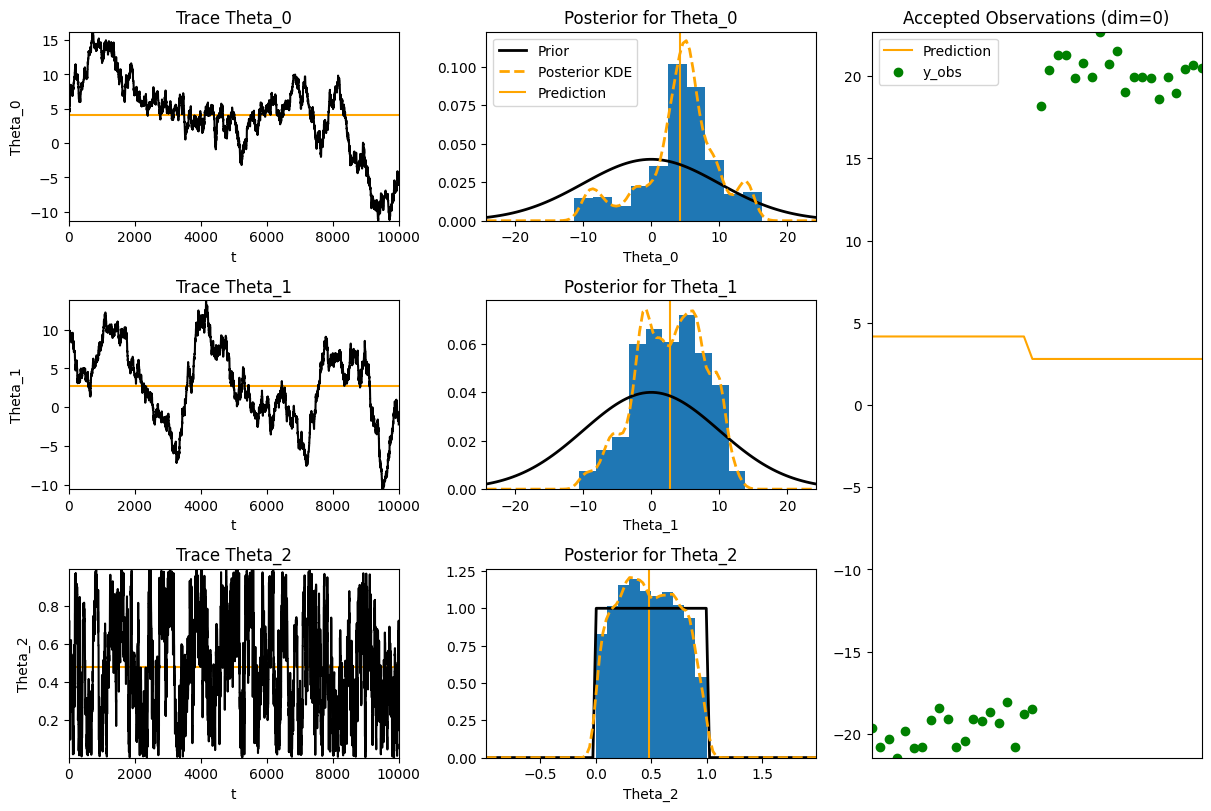
\includegraphics[width=.7\textwidth]{label_switching_MCMC.png}
  %   \caption{Example of ``Label Switching Problem'' when ABC-MCMC is used to fit a Gaussian Mixtures Model with means $\mu_0=20,\mu_1=-20$ and each gaussian has weight $w=0.5$.
  %   \par Theta\_0=$\mu_0$, Theta\_1=$\mu_1$ and Theta_2=$w$.}
  %   \label{fig_label_switching_mcmc}
  % \end{figure}

  \par Due to their more informed search procedure, ABC-MCMC significantly outperforms ABC-Rejection and Importance Sampling in cases where the prior and posterior are very different. This makes ABC-MCMC a better choice in cases were informative priors are not known. However, the ABC-MCMC approach perform very poorly with mixtures models, which are becoming increasingly popular, due to the ``Label Switching Problem'' \cite[]{mcmc_methods_and_the_label_switching_problem_in_bayesian_mixture_modeling} which occurs when two, or more, parameters are nonidentifiable when assigned the same priors\footnote{In a gaussian mixtures model with two mixtures. The parameters associated with each mean can be swapped without affecting the fit of the model. This means that under identical priors it is impossible to separate these two parameters.} and thus the posteriors produced for them will be a combination of all of their true posteriors. \cite[]{mcmc_methods_and_the_label_switching_problem_in_bayesian_mixture_modeling} explore the ``Label Switching Problem''.

\subsubsection{ABC-SMC}\label{sec_abc_smc}

  \par Sequential Monte Carlo (SMC) methods\footnote{Originally coined Particle Filters in \cite[]{non_linear_filtering_interacting_particle_resolution}.} approximate a probability distribution by collecting an initial sample which creates a rough approximation of the distribution; and then iteratively refining this approximation by resampling under ever tighter acceptance criteria (Referred to as improving the ``Resolution'' of the approximation). The acceptance criteria are tightened by defining a set of bandwidths $\{\varepsilon_0,\dots,\varepsilon_T\}$ such that $\varepsilon_0\geq\dots\geq\varepsilon_T$ and iterating through this set to determine the bandwidth used in each resampling step. A extension of this approach is to incorporate importance sampling such that the resampling step also involves reweighting accepted samples. This extension is known as Population Monte Carlo (PMC).

  \par The main advantage of SMC methods is that they iteratively make their acceptance criteria stricter. This is ideal for problems where it is hard to predict a good set of acceptance criteria beforehand. There is still an issue of having to define a set of bandwidths $\{\varepsilon_0,\dots,\varepsilon_T\}$ to be used, however I discuss how this can be mitigated for ABC-SMC towards the end of this subsection.

  \par SMC methods are susceptible to ``Loss of Opportunity''. This phenomenon occurs when part of the parameter space is not included in one of the sample sets, as this means that part of the parameter space can never be sampled from in the future. This mainly occurs to regions of the parameter space where little probability mass is placed, but can occur to denser areas if the sample size is too small. This issue can never be eliminated, except for very simple distributions, do the practical limits on the sample size but can be mitigated by increasing the sample size.

  \par \cite[]{SMC_wo_likelihood} presents the first SMC approach to ABC, but this approaches produces a biased approximation of the posterior, mainly due to it underestimating the tails of the distributions caused by how they originally proposed to evaluate the likelihood ratio. \cite[]{adaptive_ABC} presents an SMC approach to ABC which incorporates importance sampling and an optimised adaptive strategy. This is the version of ABC-SMC I discuss in this section.

  \begin{box_algorithm}[ABC-SMC]\label{alg_abc_smc}
    Adapted from \cite[]{adaptive_ABC}.
    \par
    \begin{algorithm}[H]
      \everymath={\displaystyle}
      \SetKwIF{With}{}{Else}{with probability}{}{}{otherwise}{}
      \SetKwInOut{Require}{require}
      \Require{Observed values $x_{obs}$; Summary statistics $s(\cdot)$; Theorised model $f(X|\cdot)$; Prior Distributions $\pi_0(\theta)$ Distance Measure $\|\cdot\|$; Acceptance Kernel $K_\varepsilon(\cdot)$; Set of Bandwidths $\{\varepsilon_0,\dots,\varepsilon_T\}$; Number of Iterations $T$; Sample Size $N$.}
      $s_{obs}\leftarrow s(x_{obs})$.\\
      \BlankLine
      \# Initial Sample Step\\
      $\tilde\Theta_0\leftarrow\{\}$.\label{alg_abc_smc_initial_sample_start}\\
      $i\leftarrow0$\\
      \While{$i<N$}{
        $\tilde\theta_0^{(i)}\leftarrow$ sample $\pi_0(\theta)$.\\
        $\tilde{x}_0^{(i)}\leftarrow f(X|\tilde\theta_t^{(i)})$.\\
        $\tilde{s}_0^{(i)}\leftarrow s\left(\tilde{x}_t^{(i)}\right)$.\\
        \With{$K_{\varepsilon_0}\left(\left\|\tilde{s}_{0}^{(i)}-s_{obs}\right\|\right)$} {
          $w_0^{(i)}\leftarrow\frac1N$.\\
          Add $\tilde\theta_0^{(i)}$ to $\tilde\Theta_0$ with weight $\tilde{w}_0^{(i)} $.\\
          $i\leftarrow i+1$
        } \lElse {Pass}\label{alg_abc_smc_initial_sample_end}
      }
      \BlankLine
      \# Resampling Step\\
      \For{$T=1,\dots,T$}{\label{alg_abc_smc_resampling_start}
        $\sigma_{t-1}^2\leftarrow$Sample variance of each parameter dimension in $\tilde\Theta_{t-1}$.\\
        $K^*\leftarrow\text{Normal}(\theta,2\cdot\sigma_{t-1}^2)$.\\
        $\tilde\Theta_t\leftarrow\{\}$.\\
        $i\leftarrow0$\\
        \While{$i<N$}{
          $\tilde\theta_t^{(i)}\leftarrow$ sample $\tilde\Theta_{t-1}$.\\
          $\theta^*\leftarrow K_t^*\left(\tilde\theta_t^{(i)}\right)$.\\
          $\tilde{x}_t^{(i)}\leftarrow f(X|\theta^*)$.\\
          $\tilde{s}_t^{(i)}\leftarrow s\left(\tilde{x}_t^{(i)}\right)$.\\
          \With{$K_{\varepsilon_t}\left(\left\|\tilde{s}_{t}^{(i)}-s_{obs}\right\|\right)$} {
            $\tilde\theta_t^{(i)}\leftarrow\theta^*$.\\
            $\tilde{w}_t^{(i)}\leftarrow\frac{\pi_0\left(\tilde\theta_t^{(i)}\right)}{\sum_{j=1}^Nw_{t-1}^{(j)}\prob\left(K_t^*\left(\tilde\theta_{t-1}^{(j)}\right)=\tilde\theta_{t}^{(i)}\right)}$.\label{alg_abc_smc_importance_weight}\\
            Add $\tilde\theta_t^{(i)}$ to $\tilde\Theta_t$ with weight $\tilde{w}_t^{(i)}$.\\
            $i\leftarrow i+1$.
          } \lElse {Pass}
        }
        \BlankLine
        \# Normalise Weights\\
        \For{$i=1,\dots,N$}{
          $w_t^{(i)}\leftarrow\frac{\tilde{w}_t^{(i)}}{\sum_{i=1}^N\tilde{w}_t^{(i)}}$.\\
          Update weight of $\tilde\theta_t^{(i)}$ in $\tilde\Theta_t$ to be $w_t^{(i)}$.
        }
      }\label{alg_abc_smc_resampling_end}
      \Return{$\tilde\Theta_T:=\left\{\left(\tilde\theta_T^{(1)},w_T^{(1)}\right),\dots,\left(\tilde\theta_T^{(N)},w_T^{(N)}\right)\right\}$}
    \end{algorithm}
  \end{box_algorithm}

  \par \textbf{Algorithm \ref{alg_abc_smc}} is the algorithm presented in \cite[]{adaptive_ABC}. This algorithm has two phases: First, (Lines \ref{alg_abc_smc_initial_sample_start}-\ref{alg_abc_smc_initial_sample_end}) generating an initial sample of parameters $\tilde\Theta_0$ of size $N$ using standard ABC-Rejection Sampling methods. Each sample is assigned the same importance weight $1/N$; Second, the \textit{Resampling Step} (Lines \ref{alg_abc_smc_resampling_start}-\ref{alg_abc_smc_resampling_end}). This involves resampling from the previously set of accepted parameter samples $\tilde\Theta_{t-1}$ with the probability of sampling each parameter equal to its importance weight. Each sample $\tilde\theta$ is perturbed using a perturbation kernel $K^*(\cdot)$ to generate a new set of parameters $\theta^*$. The new parameter set $\theta^*$ is used to simulate a set of summary statistic values $\tilde{s}$ and a rejection sampling step is used to accepted the new parameter set with probability $K_{\varepsilon_t}\left(\left\|\tilde{s}-s_{obs}\right\|\right)$. Note that the acceptance criteria are tightened each iteration. Each accepted parameter set is assigned an importance weight $\tilde{w}$. The importance weights are normalised after each resampling phase so that they sum to one and thus represent a probability distribution, which is important for sampling from this set.

  \par The importance weight $\tilde{w}$ assigned in Line \ref{alg_abc_smc_importance_weight} is the prior probability for the accepted parameter set divided by the probability of that parameter set under the posterior $\hat\pi_t$ generated by the previous step. This is just the standard importance weighting of the likelihood ratio. Note that each resampling step is aiming to produce a more refined version of the posterior distribution generated by the previous step, and thus the previous distribution is the target distribution and the prior is the originally proposed distribution.

  \[ \tilde{w}_t^{(i)}:=\frac{\pi_0\left(\tilde\theta_t^{(i)}\right)}{\hat\pi_t\left(\theta_t^{(i)}\right)}\text{ where }\hat\pi_t\left(\theta_t^{(i)}\right)=\sum_{j=1}^Nw_{t-1}^{(j)}\prob\left(K_t^*\left(\tilde\theta_{t-1}^{(j)}\right)=\tilde\theta_{t}^{(i)}\right) \]

  \par The adaptive feature of \textbf{Algorithm \ref{alg_abc_smc}} is the setting of the perturbance kernel $K^*$. The perturbance kernel used in \textbf{Algorithm \ref{alg_abc_smc}} is a component-wise random walk kernel which perturbs each component of the parameter set independently by adding additive gaussian noise to them. The variance of this gaussian noise is equal to twice the sample variance of the accepted samples from the previous phase.

  \[ \left[\sigma_{t-1}^2\right]_i=\frac1{N-1}\sum_{j=1}^N\left(\left[\tilde\theta_{t-1}^{(j)}\right]_i-\left[\bar\theta_{t-1}\right]_i\right)^2 \]
  where $\bar\theta_{t-1}$ is the sample mean of the previous set of accepted samples.

  \par Using a component-wise random walk kernel is ideal for an adaptive algorithm as it is straightforward to implement and is computationally efficient as simple closed-form expressions for the probabilities required to calculate the importance weight for each accepted parameter set.

  \par The variance is set to twice the sample variance of the previously accepted set as this minimises the Kullback-Leibler divergence between the target distribution (two independent parameter samples) and proposed distribution ( generating a set of parameters by perturbing another) for the component-wise random walk kernel being used. % TODO proof https://arxiv.org/pdf/0805.2256.pdf pg 5
  Minimising Kullback-Leibler divergence means the two distributions are increasingly similar. See \cite[]{on_optimality_of_kernels_for_approximate_bayesian_computation_using_SMC} for discussion of other optimal perturbation kernels for ABC-SMC.

  \par The calculation of the importance weight for each accepted parameter, during resampling, requires summing over all the parameter sets from the previously accepted sample set. This means the resample stage takes $O(N^2)$ time and thus the overall run time of the algorithm is $O(TN^2)$ where $T$ is the number of resampling iterations and $N$ is the sample size. In practice the runtime of the algorithm will be dominated by assessing and generating samples, as the majority will be rejected, rather than by calculating the weight for each accepted set.

  \par Each resampling step is dependent on the previous step as it requires the previous set of accepted samples $\tilde\Theta_{t-1}$ in order to generate samples. This means that this part of the algorithm cannot be parallelised. However, the simulations within each resampling step can be parallelised. As well as the initial sample generation step, as discussed in \textit{Section \ref{sec_abc_rejection_sampling}}.

  \par This approach requires the specification of a set of bandwidths $\{\varepsilon_0,\dots,\varepsilon_T\}$. This can be difficult to do in an informed way, and would rather be avoided. Firstly, it is important to note that it is not strictly necessary for the algorithm to use the whole set and rather the algorithm can be stopped after it has reached a certain level of convergence (or number of simulations). Further, there is no need to define a full set of bandwidths at the start of the algorithm, instead an initial bandwidth $\varepsilon_0$ can be defined and then future bandwidths are set adaptively such that a target percentage $\Delta\%$ of previously sample would be accepted. Implementing this is straightforward for most common acceptance kernels, if a uniform acceptance kernel is being used it simply requires setting the next bandwidth to be the $\Delta$ percentile distance among the previously accepted parameter sets.

  \par The need to set the initial bandwidth can be removed too by simply accepting all simulations into the initial sample set $\tilde\Theta_0$, however this would make the algorithm significantly more inefficient as the initial sample with simple resemble the prior. Further, unless the sample size is very large there will be a high level of ``Loss of Opportunity''. A better approach would be to use the ``Best Samples'' variation of ABC-Rejection Sampling (\textbf{Algorithm \ref{alg_abc_rejection_best}}).

  \par Incorporating this adaptive approach to bandwidth selection removes the need to define a set of bandwidths $\{\varepsilon_0,\dots,\varepsilon_T\}$ or the number of iterations $T$; and replaces them with defining an acceptance rate and number of simulations for the ``Initial Sample Step'', a target acceptance rate between resampling iterations and a maximum number of simulations. These are significantly easier hyperparameters to define as their affects are much more apparent and predictable.

  % TODO perturbation kernels https://arxiv.org/pdf/1106.6280.pdf

\subsection{ABC for Model Choice}\label{sec_abc_model_choice}

  \begin{box_definition}[Bayes Factor, \cite{bayes_factors}]
    Consider two models $M_1,M_2$ and some observed data $x_{obs}$. The Bayes Factor $B_{1,2}$ for data $x_{obs}$ coming from model $M_1$ rather than model $M_2$ is the ratio of the likelihood ratio of $x_{obs}$ coming from $M_1$ rather than $M_2$.
    \[ B_{1,2}:=\frac{\prob(x_{obs}|M_1)}{\prob(x_{obs}|M_2)} \]
    \cite[]{theory_of_probability} gives a qualitative assessment of Bayes Factor: ``1 to 3 is barely worth a mention, 3 to 10 is substantial, 10 to 30 is strong, 30 to 100 is very strong and over a 100 is decisive evidence in favour of model $M_1$. Values below 1 take the inverted interpretation in favour of model $M_2$.''
    \par
  \end{box_definition}

  Bayes Factor is a metric used to determine which of two models is more likely to have generated some observed data. Bayes Factor can be restated in terms of posteriors, using Bayes rule, as follows.
  \[ B_{1,2}(x_{obs}):=\frac{\prob(x_{obs}|M_1)}{\prob(x_{obs}|M_2)}=\frac{\frac{\prob(x_{obs})\prob(M_1|x_{obs})}{\prob(M_1)}}{\frac{\prob(x_{obs})\prob(M_2|x_{obs})}{\prob(M_2)}}=\frac{\prob(M_2)\prob(M_1|x_{obs})}{\prob(M_1)\prob(M_2|x_{obs})} \]
  where $\prob(M_i)$ is the prior weight given to model $M_i$. It is generally reasonable to assume equal prior likelihood for each model. Under this assumption Bayes factor is the same as the posterior ratio which is readily estimatable from ABC methods as the ratio of probabilities that the models generate $x_{obs}$.

  \[ B_{1,2}(x_{obs})=\frac{\prob(M_1|x_{obs})}{\prob(M_2|x_{obs})} \]

  \begin{box_algorithm}[ABC Model Choice ``Rejection Sampling'']\label{alg_abc_mc}
    Adapted from \cite[]{abc_likelihood_free_methods_for_model_choice_in_gibbs_random_fields}.
    \begin{algorithm}[H]
      \SetKwIF{With}{}{Else}{with probability}{}{}{otherwise}{}
      \SetKwInOut{Require}{require}
      \Require{Observed values $x_{obs}$; Summary statistics $s(\cdot)$; Priors for Models $\pi_M(M)$; Theorised models $M_1(X|\theta_{M_1}),M_2(X|\theta_{M_2})$; Parameter Priors for each model $\pi_{M_1}(\theta_{M_1}),\pi_{M_2}(\theta_{M_2})$; Acceptance Bandwidth $\varepsilon$; Distance Measure $\|\cdot\|$; Target Number $M$.}
      $s_{obs}\leftarrow s(x_{obs})$.\\
      $\mathcal{M}\leftarrow\{\}$.\\
      $t\leftarrow1$.\\
      \While{$t\leq M$}{
        $m_t\leftarrow$ sample $\pi_M(M)$.\\
        $\tilde\theta_t\leftarrow$ sample $\pi_{m_t}(\theta)$.\\
        $\tilde{x}\leftarrow f(X|\tilde\theta_t)$.\\
        $\tilde{s}\leftarrow s\left(\tilde{x}\right)$.\\
        \If{$\|s_{obs}-\tilde{s}\|\leq\varepsilon$} {
          $\hat\theta^{(t)}\leftarrow\tilde\theta$.\\
          Add $m_t$ to $\mathcal{M}$.\\
          $t\leftarrow t+1$
        } \lElse {Pass}
      }
      \Return{$\mathcal{M}=\{m_1,\dots,m_M\}$}
    \end{algorithm}
  \end{box_algorithm}

  \par \cite[]{abc_likelihood_free_methods_for_model_choice_in_gibbs_random_fields} present an algorithm which uses an alteration of the ABC-Rejection Sampling algorithm, using a uniform kernel, to estimate Bayes Factor. Their approach is outlined in \textbf{Algorithm \ref{alg_abc_mc}}. This approach defines a meta-model $M=(M_1,M_2)$ which is a mixtures model which uses model $M_1$ or $M_2$ according to some distribution $\pi_M$. The distribution $\pi_M$ indicates our prior belief of the likelihood of each model. The algorithm then proceeds as a standard ABC-Rejection sampling algorithm except during the parameter sampling step it also samples which model to use (this defines which set of parameter priors to use too). Each time a simulation is accepted, the model which generated it is recorded in the set $\mathcal{M}$. The returned set $\mathcal{M}$ provides the ratio of the number of times simulations from each model were accepted which estimates Bayes Factor.

  \[ \hat{B}_{1,2}=\frac{\sum_{i=1}^N\mathbbm{1}\{m_i=M_1\}}{\sum_{i=1}^N\mathbbm{1}\{m_i=M_2\}} \]
  % TODO better justification

  \par The results of \textbf{Algorithm \ref{alg_abc_mc}} are sensitive to how informative the priors are for each model and thus can be used to compare different prior sets.


  \par This approach is based on the ABC-Rejection Sampling algorithm and thus does not gain any of the advantages of the ABC-MCMC or ABC-SMC algorithms, namely being effective when the prior and posterior are significantly different. \cite[]{abc_scgene_for_parameter_inference_and_model_selection_in_dynamical_systems} present a model selection algorithm which uses ABC-SMC but requires the use of a meta-model which incorporates the models being tested, as in \cite[]{abc_likelihood_free_methods_for_model_choice_in_gibbs_random_fields}. \cite[]{likelihood_free_estimation_of_model_evidence} present an approach which estimates the evidence for each model independently, using ABC-SMC.

\subsection{Regression Adjustment in ABC}\label{sec_abc_regression_adjustment}

  \par Regression adjustment in ABC is an innovation first suggest by \cite[]{ABC_in_population_genetics} where the regression methods are applied to the accepted parameter sets in order to reduce the distance between the observed summary statistic value $s_{obs}$ and the simulated summary statistic values $\tilde{s}$. Reducing this distance results in an improved approximation. This step is applied after a set of accepted simulations $\tilde\Theta$ has been produced.

  \par The approach suggested in \cite[]{ABC_in_population_genetics} performs weighted local-linear regression of the accepted parameter values $\theta$ on the difference between their summary statistic values and those of the observed model $(s-s_{obs})$. Standard linear regression assumes the following relationship exists

  \[ \theta=\alpha+s^T\beta+\varepsilon\quad\alpha\in\mathbb{R}^{\rho},\beta\in\mathbb{R}^{\rho\times\rho},\varepsilon\in\mathbb{R}^\rho \]

  where $\rho:=|\theta|$ is the number of parameters and $\varepsilon$ is independent additive gaussian noise with zero mean and constant variance. However, it is generally unrealistic that such a relationship or properties of $\varepsilon$ hold for the whole sufficient-statistic space, but these may hold in the locality of $s_{obs}$. This is why Beaumont \textit{et al.} suggest local-linear regression, which assumes the following relationship.

  \[ \theta=\alpha+(s-s_{obs})^T\beta+\varepsilon \]

  \par When taking a least-squares approach to this regression problem, the objective function is to find the following:

  \begin{equation}\label{eqn_regression_objective}
    \hat\alpha,\hat\beta=\text{argmin}_{\alpha,\beta}\sum_{i=1}^N\left(\tilde\theta_i-\left\{\alpha-(\tilde{s}_i-s_{obs})^T\beta\right\}\right)^2K_\varepsilon\left(\|\tilde{s}_i-s_{obs}\|\right)
  \end{equation}

  where $N$ is the number of accepted parameter sets, $\tilde\theta_i$ is the $i^{th}$ accepted parameter set, $\tilde{s}_i$ is the summary statistic values associated with $\tilde\theta_i$, $\|\cdot\|$ is a distance function and $K_\varepsilon(\cdot)$ is a kernel density function with bandwidth $\varepsilon$. Beaumont \textit{et al.} recommend using the Epanechnikov kernel as doing so means that few simulations will be assigned small, but non-zero, weights. Having lots of such weightings is computationally inefficient as they still need to be assessed but offer little insight.

  \par The solution to (\ref{eqn_regression_objective}) is the following

  \[\everymath={\displaystyle}\begin{array}{rrl}
    \left(\hat\alpha_{LSE},\hat\beta_{LSE}\right)&:=&(X^TWX)^{-1}X^TW\pmb\theta\\
    \text{where}\\
    X&:=&\begin{pmatrix}
      1&(\tilde{s}_{1,1}-s_{obs,1})&\dots&(\tilde{s}_{1,M}-s_{obs,M})\\
      1&(\tilde{s}_{2,1}-s_{obs,1})&\dots&(\tilde{s}_{2,M}-s_{obs,M})\\
      \vdots&\vdots&\ddots&\vdots\\
      1&(\tilde{s}_{N,1}-s_{obs,1})&\dots&(\tilde{s}_{N,M}-s_{obs,M})
    \end{pmatrix}\\
    W&:=&\begin{pmatrix}
      K_{\varepsilon}(\|\tilde{s}_1-s_{obs}\|)&0&\dots&0\\
      0&K_{\varepsilon}(\|\tilde{s}_2-s_{obs}\|)&\dots&0\\
      \vdots&\vdots&\ddots&\vdots\\
      0&0&\dots&K_{\varepsilon}(\|\tilde{s}_N-s_{obs}\|)
    \end{pmatrix}\\
    \pmb\theta&:=&(\tilde\theta_1,\dots,\tilde\theta_N)^T
  \end{array}\]
  $\hat\alpha_{LSE}$ is the first column of the resulting matrix and $\hat\beta_{LSE}$ is the remaining columns.

  \par These solutions imply the following general relationship between summary statistic values $s$ and the expected parameter set to have generated them, for values of $s$ in the region of $s_{obs}$.

  \[ \hat\expect[\theta|s]=\hat\alpha_{LSE}+\hat\beta_{LSE} \]

  \par This relationship is used to define a mean-corrected parameter set $\theta_i^*$ each accepted parameter set $\theta_i$ by removing the expected difference between the parameters which produce $s_i$ and $s_{obs}$.

  \[\begin{array}{rcl}
    \theta_i^*&:=&\theta_i-\left(\hat\expect[\theta|s_i]-\hat\expect[\theta|s_{obs}]\right)\\
    &=&\theta_i-(\hat\alpha_{LSE}+s_i^T\hat\alpha_{LSE})+(\hat\alpha_{LSE}+s_{obs}^T\hat\alpha_{LSE})\\
    &=&\theta_i+(s_{obs}-s_i)^T\hat\beta_{LSE}
  \end{array}\]

  Note that it is possible for the corrected parameter sets $\theta^*$ to fall outside of the priors. There are ways to address this, but this should be taken as a sign that different priors should be used as it means the regression is extrapolating rather than interpolating.

  \par In \cite[]{ABC_in_population_genetics} simulation experiments on the Growing Population Model of \cite[]{population_growth_of_human_Y_chromosomes} are run to compare methods which implement their regression adjustment, to those that don't. They found that using regression adjustment meant that ABC-Rejection Sampling had less of a tendency to stay close to the prior. And, that acceptance kernel bandwidth had less of an effect when regression adjustment was applied. This suggests that using regression adjustment increases the rate of convergence.

  \par Implementing this regression method is fairly straightforward as it is applied after all other steps in standard ABC-methods and there are many programming packages available which can perform local-linear weighted regression efficiently. There is an increased  space requirement for algorithms which use this approach as they now need to store the summary statistic values for each accepted parameter set. This should approximately double the space used as it is generally efficient to use one summary statistic per parameter (See \textit{Section \ref{sec_summary_stats}}). This is not a major concern as space requirements are rarely a limiting factor for ABC methods, but it is worth being aware of.

  \par \cite[]{statistical_evaluation_of_alternative_models_of_human_evolution} required 10 CPU months to estimate the parameters of their complex model using the regression method of \cite[]{ABC_in_population_genetics}. This is unsurprising as this approach requires the inversion of a matrix whose size is dependent on the number of summary statistics being used and the number of parameter sets which has been accepted.

  % TODO second regression step (see notebook)

  \begin{center}
    \noindent\rule{.8\textwidth}{0.4pt}
  \end{center}

  \par \cite[]{non_linear_regression_models_for_abc} present using a shallow neural network for nonlinear heteroscedastic regression of parameter values on the summary statistic values, they compare an adaptive and a non-adaptive approach. Their aim was to reduce the computational load required to perform this regression, compared to the approach in \cite[]{ABC_in_population_genetics}. In their worked examples their approaches require significantly less computational time.

  \par In their the bandwidth had little affect on their neural network approaches, compared to the approach of \cite[]{ABC_in_population_genetics}. And, that the posterior quantiles were typically tighter for their neural network methods too and were more centred around the true parameter value. This suggests the neural network methods produce a more accurate fit.

  \par The limitations to the approach of \cite[]{non_linear_regression_models_for_abc} are the same as with most uses of neural networks: overfitting and lack of interpretability. I discuss these issues in more detail in \textit{Section \ref{sec_non_linear_projection}}.

\newpage
\section{Summary Statistic Selection}\label{sec_summary_stats}

  % TODO posterior mean are optimal summary statistics

  In this section I motivate the research into summary statistic selection \textit{Section \ref{sec_summary_stats_motivation}} and discuss features to consider when selecting summary statistics \textit{Section \ref{sec_properties_of_summary_statistics}}. I then describe five methods for summary statistic selection methods: three which use hand-crafted summary statistics \textit{Sections \ref{sec_approximate_sufficient_subset}-\ref{sec_two_step_minimum_entropy}}; and two which automatically generate summary statistics \textit{Sections \ref{sec_semi_automatic_abc}-\ref{sec_non_linear_projection}}. These approaches are covered in the chronological order in which they were original proposed. To close the section I use a toy example of an SIR model to compare these methods \textit{Section \ref{sec_summary_statistics_toy}}.

% TODO Fisher information matrix.

\subsection{Motivation}\label{sec_summary_stats_motivation}

  % TODO - there would be little reason to use summary statistics if it wasn't for computational limitations (otherwise use whole dataset)

  % TODO curse of dimensionality applies to having too many summary statistics

  \par The study of summary statistics has relevance beyond ABC methods, largely due to the recent ``Big-Data Revolution'' which has seen the rate at which data can be collected and stored significantly outpace improvements in computational power. This has motivated research into effective methods to reduce the size of datasets so that more computationally intensive algorithms can be used to analyse the data. % TODO give examples of papers from other fields

  \par A summary statistic $s$ is a statistic which reduces the dimensionality of some sampled data, in a deterministic fashion, whilst retaining as much information about the sampled data as possible. Reducing the dimensionality of data is desirable as it reduces the computational requirements to analyse the data. Ideally, a summary statistic would compress the sampled data without any information loss (A property known as ``sufficiency''). However, low-dimension sufficient summary statistics are rare in practice and we often have to trade-off information retention against dimensionality reduction.

  \[ s:\mathbb{R}^m\to\mathbb{R}^p\text{ with }m>p \]

  \par In most cases each dimension of the output of a summary statistic is the result of an independent calculation. As such, it is often conceptually easier to consider each dimension as an independent summary statistics when selecting summary statistics. This idea of each dimension of independence also makes it conceptually easy to combine summary statistics by appending the result of one statistic onto the end of the other, as new dimensions. % TODO reword or expand this (probs move)
  As long as the sum of the dimensions of the outputs from the summary statistics in the set is less than that of the sampled data, then using a set of summary statistics still produces effective dimensionality reduction.

  \[ m>\sum_{i=1}^kp_i\text{ where }s_i:\mathbb{R}^m\to\mathbb{R}^{p_i} \]

  The success of ABC methods depends mainly on three user choices: choice of summary statistic; choice of distance measure; and choice of acceptance kernel. Of these, summary statistic choice is arguably the most important as the other two mainly affect the rate at which the algorithm converges on the posterior mean. Whereas, choosing summary statistics which are uninformative can lead to the parameter posteriors returned by the algorithm being drastically different from the true parameter posteriors. This is trivial to realise if you consider a scenario where $s(x)=c$, for some constant $c\in\mathbb{R}$, is used as the sole summary statistic as this would result in all (or none) of the simulations being accepted as thus the returned posterior will be the same as the supplied prior.

  \par In practice, the quality of the posteriors returned from an ABC method is limited by the amount of computational time which is dedicated to running the algorithm. For some problems, such as ......... % TODO
  , it is reasonable to dedicate the majority of your computing time on summary statistic selection, rather than on model fitting, as it is clear that even the simplest ABC methods (e.g. ABC-Rejection Sampling) will be sufficient to fit the model, given a good choice of summary statistics.

  \subsection*{Traditional Thinking}\label{sec_summary_stats_traditional_thinking}

  \par Traditionally, summary statistics for ABC methods are chosen manually using expert, domain-specific knowledge. Utilising this expert knowledge is desirable as these statistics will incentivise exploring regions of the parameter space which have been scientifically shown to be relevant to the given problem and thus more likely to contain the true parameter values (Similarly, these statistics will disincentivise exploring regions which have been shown to not be of interest). % TODO re-write this sentence

  % TODO - Having a more mathematically rigourous approach is desirable

  \par However, relying on expert knowledge to choose summary statistics limits the scenarios where ABC methods can be applied to only those where there has already been significant research. And, leads to statistics being chosen due to their prevalence in a field rather than their suitability to computational methods. Moreover, the use of hand-crafted summary statistics means that any limitations in current understanding of a field will be encoded into the model fitting process, possibly leading to misspecification.

  \par When using a set of summary statistics, expert knowledge is generally not sufficient to determine how best to weight each summary statistic. Some of the methods I describe below can be used to automate the process of determining these weights by specifying multiple versions of the same summary statistic, with each version having a different weight. % TODO mention that this is not easy to implement due to easy pitfalls

\subsection{Properties of Summary Statistics}\label{sec_properties_of_summary_statistics}

  % Degree reduction (ie greater compression)
  \par When evaluating a summary statistic for use in ABC there are main properties, both practical and mathematical, to consider.

  \par A useful mathematical property, observed in \cite[]{statistical_inference_for_noisy_nonlinear_ecological_dynamic_systems}, that asymptotically summary statistics typically have a normal distribution $s\sim\text{Normal}(\mu_s,\Sigma_s)$ with mean $\mu_s$ and covariance matrix $\Sigma_s$. This property can be used to motivate a regression adjustment approach, as explored in \textit{Section \ref{sec_abc_regression_adjustment}}, using the sample estimates of mean and co-variance.

\subsection*{Practical Properties}

  \par The key reason for using summary statistics is for the computational efficiencies which result from their dimensionality reduction. Reducing the size of a dataset means less operations need to be performed to analyse it, meaning more simulations can be processed in the same time-period. This naturally means summary statistics which result in greater dimensionality reduction are preferable, but similarly means that a summary statistic which is computationally inefficient to calculate is less desirable.

  % Computational efficiency & overflow
  % TODO correlation is very inefficient as it considers many
  \par For a model which produces data of dimension $n\times m$ (i.e. $n$ readings, each with $m$ features) most standard summary statistics are calculated in $O(n\cdot m)$  time. However, this is only a theoretical result and in practice there are meaningful differences in the computational requirements of each summary statistics. Calculating the mean and maximum values for each feature takes $O(n\cdot m)$ time in theory but, since calculating the mean relies on arithmetic operations and the maximum on comparison operations, they will take different amounts of time in practice. Statistics which rely on search or sorting operations (most notably order statistics) are variable in the their time complexity for different data sets which will affect the reliability of models which use them. Integer overflow is a possible issue for some summary statistics, although this is often easy to avoid when actively being considered during the implementation of an algorithm. Moreover, for statistics with non-linear computational complexity (e.g. correlation between each pair of features), the size of the dataset being analysed needs to be considered when evaluating summary statistic choice.

  % weights and scaling
  \par ABC-methods rely on distance measures to determine whether a simulation is good, or not. This means that the range and scale of values a summary statistic will likely produce will have an affect on how influential that summary statistic is to the final model fit. In most cases it is reasonable to standardise all statistics to have the same mean and variance, effectively giving the same weighting to each statistic. This can be implemented to occur adaptively within the ABC-method. There may be cases % TODO are there any?
  where assigning different weights to different summary statistics makes sense, and produces a better model fit, but these are hard to justify from a theoretical approach. The selection methods I discuss which compare hand-crafted statistics (Sections \ref{sec_approximate_sufficient_subset}-\ref{sec_two_step_minimum_entropy}) can be used to compare possible weightings by including several versions of the same summary statistic, each with a different scaling, in the set of statistics being compared. This will however increase computation time due to the increase size of the set of statistics and may make the results harder to interpret\footnote{Multiple sets of weighted summary statistics will be equivalent due to having the same ratio of weights}.

  % Interpretability
  \par For real-world modelling problems, the interpretability of summary statistics used in the final model is a key factor in how useful the solution is. Senior stakeholders in a problem will want to use the final model to justify their future decisions, this is much easier to do when the factors the model is considering, and the weights it assigns to them, are readily understandable. Hand-crafted statistics are almost always the most readily understandable statistics, as such generated statistics are rarely used in commercial problems\footnote{The current popularity of using ``Neural Networks'' in commercial settings does buck this trend. I hope this fad will subside soon in favour of more interpretable alternatives. I believe it is worth noting that the new European Union payment services directive (PSD2) requires that certain models used by financial institutions be ``explainable'' in order to improve the customer experience and to ensure no one is discriminated against due to their protected characteristics.}. In cases where it is chosen to use automatically generated statistics; one can develop an intuition for their model by varying the inputs, or removing certain features, and observing how the output varies. This is naturally harder to

\subsection*{Sufficiency}\label{sec_sufficiency}
  % \subsubsection*{Theory}

  \begin{box_definition}[Sufficient Statistic \cite{sufficient_statistics}]\label{def_sufficient_statistic}
    Let $s:\mathbb{R}^m\to\mathbb{R}^n$ be a statistic and $X$ be a model with parameters $\theta$. The statistic $s$ is said to be sufficient for the parameters $\theta$ if the conditional distribution of the model $X$, given the value of the statistic $s(X)$, is independent of the model parameter.
    \[ \prob(X|s(X))=\prob(X|s(X),\theta) \]
  \end{box_definition}

  \par Verbosely, a statistic is sufficient for a model parameter(s) if it captures all the information which a sample of the model carries about said parameter(s). This means that knowing the value of a sufficient statistic is as informative as knowing the true model parameters. This is clearly a desirable property as in practice we can always calculate the value of the summary statistic using the sampled data, but cannot know the true parameter values (otherwise we would not be trying to predict them). Sufficient statistics exist for all models as, trivially, the identity function is a sufficient statistic for all models.

  \par It can be intuitively helpful to consider a sufficient statistic as a data reduction method. Moreover, a sufficient summary statistic provides a loss-less compression of sampled data as it reduces the dimensionality of the data but retains all relevant information.

  \begin{box_remark}[Supersets of Sufficient Statistics]\label{the_sufficiency_of_superset}
    Let $s_{1:k-1}(\cdot):=\{s_1(\cdot),\dots,s_{k-1}(\cdot)\}$ be a collection of $k-1$ summary statistics and suppose that $s_{1:k-1}$ is sufficient for the parameters $\theta$ of some model $X$. Then $s_{1:k-1}\cup\{s_k\}$ is also sufficient for the parameters $\theta$, for all summary statistics $s_k$.
    \begin{proof}
      \everymath={\displaystyle}
      Consider a model with parameters $\theta$ and let $s_1,\dots,s_k$ be summary statistics where the set $s_{1:k-1}:=\{s_1,\dots,s_{k-1}\}$ is sufficient for parameter $\theta$. Note that the likelihood of set $s_k:=s_{1:k-1}\cup\{s_k\}$ given the model parameters $\theta$ can be stated as
      \[ \prob(s_{1:k}(X)|\theta)=\prob(s_k(X)|s_{1:k-1}(X),\theta)\prob(s_{1:k-1}|\theta) \]
      Now consider the following decomposition of the posterior for the model parameters $\theta$ given summary statistics $s_{1:k}$
      \[\begin{array}{rcl}
        \prob(\theta|s_{1:k}(X))&=&\frac{\prob(s_{1:k}(X)|\theta)\prob(\theta)}{\prob(s_{1:k}(X))}\\
        &=&\frac{\prob(s_k(X)|s_{1:k-1}(X),\theta)\prob(s_{1:k-1}|\theta)\prob(\theta)}{\prob(s_k(X)|s_{1:k-1}(X))\prob(s_{1:k-1}(X))}\\
      \end{array}\]
      Since the set $s_{1:k-1}$ is sufficient for $\theta$ we have that
      \[ \prob(s_k(X)|s_{1:k-1}(X))=\prob(s_k(X)|s_{1:k-1}(X),\theta)\]
      Applying this result to the decomposition above, we deduce that the posterior for the model parameters $\theta$ given $s_{1:k}$ or $s_{1:k-1}$ are identical.
      \[\begin{array}{rcl}
        \prob(\theta|s_{1:k}(X))&=&\frac{\prob(s_k(X)|s_{1:k-1}(X),\theta)\prob(s_{1:k-1}|\theta)\prob(\theta)}{\prob(s_k(X)|s_{1:k-1}(X),\theta)\prob(s_{1:k-1}(X))}\\
        &=&\frac{\prob(s_{1:k-1}|\theta)\prob(\theta)}{\prob(s_{1:k-1}(X))}\\
        &=&\prob(\theta|s_{1:k-1}(X))
      \end{array}\]
      Thus the set $s_{1:k}$ is sufficient for model parameters $\theta$. Due to the arbitrary nature of $s_{1:k-1}$ and $s_k$, this result holds for all supersets of sufficient summary statistics.
    \end{proof}
  \end{box_remark}

  \par \textbf{Remark \ref{the_sufficiency_of_superset}} states that if we have a set of summary statistics which are sufficient for a set of parameters, then adding more summary statistics will never increase (or decrease) the amount of relevant information being extracted from the sampled data. This means there is an optimally minimal number of summary statistics required to achieve sufficiency.

  \par I demonstrate in \textbf{Example \ref{example_sufficient_stats_normal}} that the sample mean is a sufficient summary statistic for a normal distribution with unknown mean.

  \begin{box_example}[Sufficient Statistic for Normal Distribution with Unknown Mean]\label{example_sufficient_stats_normal}
    \everymath={\displaystyle}
    \par\par Let $X\sim\text{Normal}(\mu,\sigma^2_0)$, with $\mu\in\mathbb{R}$ unknown and $\sigma_0^2\in\mathbb{R}$ known, and $\mathbf{x}$ be $n$ independent observations of $X$.
    \par We have that
    \[
      f_{\mathbf{X}}(\mathbf{X})=\prod_{i=1}^nf_X(X_i)=\frac1{(2\pi\sigma_0^2)^{n/2}}\exp\left\{-\frac1{2\sigma_0^2}\sum_{i=1}^n(X_i-\mu)^2\right\}
    \]
    Let $s=s(\mathbf{X})$ be an arbitrary statistic of $n$ observations from the model. We will build up the conditional distribution of $\mathbf{X}$ given $s(\mathbf{X})$, by first considering their joint distribution
    \[\begin{array}{rcl}
      f_{\mathbf{X},s(\mathbf{X})}(\mathbf{X},s)&=&\frac1{(2\pi\sigma_0^2)^{n/2}}\exp\left\{-\frac1{2\sigma_0^2}\sum_{i=1}^n(X_i+s-s-\mu)^2\right\}\\
      &=&\frac1{(2\pi\sigma_0^2)^{n/2}}\exp\left\{-\frac1{2\sigma_0^2}\sum_{i=1}^n((X_i+s)-(\mu-s))^2\right\}\\
      &=&\frac1{(2\pi\sigma_0^2)^{n/2}}\exp\left\{-\frac1{2\sigma_0^2}\sum_{i=1}^n\left((X_i-s)^2+(\mu-s)^2-2(\mu-s)(X_i-s)\right)\right\}\\
      &=&\frac1{(2\pi\sigma_0^2)^{n/2}}\cdot\exp\left\{-\frac1{2\sigma_0^2}\sum_{i=1}^n(X_i-s)^2\right\}\cdot\exp\left\{-\frac1{2\sigma_0^2}\sum_{i=1}^n(\mu-s)^2\right\}\\
      &&\cdot\exp\left\{-\frac1{2\sigma_0^2}\sum_{i=1}^n-2(\mu-s)(X_i-s)\right\}\\
      &=&\frac1{(2\pi\sigma_0^2)^{n/2}}\cdot\exp\left\{-\frac1{2\sigma_0^2}\sum_{i=1}^n(X_i-s)^2\right\}\cdot\exp\left\{-\frac1{2\sigma_0^2}\sum_{i=1}^n(\mu-s)^2\right\}\\
      &&\cdot\exp\left\{\frac{\mu-s}{\sigma_0^2}\left(\sum_{i=1}^n(X_i)-ns)\right)\right\}
    \end{array}\]
    If we define $s(\mathbf{X})=\frac1n\sum_{i=1}^nX_i$, the sample mean, then the third exponential disappears. Note that $s(\mathbf{X})\sim\text{Normal}\left(\mu,\frac1n\sigma_0^2\right)$.
    \par Now consider the conditional distribution of $\mathbf{X}$ given $s(\mathbf{X})$.
    \[\begin{array}{rcl}
      f_{\mathbf{X}|s(\mathbf{X})}(\mathbf{X}|s)&=&\frac{f_{\mathbf{X},s(\mathbf{X})}(\mathbf{X},s)}{f_{s(\mathbf{X})}(s(\mathbf{X}))}\\
      &=&\frac{\sqrt{\frac1{\left(2\pi\sigma_0^2\right)^n}}\cdot\exp\left\{-\frac1{2\sigma_0^2}\sum_{i=1}^n(X_i-s)^2\right\}\cdot\exp\left\{-\frac{n}{2\sigma_0^2}(\mu-s)^2\right\}}{\sqrt{\frac{n}{2\pi\sigma_0^2}}\cdot\exp\left\{-\frac{n}{2\sigma_0^2}(\mu-s)^2\right\}}\\
      &=&\sqrt{\frac{1}{n(2\pi\sigma_0^2)^{n-1}}}\cdot\exp\left\{-\frac1{2\sigma_0^2}\sum_{i=1}^n(X_i-s)^2\right\}
    \end{array}\]
    This shows that the conditional distribution of $\mathbf{X}$ given $s(\mathbf{X})$ is independent of $\mu$, the unknown parameter, and thus the sample mean is a sufficient statistic for a normal distribution with unknown mean
  \end{box_example}

  \par \textbf{Example \ref{example_sufficient_stats_normal}} shows that finding sufficient summary statistics can be a highly manually and did require us to ``guess'' at the possible formulation of a summary statistic, then verify that it was sufficient. The Fisher-Neyman factorisation criterion (\textbf{Theorem \ref{fisher_neyman_factorisation_criterion}}) \cite[]{fnf_fisher_part,fnf_neyman_part}, first recognised by Fisher in \cite[]{fnf_fisher_part}, specifies a property which all sufficient statistics have. This property is used as the basis of a more formulaic approach to finding sufficient statistics by separating the terms of the conditional probability of a model given the summary statistic value into those which depend on the summary statistic and those which do not.

  \begin{box_theorem}[Fisher-Neyman Factorisation Criterion \cite{sufficient_statistics}]\label{fisher_neyman_factorisation_criterion}
    \par\par Let $X\sim f(\cdot;\theta)$ be a model with parameters $\theta$ and $s(\cdot)$ be a statistic.
    \par $s(\cdot)$ is a sufficient statistic for the model parameters $\theta$ \underline{iff} there exist non-negative functions $g(\cdot;\theta)$ and $h(\theta)$ where $h(\cdot)$ is independent of the model parameters\footnotemark\footnotetext{i.e. $h(\cdot)$ only depends on the sampled data} and
    \[ f(X;\theta)=h(X)g(s(X);\theta) \]
    This formulation shows that the distribution of the model $X$ only depends on the parameter $\theta$ through the information extracted by the statistic $s$. A consequence of the sufficiency of $s$.
    \begin{proof} \cite[]{fnf_theorem_proof}
      \everymath={\displaystyle}
      \begin{itemize}
        \item[$\Longrightarrow$] First, consider the forwards direction of the theorem and suppose $s$ is a sufficient summary statistic. Define functions
        \[ h(x)=\prob(X=x|s(X)=s(x))\quad\text{and}\quad g(s(x);\theta)=\prob(s(X)=s(x);\theta)\]
        Note that $h(\cdot)$ is independent of the model parameter $\theta$ due to the sufficiency of $s$. Then
        \[\begin{array}{rcl}
          f_X(x)&=&\prob(X=x)\\
          &=&\prob(X=x,s(X)=s(x))\\
          &=&\prob(X=x|s(X)=s(x))\prob(s(X)=s(x))\\
          &=&h(X)g(s(X))
        \end{array}\]
        \item[$\Longleftarrow$] Now, consider the reverse direction of the theorem and suppose there exists some functions $h(\cdot),g(\cdot;\theta)$, with $h(\cdot)$ independent of model parameter $\theta$, such that
        \[ f(x;\theta)=h(x)g(s(x);\theta)\text{ for all }x\in\mathcal{X},\ \theta\in\Theta \]
        where $\mathcal{X}$ is the support of $X$ and $\Theta$ the set of possible parameters.
        \par Then, for an arbitrary $c\in\mathbb{R}$
        \[\begin{array}{rcl}
          \prob(X=x|s(X)=c)&=&\frac{\prob(X=x,s(X)=c)}{\prob(s(X)=c)}\\
          &=&\frac{\indexed\{s(x)=c\}f(x;\theta)}{\sum_{y\in\mathcal{X};s(y)=c}f(y;\theta)}\\
          &=&\frac{\indexed\{s(x)=c\}h(x)g(s(x);\theta)}{\sum_{y\in\mathcal{X};s(y)=c}h(y)g(s(y);\theta)}\\
          &=&\frac{h(x)g(c;\theta)}{\sum_{y\in\mathcal{X};s(y)=c}h(y)g(c;\theta)}\\
          &=&\frac{h(x)}{\sum_{y\in\mathcal{X};s(y)=c}h(y)}
        \end{array}\]
        This final expression is independent of the model parameter $\theta$.
      \end{itemize}
      The result holds in both directions.
    \end{proof}
  \end{box_theorem}

  \par \textbf{Example \ref{example_sufficient_stats_poisson}} below demonstrates how the Fisher-Neyman Factorisation Theorem can be used to find a sufficient summary statistic for a Poisson model where the mean $\lambda$ is unknown

  \begin{box_example}[Using Fisher-Neyman Factorisation Theorem to find sufficient statistics for a Poisson distribution with unknown mean]\label{example_sufficient_stats_poisson}
    \everymath={\displaystyle}
    \par\par Let $X\sim\text{Poisson}(\lambda)$, with $\lambda\in\mathbb{R}^{>}$ unknown, $\mathbf{x}$ be $n$ independent observations of $X$ and $\textstyle\bar{x}:=\frac1n\sum_{i=1}^nx_i$ be the sample mean of these $n$ observations.
    \par Consider the joint distribution of these $n$ observations
    \[\begin{array}{rcl}
      f_{\mathbf{X}}(\mathbf{x})&=&\prod_{i=1}^nf_X(x_i)\\
      &=&\prod_{i=1}^n\frac{\theta^{x_i}e^{-\theta}}{x_i!}\\
      &=&\frac{1}{\prod_{i=1}^nx_i!}\cdot\theta^{\sum_{i=1}^nx_i}e^{-n\theta}\\
      &=&\underbrace{\left\{\frac{1}{\prod_{i=1}^nx_i!}\right\}}_{(1)}\cdot\underbrace{\left\{\theta^{\sum_{i=1}^nx_i}e^{-n\theta}\right\}}_{(2)}
    \end{array}\]
    The last step shows how the terms can be collected into: (1), those which are independent of model parameter $\theta$; and, (2), those which are dependent on model parameter $\theta$. We can how derive the conditions of the Fisher-Neyman Factorisation theorem by inspecting the final expression.
    \par It is apparent that we should define the function $h(\mathbf{x})$ as
    \[ h(\mathbf{x})=\frac1{\prod_{i=1}^nx_i!} \]
    In order to define the function $g(s(\mathbf{x});\theta)$ we first need to define the summary statistic $s(\mathbf{x})$. This is straightforward as all the sampled data $\mathbf{x}$ only occurs in a sum in (2), so we define $\textstyle s(\mathbf{x})=\sum_{i=1}^n x_i$. Meaning we can define $g(\mathbf{x};\theta)$ as
    \[ g(\mathbf{x};\theta)=\theta^{s(\mathbf{x})}e^{-n\theta} \]
    With these definitions we fulfil the conditions of the Fisher-Neyman Factorisation theorem, meaning $s(\mathbf{X})=\sum_{i=1}^nX_i$ is a sufficient statistic for the mean for a Poisson distribution.
  \end{box_example}

  \par In most cases sufficient statistics for a parameter are not unique. Moreover, each sufficient statistic does not necessarily produce the same level of compression. Consider a normal distribution with unknown mean, here both the sample sum and identity function are both sufficient statistics, however the sample sum is a much more desirable statistic to use as it provides compression down to a single dimension. This lack of uniqueness motivates the concept of minimal sufficiency.

  \begin{box_definition}[Minimally Sufficient Statistic, \cite{dictionary_of_statistical_terms}]\label{def_minimally_sufficient_statistic}
    Let $s(\cdot)$ be a sufficient statistic for parameter $\theta$ of model $X$. $s(\cdot)$ is minimally sufficient if for any other sufficient statistic $t(\cdot)$ of parameter $\theta$ there exists a function $f$ which maps $t(x)\mapsto s(x)$.
    \[ s(X)=f(t(X)) \]
  \end{box_definition}

  \par Minimally sufficient statistics have lower (effective) dimensionality than their non-minimal counterparts. This makes minimally sufficient statistics desirable as they produce the greatest level of compression and, in doing so, maximally reduce the computational resources required to analyse the sampled data.

  \par As with identifying sufficient statistics, determining whether, or not, a sufficient statistic is minimally sufficient is not a trivial task. I demonstrate this in \textbf{Example \ref{example_minimally_sufficient_bernoulli}}.

  \begin{box_example}[Minimally Sufficient Statistic for IID Bernoulli Random Variables]\label{example_minimally_sufficient_bernoulli}
    Let $X_1,\dots,X_n$ are independent and identically distribution Bernoulli random variables. Note that the identity function $s_1(\mathbf{X})=\mathbf{X}$ and the sum function $s_2(\mathbf{X})=\sum_{i=1}^nX_i$ are both sufficient statistics.
    \par We can map from $s_1$ to $s_2$ as follows
    \[ s_2(\mathbf{X})=\sum_{i=1}^n [s_2(\mathbf{X})]_i \]
    However, there is no function which can map from $s_2$ to $s_1$ as it would have to map the value 1 to both $(1,0,\dots,0)$ and $(0,1,\dots,0)$. This proves that the identity function $s_1$ is not a minimally sufficient statistic, but does not prove that the sum function $s_2$ is a minimally sufficient statistic as we have not considered all possible sufficient statistics for this distribution.
  \end{box_example}

  \begin{box_theorem}[Condition for Minimal Sufficiency, \cite{minimal_sufficiency_lecture_notes}]\label{the_condition_for_minimal_sufficiency}
    % http://www.stat.cmu.edu/~siva/705/lec12.pdf
    Consider a model with parameters $\theta$. Let $\mathbf{x},\mathbf{y}$ be two samples from this model and $s(\cdot)$ be a statistic.
    \begin{quote}
      If $\frac{\prob(\mathbf{y};\theta)}{\prob(\mathbf{x};\theta)}$ is independent of $\theta$ iff $s(\mathbf{x})=s(\mathbf{y})$, then statistic $s$ is minimally sufficient.
    \end{quote}
    \begin{proof}
      Let $s(\cdot)$ be a statistic for model $X$ with parameters $\theta$ and assume that $\frac{\prob(\mathbf{y};\theta)}{\prob(\mathbf{x};\theta)}$ is independent of $\theta$ iff $s(\mathbf{y})=s(\mathbf{x})$. I first show that this $s$ is sufficient and then that it is minimally sufficient.
      \par Note that this statistic $s$ produces a partition of the sample space $A=\{A_c:\exists\ \mathbf{x}\in\mathcal{X},\ s(\mathbf{x})=c\}$. For each set $A_c$ of the partition $A$ fix a point $\mathbf{x}_c\in\mathcal{X}$ to represent it.
      \par Let $\mathbf{x}$ be a sample of $X$ and define $\mathbf{y}=\mathbf{x}_{s(\mathbf{x})}$. Note that sample $\mathbf{y}$ is a function of $s(\mathbf{x})$ only and $s(\mathbf{x})=s(\mathbf{y})$. Consider the joint distribution of $\mathbf{x}$
      \[\prob(\mathbf{x};\theta)=\prob(\mathbf{x};\theta)\frac{\prob(\mathbf{y};\theta)}{\prob(\mathbf{y};\theta)}=\prob(\mathbf{y};\theta)\frac{\prob(\mathbf{x};\theta)}{\prob(\mathbf{y};\theta)} \]
      By our assumptions of $s$, we have that $\frac{\prob(\mathbf{x};\theta)}{\prob(\mathbf{y};\theta)}$ is independent of $\theta$. Thus, we can produce the following decomposition
      \[\begin{array}{rcl}
        \prob(\mathbf{x};\theta)&=&h(\mathbf{x})g(s(\mathbf{x});\theta)\\
        \text{where}&\\
        h(\mathbf{x})&=&\frac{\prob(\mathbf{x};\theta)}{\prob(\mathbf{y};\theta)}\\
        g(s(\mathbf{x});\theta)&=&\prob(s(\mathbf{y});theta)
      \end{array}\]
      By the Fisher-Neyman factorisation criterion we can deduce that $s$ is sufficient.
      \par Now, let $t$ be another sufficient statistic for $\theta$ and let $\mathbf{x},\mathbf{y}\in\mathcal{X}$ st $t(\mathbf{x})=t(\mathbf{y})$. By the Fisher-Neyman factorisation criterion, we have
      \[\begin{array}{rcl}
        \prob(\mathbf{x};\theta)&=&h(\mathbf{x})g(t(\mathbf{x});\theta)\\
        &=&\frac{h(\mathbf{x})}{h(\mathbf{y})}h(\mathbf{y})g(t(\mathbf{y});\theta)\\
        &=&\frac{h(\mathbf{x})}{h(\mathbf{y})}\prob(\mathbf{y};\theta)\text{ by Fisher-Neyman factorisation}\\
        \implies\frac{\prob(\mathbf{x};\theta)}{\prob(\mathbf{y};\theta)}&=&\frac{h(\mathbf{x})}{h(\mathbf{y})}
      \end{array}\]
      This shows that $\frac{\prob(\mathbf{x};\theta)}{\prob(\mathbf{y};\theta)}$ is independent of $\theta$, meaning $s(\mathbf{x})=s(\mathbf{y})$ by our assumptions of $s$. This result means there exists a function $f$ st $s(\mathbf{x})=f(t(\mathbf{x}))\ \forall\ \mathbf{x}\in\mathcal{X}$. Moreover, due to the arbitrary definition of $t$, for each sufficient statistic of $\theta$ there exists a function which maps from it to our statistic $s$, fulfilling the definition of $s$ being minimally sufficient.
    \end{proof}
  \end{box_theorem}

  \textbf{Theorem \ref{the_condition_for_minimal_sufficiency}} states that if the ratio of the marginal distributions of two samples from a model are independent of the model parameters if, and only if, the samples map to the same value under some statistic $s$, then $s$ is minimally sufficient. This property can be used to identify minimally sufficient summary statistics, either by assisting in deduction or by verifying a proposed statistic.

  % Rao-Blackwell Theorem (http://www.stats.ox.ac.uk/~steffen/teaching/bs2siMT04/si3c.pdf)
  % Our intention is to use summary statistics to estimate parameter values, the Rao-Blackwell Theorem provides a method for producing unbiased estimators using sufficient statistics.
  \par Statistics carry information about sampled data, but in Bayesian modelling most problems centre around estimating parameter values. In some cases a sufficient statistic may be a good estimator of a model parameter too, in \textbf{Example \ref{example_sufficient_stats_normal}} it was shown that the sample mean is a sufficient statistic for the population mean of a normal distribution. This is not always the case, in \textbf{Example \ref{example_sufficient_stats_poisson}} it was shown that the sum of sampled values is a sufficient statistic for the mean of a Poisson distribution but this is not a good estimator.

  \begin{box_theorem}[Rao-Blackwell Theorem, \cite{rao_blackwell_rao_part,rao_blackwell_blackwell_part}]\label{the_rao_blackwell_theorem}
    Let $X$ be a model with parameters $\theta$, $U=u(X)$ be an unbiased estimator for function $g(\theta)$ and $s(X)$ is a sufficient statistic for $\theta$.
    \begin{quote}
      The statistic $v(X):=\expect[u|T=t(X)]$ is an unbiased estimator of $g(\theta)$ and $\text{Var}(v(X))\leq\text{Var}(u(X))$.
    \end{quote}
    The statistic $v(X)$ is known as the Rao-Blackwell Estimator.
    \begin{proof}
      The proof that $v(X)$ is unbiased is immediate from the Tower Law
      \[\begin{array}{rcl}
        \expect[v(X)]&=&\expect[\expect[u|T=t(X)]]\\
        &=&\expect[u]\\
        &=&g(\theta)
      \end{array}\]
      Now consider the variance of $v(X)$
      \[\begin{array}{rrl}
        \text{Var}(v(X))&=&\text{MSE}[v(X)]-\text{Bias}[v(X)]^2=\text{MSE}[v(X)]\\
        &=&\expect[(v(X)-g(\theta))^2]\\
        &=&\expect[(\expect[v|T=t(X)]-g(\theta))^2]\\
        &=&\expect[(\expect[v-g(\theta)|T=t(X)])^2]\\
        &\footnotemark\leq&\expect[(v-g(\theta))^2|T=t(X)]\\
        &=&\text{Var}(u(X))\\
        \implies\text{Var}(v(X))&\leq&\text{Var}(u(X))
      \end{array}\]
      \footnotetext{$\text{Var}(X)=\expect[X^2]-\expect[X]^2\implies\expect[X^2]\geq\expect[X]^2$}
    \end{proof}
  \end{box_theorem}

  \par The Rao-Blackwell theorem (\textbf{Theorem \ref{the_rao_blackwell_theorem}}) provides a general relationship between estimators and sufficient statistics by demonstrating a transformation of an unbiased estimator, using a sufficient statistic, which produces an unbiased estimator with decreased variance and thus reduced mean-squared error.
  This is desirable as it is often straight-forward to derive a crude estimator and then apply this transformation in order to improve its performance. % TODO reword this
  A Rao-Blackwell transformation is idempotent as applying it to an already transformed estimator returns the same estimator, the proof of this follows immediately from the Tower Law.

  \par The Lehmann-Scheffe theorem \cite[]{lehmann_scheffe_theorem} states that if the statistic used in a Rao-Blackwell transformation is both sufficient and complete, then the resulting estimator is in fact the unique minimum-variance unbiased-estimator. This result is independent of how good the initial estimator was. % https://en.wikipedia.org/wiki/Lehmann%E2%80%93Scheff%C3%A9_theorem

  % TODO (MAYBE) likelihood and sufficiency (http://www.stat.cmu.edu/~siva/705/lec11.pdf)

  \subsubsection*{Sufficiency In Practice}

  % Sufficiency and ABC (If summary stats are not sufficient then the posterior will only ever be an approximation)
  \par In Bayesian modelling problems we want to deduce the posterior for some model parameters to as high a degree of accuracy as possible. Let $f^*(\theta|X(\theta)=x_{obs})$ be the true posterior for model parameters $\theta$ and $\hat{f}(\theta|s(X(\theta))=s(x_{obs}))$ be the estimated posterior produced by our modelling method, given $x_{obs}$ was observed from the true model and summary statistics $s(\cdot)$ were used. If the summary statistics $s(\cdot)$ are sufficient then the estimated posterior $\hat{f}$ will converge towards the true posterior $f^*$, given enough simulations, however, if $s(\cdot)$ are not sufficient then $\hat{f}$ can never (consistently) converge on the true posterior $f^*$, and rather will always be an approximation. Thus, finding sufficient statistics for our models is highly desirable in Bayesian modelling. %TODO make this more succinct

  \begin{box_theorem}[Pitman–Koopman–Darmois Theorem, \cite{Sufficiency_and_Exponential_Families_for_Discrete_Sample_Spaces}]\label{the_pitman_koopman_darmois}
    Among families of probability distributions whose domain does not vary with the parameter being estimated, only in exponential families are there sufficient statistics whose dimension are bounded as the sample size increases.
    \begin{proof}
      See \cite[]{pkd_theorem_darmois_part,pkd_theorem_pitman_part,pkd_theorem_koopman_part} for the original proofs.
    \end{proof}
  \end{box_theorem}

  % good sufficient statistics are rare (Pitman–Koopman–Darmois theorem)
  \par However, although sufficient statistics do exist for all models, as the identity function is a sufficient statistic for all models, they are not necessarily the best choice of summary statistic when implementing computational methods as they may provide very little dimensionality reduction relative to other statistics which still manage to retain a large about of the relevant data from a sample. Moreover, the Pitman-Koopman-Darmois theorem \textbf{Theorem \ref{the_pitman_koopman_darmois}} states that sufficient summary statistics which provide a high level of dimensionality reduction only exist for probability distributions from exponential families.

  \par This lack of computationally efficient sufficient statistics, for most models, motivated the concept of ``approximate sufficiency'' in \cite[]{Approximately_sufficient_statistics_and_bayesian_computation} which aims to balance the number of summary statistics with the amount of information being retained from a sample. I discuss this concept more when I present the summary statistic selection algorithm from \cite[]{Approximately_sufficient_statistics_and_bayesian_computation} in \textbf{Section \ref{sec_approximate_sufficient_subset}}.

  \par It is demonstrated in \cite[]{on_model_selection_with_summary_statistics} that the using summary statistics which are sufficient for parameters produces unreliable results when performing model selection. This is due to it being impossible to distinguish between models which have the same sufficient statistics for their parameters. For example, the sum of sampled values is a sufficient statistics for the means of both geometric and Poisson distribution and so cannot be used to compare these two models. Rather, cross-model sufficient statistics would be required to distinguish between these models in practice, which is impossible in practice. % TODO say why this is bad (e.g. This limits the ability to compare even simple models, and sufficient statistics rarely exist for more complex models)

  % IRL example (The Ewens Sampling Formula)
  \par To close this section, I shall mention the Ewens' Sampling formula \cite{ewens_sampling_formula} which illustrates a real-world scenario where useable and useful sufficient statistics have been found. The Ewens' Sampling formula provides, under certain conditions, a parametric probability distribution for the frequencies of unique types of allele observed in a sample of gametes when using the Infinite Alleles model. The mutation rate is the only parameter of this distribution and it is notable that the total number of types is a sufficient statistic for the mutation rate \cite[]{partition_structures_and_sufficient_statistics}. This is especially appealing as ABC methods are used widely in population genetics research (See \cite[]{bayesian_inference_of_the_demographic_history_of_chimpanzees,ABC_in_population_genetics,modern_computational_approaches_for_analysing_molecular_genetic_variation_data} among many others).

\subsection{Methods for Summary Statistic Selection}\label{sec_summary_stats_methods}

  \par When thinking about summary statistic selection it is useful to consider the summary statistics themselves as a feature of your theorised model. This makes the process of selecting summary statistics analogous to model selection, with each combination of summary statistics being considered as a unique model. This is the motivation behind many summary statistic selection methods.

  % TODO some of these algorithms are worth running multiple times and then choosing the set of statistics which are returned most often, or creating a mixtures model

\subsubsection{Approximate Sufficient Subset}\label{sec_approximate_sufficient_subset}

  \par \cite[]{Approximately_sufficient_statistics_and_bayesian_computation} presents the first algorithm for automating the selection of summary statistic. The key idea of their approach is to find a subset of summary statistics, from a large set of hand-crafted statistics, such that ABC methods perform approximately as well when using the subset. This requires a method for empirically evaluating the information extracted by sets of summary statistics. The use of hand-crafted statistics, as discussed above, comes with its own advantages and limitations.

  \begin{box_remark}[Difference of Log-Likelihood]\label{rem_difference_of_log_likelihood}
    Let $s_1,\dots,s_k$ be summary statistics for a model $X$ with parameters $\theta$. Define sets $s_{1:k-1}:=\{s_1,\dots,s_{k-1}\},\ s_{1:k}:=\{s_1,\dots,s_k\}$ and consider the likelihood of the set $s_{1:k}$ with respect to the model parameters $\theta$
    \[\begin{array}{rrcl}
    &\prob(s_{1:k}(X)|\theta)&=&\prob(s_k(X)|s_{1:k-1}(X),\theta)\cdot\prob(s_{1:k-1}(X)|\theta)\\
    \implies&\ln\prob(s_{1:k}(X)|\theta)&=&\ln\prob(s_k(X)|s_{1:k-1}(X),\theta)+\ln\prob(s_{1:k-1}(X)|\theta)\\
    \implies&\ln\prob(s_{1:k}(X)|\theta)-\ln\prob(s_{1:k-1}(X)|\theta)&=&\ln\prob(s_k(X)|s_{1:k-1}(X),\theta)
    \end{array}\]
  \end{box_remark}

  \par For the theoretical basis of their algorithm, Joyce \& Marjoram first show that the difference in log-likelihood value between two sets of summary statistics can be directly quantified as $\ln\prob(s_k(X)|s_{1:k-1}(X),\theta)$ (\textbf{Remark \ref{rem_difference_of_log_likelihood}}). It is worth noting that if the set $s_{1:k-1}$ is sufficient for model parameter $\theta$ then the quantity $\ln\prob(s_k(X)|s_{1:k-1}(X),\theta)$ would be independent of $\theta$ and thus mean $s_k$ does not contribute to inferences about $\theta$. This result reduces the problem of comparing sets of statistics to calculating or estimating a single value and motivates Joyce \& Marjoram use of log-likelihood in their definition of score. Score quantifies how much extra information is extracted when a single extra statistic is added to a set with greater score values meaning more extra information is extracted. Thus we want to find the statistics with the greatest scores. Moreover, if the score of a statistic differs significantly from 0 then it should be accepted.

  \begin{box_definition}[Score $\delta_k$, \cite{Approximately_sufficient_statistics_and_bayesian_computation}]\label{def_score}
    Let $s_1,\dots,s_k$ be $k$ summary statistics. The score of $s_k$ relative to the set $s_{1:k-1}:=\{s_1,\dots,s_{k-1}\}$ is defined as
    \[ \delta_k:=\sup_\theta\left\{\ln\prob(s_k|s_{1:k-1})\right\}-\inf_\theta\left\{\ln\prob(s_k|s_{1:k-1})\right\} \]
  \end{box_definition}

  \begin{box_definition}[$\varepsilon$-Approximate Sufficiency, \cite{Approximately_sufficient_statistics_and_bayesian_computation}]\label{def_approximate_suffiency}
    Let $s_1,\dots,s_k$ be $k$ summary statistics. The set $s_{1:k-1}:=\{s_1,\dots,s_{k-1}\}$ $\varepsilon$-sufficient for statistic $s_k$ if the score of $s_k$ relative to $s_{1:k-1}$ is no greater that $\varepsilon$.
    \[ \delta_k\leq\varepsilon \]
  \end{box_definition}

  \par ABC methods are applied in scenarios where likelihoods are intractable. This means that the score of a statistic is intractable too. Thus, Joyce \& Marjoram only use the score to motivate their algorithm and in practice use different approaches to compare statistics. I discuss this in more detail later when I explore the practicalities of their algorithm. % TODO is this true? or do their methods estimate score

  \begin{box_algorithm}[Approximately Sufficient Subset of Summary Statistics]\label{alg_approximately_sufficient_subsets}
    Adapted from \cite[]{Approximately_sufficient_statistics_and_bayesian_computation}.
    \begin{algorithm}[H]
      \SetKwInOut{Require}{require}
      \Require{Set of summary statistics $S$; Score threshold $\varepsilon$}
      $S'\leftarrow\emptyset$\\
      \While{true}{
        Calculate the score for each statistic in $S$ wrt $S'$\label{alg_line_calculate_score}\\
        $\delta_{max}\leftarrow\max_{s\in S}\text{Score}(s;S')$\label{alg_approximately_sufficient_subsets_max_score}\\
        $s_{max}\leftarrow\text{argmax}_{s\in S}\text{Score}(s;S')$\label{alg_approximately_sufficient_subsets_max_statistic}\\
        \lIf{$\delta_{max}>\varepsilon$}{\label{alg_approximately_sufficient_subsets_if_statement}
          $S'\leftarrow S'\cup\{s\}$
        } \lElse {
          \Return{S'}
        }
      }
    \end{algorithm}
  \end{box_algorithm}

  \par Joyce \& Marjorams' algorithm (\textbf{Algorithm \ref{alg_approximately_sufficient_subsets}}) starts with an empty set and proceeds to, each iteration, add the summary statistic with the greatest score wrt the set of already selected statistics, until it believes that the none of the remaining unselected summary statistics extracts a significant amount of extra information about the model parameters. They define the concept of $\varepsilon$-approximate sufficient sets to formalise this stopping condition, with the algorithm running until the set of accepted summary statistics $S'$ is $\varepsilon$-approximate sufficient for each unchosen summary statistic, individually. This makes $\varepsilon$ is a parameter of the algorithm, with smaller values likely leading to more summary statistics being accepted as the threshold for the amount of extra information extracted by each new statistic is lower. Alternatively, we could fix or cap the number of summary statistics we want to be accepted from the superset.

  \par As mentioned, in practice the score cannot be calculated. Joyce \& Marjoram instead determined that a proposed statistic introduces significant extra information if the posterior of parameters accepted under its usage was significantly different from the posterior when it was not used. This approach, set out in \textbf{Algorithm \ref{alg_evaluate_proposed_statistic}}, consists of estimating the expected value and standard deviation for the number of occurrences of each parameter value; and then accepting the proposed statistic if any of the observed number of occurrences is more than four standard deviations away from its expected value\footnote{In \cite[]{Approximately_sufficient_statistics_and_bayesian_computation} it is recommended to use a value of between one and four standard deviations}. For this approach to be computationally tractable the posterior space is discretised into $M$ bins whose counts can be compared. When this approach is applied the stopping condition of the main algorithm is changed to be \textit{``Stop if no proposed statistics were accepted in the last cycle''}. There are alternative stopping conditions which could be used, it is reasonable to place a cap on the number of statistics allowed to be accepted\footnote{A leave-one-out cross-validation could be used to determine the optimal number of statistics to use.}.

  \begin{box_algorithm}[Evaluate Proposed Statistic]\label{alg_evaluate_proposed_statistic}
    Adapted from \cite[]{Approximately_sufficient_statistics_and_bayesian_computation}.
    \par
    \begin{algorithm}[H]
      \footnotetext{The expected values $E$ (Line \ref{alg_expected_value}), the standard deviations $sd$ (Line \ref{alg_standard_deviation}) and the condition of the if statement (Line \ref{alg_line_condition}) are each evaluated piece-wise.}
      \SetKwInOut{Require}{require}
      \Require{Sets of accepted parameters $\Theta_{1:k-1},\Theta_{1:k}$; Number of bins $M$}
      $N_{1:k}\leftarrow\left|\Theta_{1:k}\right|$\\
      $N_{1:k-1}\leftarrow\left|\Theta_{1:k-1}\right|$\\
      $C_{1:k-1}\leftarrow\Theta_{1:k-1}$ discretised into $M$ bins\\
      $C_{1:k}\leftarrow\Theta_{1:k}$ discretised into $M$ bins\\
      $E\leftarrow\displaystyle\frac{C_{1:k-1}\cdot N_K}{N_{K-1}}$\tcp*{Expected value of each bin}\label{alg_expected_value}
      $sd\leftarrow\displaystyle\sqrt{\frac{E(N_{K-1}-C_{1:k-1})}{N_{K-1}}}$\tcp*{Standard deviation of each bin}\label{alg_standard_deviation}
      \lIf{Any $\left|C_{1:k}-E\right|>4sd$} { \label{alg_line_condition}
      \Return{Accept proposed statistic}
      } \lElse { \Return{Reject proposed statistic}}
    \end{algorithm}
  \end{box_algorithm}

  \par \textbf{Algorithm \ref{alg_evaluate_proposed_statistic}} requires sets of parameters which were accepted under each set of summary statistics in order to compare posteriors. These sets are acquired by generating a large number of simulations of the theorised model, using parameters sampled from the model priors, and then running ABC-Rejection Sampling to determine which parameters would be accepted under each set of summary statistics\footnote{Considerations need to be made for how the bandwidth of the kernel scale with the number of parameters. The simplest solution is for it to scale linearly.}. This approach has the desirable property that we only need to generate simulations once, and can then use the same set of samples each time we run \textbf{Algorithm \ref{alg_evaluate_proposed_statistic}}. This property allows us to justify generating a very large number of simulations which will make the posterior estimates more accurate. Using this approach means the approximation factor $\varepsilon$ is no longer a parameter of the algorithm, but the distance measure, acceptance kernel and bandwidth used in the ABC-Rejection Sampling step are now parameters, as well as the number of bins $M$ and number of model simulations. Implement caching to avoid having to run ABC-Rejection Sampling multiple times for the same set of statistics will dramatically improve the computational efficiency of this approach, especially when a large super-set of statistics is being used.

  \par A limitation of \textbf{Algorithm \ref{alg_evaluate_proposed_statistic}} is that it does not produce a numerical value which can be used to rank each proposed statistic\footnote{You could compare each possible subset but this would highly inefficient as it potentially requires $\binom{K!}2$ executions of Algorithms \ref{alg_evaluate_proposed_statistic}, where $K$ is the number of statistics being considered, and there is no guarantee this would produce a definitive best set, due to the complex relationships between statistics.}, as the theoretical score would. This means we cannot choose to keep adding the highest scoring statistic, as in \textbf{Algorithm \ref{alg_approximately_sufficient_subsets}}, and instead have to consider statistics in a somewhat arbitrary order. This means that the order in which statistics are considered will affect the result of the algorithm. An imperfect solution to this is to consider statistics in a random order and whenever a statistic is accepted, consider removing each statistic which has already been chosen. Implementing this is not trivial as considerations need to be made to avoid infinite loops where the same statistics keep getting added and removed.

  \par \textbf{Algorithm \ref{alg_evaluate_proposed_statistic}} performs poorly when the supplied set of statistics include uninformative statistics. This can be seen by noticing that a summary statistic which maps to a constant will almost always produce a posterior which is significantly different from an informative set of statistics and therefore be accepted as a statistic despite.

  % TODO \par Alternative methods for determining whether one distribution is significantly different from the other are estimating and comapring entropy, KL divergence

  % \begin{box_algorithm}[Practical Version of \textbf{Algorithm \ref{alg_approximately_sufficient_subsets}}]
  %     \begin{algorithm}[H]
  %       \SetKwInOut{Require}{require}
  %       \Require{Set of summary statistics $S$; Score threshold $\varepsilon$}
  %       $S'\leftarrow\emptyset$\\
  %       $\Theta,Y_{obs}\leftarrow$simulate $N$ sets of parameters and observations\\
  %       \While{$S_{check}$}{
  %         $s_{prop}\leftarrow$Random($S_{check}$)\\
  %         $S_{check}\leftarrow S_{check}\setminus\{s_{prop}\}$\\
  %         $\Theta_{S'}\leftarrow$Parameters in $\Theta$ accepted when using $S'$\\
  %         $\Theta_{S'\cup\{s_{prop}\}}\leftarrow$Parameters in $\Theta$ accepted when using $S'\cup\{s_{prop}\}$\\
  %         \lIf{\textbf{Algorithm \ref{alg_evaluate_proposed_statistic}}$(\Theta_{S'},\Theta_{s'\cup\{s_prop}\},M)$}{
  %           $S'\leftarrow S'\cup\{s\}$\\
  %
  %         } \lElse {
  %           \Return{S'}
  %         }
  %       }
  %       \Return{S'}
  %     \end{algorithm}
  %   \end{box_algorithm}

  % TODO conclusion?
  % NOTE main failing is that score cannot be estimated directly due to likelihood being unavailable

% TODO \subsubsection{Partial Least Squares}

  % TODO if need pages
  % NOTE if I add this need to change parts where I take about what I do in this section

  % A partial least squares transformation is applied to proposed summary statistics \cite[]{efficient_ABC_coupled_with_MCMC_wo_likelihood}

\subsubsection{Minimising Entropy}\label{sec_minimsing_entropy}

  % TODO why choose entropy over variance

  \par \cite[]{on_optimal_selection_of_summary_stats_for_ABC} explores using the set of summary statistics which minimise the entropy of the approximate posterior distribution returned by an ABC-method. In the paper Nunes \& Balding propose two algorithms: the first I discus in this section; and the second, a two-step approach, I discuss in section \ref{sec_two_step_minimum_entropy}. Both methods consider sets of handcrafted statistics.

  \begin{box_definition}[Entropy $H$, \cite{mathematical_theory_of_communication}]
    \everymath={\displaystyle}
    The entropy $H(X)$ of a probability distribution $X$ is a measure of the information and uncertainty in distribution.
    \[\begin{array}{rrcl}
      \text{Discrete}&H(X)&:=&-\sum_{x\in\mathcal{X}}\prob(X=x)\cdot\ln\prob(X=x)\\
      \text{Continuous}&H(X)&:=&-\int_{\mathcal{X}}f_X(x)\cdot\ln f_X(x)dx
    \end{array}\]
    where $\mathcal{X}$ is the support of distribution $X$.\\
    The joint-entropy of probability distributions $X_1,\dots,X_n$ is defined as
    \[\begin{array}{rrcl}
      \text{Discrete}&H(X_1,\dots,X_n)&:=&-\sum_{x_1\in\mathcal{X}_1}\dots\sum_{x_n\in\mathcal{X}_n}\prob(x_1,\dots,x_n)\cdot\ln\prob(x_1,\dots,x_n)\\
      \text{Continuous}&H(X_1,\dots,X_n)&:=&-\int f_{X_1,\dots,X_n}(x_1,\dots,x_n)\cdot\ln f_{X_1,\dots,X_n}(x_1,\dots,x_n)dx\dots dx_n
    \end{array}\]
    where $\mathcal{X}_i$ is the support of distribution $X_i$
  \end{box_definition}

  \par A greater entropy value indicates a lower amount of information in the distribution, and visa-versa. This motivates approaches which seek to minimise entropy as they will in turn maximise information. Nunes \& Balding's usage of entropy is equivalent to Joyce \& Marjoram's usage of score, the advantage of entropy is that there are well-studied methods for estimating its value. Entropy may appear to be an equivalent measure to variance, but this is only true for unimodal distributions. Entropy measures the spread of probability mass whereas variance measures the spread of the data values. The difference can be seen by considering how the values of entropy and variance change for a bimodal distribution if the distance between the two peaks is increased; entropy will not change, whilst variance will increase.

  % NOTE add something about which distributions get high or low entropy
  % TODO talk about multi-variate more?
  % \par Degenerate distributions\footnote{Distributions where the outcome is always the same known event (e.g. flipping a two-headed coin).} have the lowest entropy value, 0, whilst uniform distributions have the highest 1.

  \begin{box_definition}[$k^{th}$-Nearest Neighbour Estimator of Entropy, \cite{nearest_neighbour_estimates_of_entropy}]\label{def_knn_neighbour}
    Consider a distribution $X$ with $\rho$ different parameters and a set of parameter values $\Theta$ which were accepted during some ABC-method, with $n=|\Theta|$. \cite{nearest_neighbour_estimates_of_entropy} define the $k^{th}$-nearest neighbour estimator of entropy as
    \[ \hat{H}=\ln\left(\frac{\pi^{\rho/2}}{\Gamma\left(1+\frac\rho2\right)}\right)-\frac{\Gamma'(k)}{\Gamma(k)}+\ln(n)+\frac\rho{n}\sum_{i=1}^n\ln D_{i,k} \]
    where $D_{i,k}$ is the Euclidean distance between the $i^{th}$ accepted parameter set and its $k^{th}$ nearest neighbour and $\Gamma(\cdot)$ is the gamma function.
  \end{box_definition}

  \par In the context of summary statistic selection we want to calculate the entropy of the posterior distribution of model parameters given summary statistic values. We only ever have an approximation of this distribution and thus can only estimate its entropy. For computational efficiency it is common to discretise the approximated distribution. There are many techniques for estimating the entropy of a distribution from samples, see \cite[]{non_parameteric_entropy_estimation} for an overview. Due to most models of interest in Bayesian modelling having multiple parameters and thus the posterior being multivariate, Nunes \& Balding suggest using the asymptoticly $k^{th}$-Nearest Neighbour estimator of entropy \cite{nearest_neighbour_estimates_of_entropy} (\textbf{Definition \ref{def_knn_neighbour}}).

  \par When implementing \textbf{Definition \ref{def_knn_neighbour}} determining the $k^{th}$ nearest neighbour in an efficient manner is not trivial. A truncated insertion sort is a straightforward approach but has time complexity $O(kn)$ so does not scale efficiently for large values of $k$. \cite[]{nearest_neighbour_estimates_of_entropy} recommend using $k=4$ as their experiments found that greater values of $k$ did not decrease the root-mean square error RMSE significantly, and so were not worth the increased computational complexity.

  \par Using the ``Best Samples'' version of the ABC-Rejection Sampling algorithm to acquire the approximate posterior used in \textbf{Definition \ref{def_knn_neighbour}} is advisable as it does not require the specification of an acceptance kernel and thus the same configuration can be used for all sets of summary statistics. Also, as the number we specify the number of simulations this step should have the same run-time each time it is called, regardless of the set of statistics being analysed, assuming that the summary statistics take trivial time to calculate.

  \begin{box_algorithm}[Minimum Entropy Summary Statistic Selection]\label{alg_minimum_entropy_summary_statistic_selection}
    Adapted from \cite[]{on_optimal_selection_of_summary_stats_for_ABC}.
    \par
    \begin{algorithm}[H]
      \SetKwInOut{Require}{require}
      \Require{Set of summary statistics $S$}
      \For{$S'\in 2^{S}$}{\label{alg_me_sss_for_loop}
        $\Theta\leftarrow$Parameter sets accepted from ABC-Rejection Sampling using $S'$\label{alg_me_rejection_sampling}\\
        $\hat{H}_{S'}\leftarrow\hat{H}(\Theta)$
      }
      $S_{ME}^*\leftarrow\text{argmin}_{S'\in 2^S}\hat{H}_{S'}$\\
      \Return{$S_{ME}^*$}
    \end{algorithm}
  \end{box_algorithm}

  \par The first algorithm proposed by Nunes \& Balding \textbf{Algorithm \ref{alg_minimum_entropy_summary_statistic_selection}} is very straight-forward. It calculates the entropy for each subset of the supplied set of summary statistics $S$ and returns whichever set has the lowest entropy. A limitation of \textbf{Algorithm \ref{alg_minimum_entropy_summary_statistic_selection}} is how its computational complexity scales wrt the size of the set of supplied summary statistic $S$. As the for-loop (line \ref{alg_me_sss_for_loop}) considers every subset, the computational complexity of the algorithm scales exponential with the size of $S$. The simplest mitigation of this is to only consider subsets whose size is in some specified range, this could be implemented adaptively. A more complex procedure would be to introduce a pruning algorithm which does evaluate sets whose subsets produce high entropy values.

  \par The estimated entropy value for a set of statistics will vary each time due to the random nature of the parameter set $\Theta$ returned by the ABC-Rejection Sampling step (Line \ref{alg_me_rejection_sampling}). This means the set of parameters returned by \textbf{Algorithm \ref{alg_minimum_entropy_summary_statistic_selection}} will vary each time it is executed. Allowing more simulations to be performed in this step will reduce the varability in the entropy results. Alternatively, you could instead run the algorithm multiple times, keeping the number of simulations performed in line \ref{alg_me_rejection_sampling} relatively low, and use the results to generate a mixtures model.

  \par \textbf{Algorithm \ref{alg_minimum_entropy_summary_statistic_selection}} only returns the best performing set, and no other information. It could be extended to instead return the best $m$ sets along with their entropy values so that a mixtures model could be generated.

  \par \textbf{Algorithm \ref{alg_minimum_entropy_summary_statistic_selection}} only uses entropy to evaluate the sets of summary statistics. However, as justified above, having a smaller set of statistics is preferable. This preference can be encoded into the algorithm by inflating the entropy value of larger sets. How much the value should be inflated is not a trivial matter. % TODO explore this more

  \par As each subset is assessed independently, \textbf{Algorithm \ref{alg_minimum_entropy_summary_statistic_selection}} can be readily implemented using parallelisation. This will dramatically improve run time for this algorithm and is not something which can be done with Joyce \& Marjorams' approximately sufficient subset approach.

  % NOTE could say there are further avenues to explore in information theory (Mutual information, KL divergence & cross entropy)
  % https://www.princeton.edu/~kulkarni/Papers/Journals/j068_2009_WangKulVer_TransIT.pdf

\subsubsection{Two-Step Minimum Entropy}\label{sec_two_step_minimum_entropy}

  \par The second algorithm in \cite[]{on_optimal_selection_of_summary_stats_for_ABC} is an extension of the first. It uses the set of statistics $S_{ME}^*$ returned by \textbf{Algorithm \ref{alg_minimum_entropy_summary_statistic_selection}} to simulate parameter sets $\Theta_{acc}$ which are treated as if they were observed. Each subset of statistics is then reassessed using these parameter sets $\Theta_{acc}$, with the subset which optimises some error measure returned as the recommended set.

  \begin{box_definition}[Mean Residual Sum of Squares Error, \cite{on_optimal_selection_of_summary_stats_for_ABC}]\label{def_mrsse}
    Let $\mathbf{X}:=\{X_1,\dots,X_n\}$ be a set of observations and $X^*$ be a target value. Residual sum of squares error (RSSE) measures the difference between the observed values and the target value by calculating the mean of the square of the residuals. A smaller RSSE value indicates less error as the observed values do not deviate much from the target value.
    \[ \text{RSSE}(\mathbf{X},X^*):=\sqrt{\frac1n\sum_{i=1}^n\|X_i-X^*\|} \]
    where $\|\cdot\|$ is the Euclidean distance.
    \par Now define $\mathbf{X}^*:=\{X_1^*,\dots,X_m^*\}$ to be a set of target values. The mean residual sum of squares error (MRSSE) is the mean RSSE value for each target value wrt the observed data $X$.
    \[ \text{MRSSE}(\mathbf{X},\mathbf{X}^*):=\frac1m\sum_{i=1}^m\text{RSSE}(\mathbf{X},X_i^*) \]
  \end{box_definition}

  \par The accepted parameter sets $\Theta_{acc}$ are treated as if they are the true parameter space distribution, this means the reassessments now considers the error between a simulated distribution and $\Theta_{acc}$. There are various measures which could be used, including Kolmogorov–Smirnov statistic \cite[]{kolmogorov_smirnov_statistics} and cross-entropy. Nunes \& Balding choose to use the mean residual sum of squares error (MRSSE, \textbf{Definition \ref{def_mrsse}}) with the set of statistics which minimises MRSSE wrt $\Theta_{acc}$ is return as the recommended set of statistics.

  \par MRSSE is a desirable statistic to use in the context of Bayesian modelling as there are theoretical results which prove that minimising MRSSE is a good metric for estimating the mean of a distribution and that posterior means are optimal summary statistics. % TODO include this result (https://math.stackexchange.com/questions/633440/proving-that-the-estimate-of-a-mean-is-a-least-squares-estimator)
  MRSSE is straightforward to compute and can be applied to multivariate distributions is sensitive to outlier values. Note that the scale of parameter values will affect the MRSSE and thus parameter values should be standardised before computation. A limitation of MRSSE is its sensitivity of outlier values, which is not mitigated by the standardisation.

  \begin{box_algorithm}[Two-Step ME Summary Statistic Selection]\label{alg_two_step_me}
    Adapted from \cite[]{on_optimal_selection_of_summary_stats_for_ABC}.
    \par
    \begin{algorithm}[H]
      \SetKwInOut{Require}{require}
      \Require{Observations from true model $x_{obs}$, Set of summary statistics $S$, Number of simulations to run $n_{run}$, Number of simulations to accept $n_{obs}$} % TODO x_{obs} is required
      $S_{ME}\leftarrow$\textbf{Algorithm \ref{alg_minimum_entropy_summary_statistic_selection}}($S$)\\
      $\hat{\Theta}_{ME}\leftarrow$Parameter sets accepted from ``Best Samples'' ABC-RS($x_{obs},S_{ME},n_{run},n_{acc}$)\\
      Standardise $\hat\Theta_{ME}$\\
      \For{$S'\in 2^{S}$}{\label{alg_two_step_me_for_loop}
        $\Theta_{acc}\leftarrow$Parameter sets accepted from ``Best Samples'' ABC-RS($x_{obs},S',n_{run},n_{acc}$)\\
        Standardise $\Theta_{acc}$\\
        $\text{MRSSE}_{S'}\leftarrow\text{MRSSE}(\Theta_{acc},\hat\Theta_{ME,i})$
      }
      $S^*\leftarrow\text{argmin}_{S'\in 2^S}MRSSE_{S'}$\\
      \Return{$S^*$}
    \end{algorithm}
  \end{box_algorithm}

  \par \textbf{Algorithm \ref{alg_two_step_me}} inherits many of the limitations of the \textbf{Algorithm \ref{alg_minimum_entropy_summary_statistic_selection}}, namely those concerning how its performance scales with the size of $S$ and the use of minimum entropy. The mitigations for these are the same as discussed in Section \ref{sec_minimsing_entropy}. Additionally, to reduce the number of subsets being evaluated in the for-loop (line \ref{alg_two_step_me_for_loop}). As \textbf{Algorithm \ref{alg_two_step_me}} requires the running of \textbf{Algorithm \ref{alg_minimum_entropy_summary_statistic_selection}} it will always have greater computational complexity.

  %TODO The second step of \textbf{Algorithm \ref{alg_two_step_me}} relies on a good set of statistics being returned by \textbf{Algorithm \ref{alg_minimum_entropy_summary_statistic_selection}}

  %TODO be more specific on model parameters

\subsubsection{Semi-Automatic ABC}\label{sec_semi_automatic_abc}
  \cite[]{constructing_summary_statistics_for_approximate_bayesian_computation_semi_automatic_ABC} presents the first algorithm which constructs its own summary statistics for ABC, rather than choose from a set of hand-crafted ones. Their approach (\textbf{Algorithm \ref{alg_semi_auto_abc}}) uses a pilot run of an ABC-method to generate a na\"ive approximation of the parameter posterior which is used to generate summary statistics. The approximate posterior is used to generate a ``training set'' from which a regression model can be fitted. Model parameters are assumed to be independent and one summary statistic is generated per each model parameter. The generated summary statistics target the posterior mean, an optimal summary statistic, and should be used in a proper running of ABC to generate parameter posteriors. This approach is referred to as \underline{semi}-automatic as it requires the user to specify the summary statistics used in the pilot run of ABC however the identity function would be appropriate, although inefficient.

  \begin{box_algorithm}[Semi-Automatic ABC]\label{alg_semi_auto_abc}
    Adapted from \cite[]{constructing_summary_statistics_for_approximate_bayesian_computation_semi_automatic_ABC}.
    \par
    \begin{algorithm}[H]
      \SetKwInOut{Require}{require}
      \Require{Observations from true model $x_{obs}$, Set of summary statistics $S$, Number of simulated parameter sets $m$, Theorised model $X$}
      $f_\theta\leftarrow$Posterior from pilot run of an ABC-method using $x_{obs}$ and $S$\label{alg_semi_auto_abc_pilot_run}\\
      $\hat\Theta\leftarrow$ $m$ simulations from $f_\theta$\\
      $X_{\hat\theta}\leftarrow$ $X\left(\hat\theta\right)$ for each $\hat\theta\in\hat\Theta$\\
      Generate summary statistics using $\hat\Theta$ and $\{X_{\hat\theta}\}_{\hat\theta\in\hat\Theta}$\label{alg_semi_auto_abc_estimate_ss}
    \end{algorithm}
  \end{box_algorithm}

  \par Regression methods are used in line \ref{alg_semi_auto_abc_estimate_ss} with the goal of creating mappings from the simulated response data $x_{\hat\theta}$ and the generated parameter values $\hat\Theta$. The best regression methods are those which target the expected value of the parameter as the posterior mean is an optimal summary statistic. There are several approaches which can be taken, I outline three here
  \begin{enumerate} % NOTE PCA, multiple regressions too?
    \everymath={\displaystyle}
    \item Linear regression \cite[]{constructing_summary_statistics_for_approximate_bayesian_computation_semi_automatic_ABC} assumes that the model can be expressed as $\mathbf{y}=\alpha+\pmb\beta^T X+\varepsilon$ where $X$ is the explanatory variables, $\mathbf{y}$ is the response variables\footnote{In Bayesian modelling context typically $X$ is set to the observed values $x_{obs}$ and $y$ are set to the model parameters $\theta$.}, $\alpha\in\mathbb{R},\beta\in\mathbb{R}^{|\theta|}$ are coefficients to be fitted and $\varepsilon$ is some zero-mean additive noise which can be modelled by a random variable. Linear regression seeks to find the values $\hat\alpha,\hat{\pmb\beta}$ which optimises some loss function
    \[\begin{array}{rcl}
      \everymath={\displaystyle}
      \hat\alpha,\hat{\pmb\beta}&=&\text{argmin}_{\alpha,\pmb\beta}\sum_i L\left(\expect[y|\mathbf{x}_i,\alpha,\pmb\beta]-y_i\right)\\
      &=&\text{argmin}_{\alpha,\pmb\beta}\sum_i L\left(\alpha+\pmb\beta^T\mathbf{x}_i-y_i\right)
    \end{array}\]
    Linear regression works well when each response variable is independent and  can easily be extended to projections of $X$ by replacing all $X$ terms with $f(X)$ where $f(\cdot)$ is a (potentially non-linear) function. This is useful in the context of ABC-methods as we can define $f(\cdot)$ to be our summary statistics.
    \par Linear regression is a well study problem and there any many tractable solutions with least-squares estimation being perhaps the most popular. In ordinary least-squares estimation the quadratic loss function $L_2$ is used meaning the problem is to find
    \[\begin{array}{rcl}
      \everymath={\displaystyle}
      \hat\alpha_{LSE},\hat{\pmb\beta}_{LSE}&=&\text{argmin}_{\alpha,\pmb\beta}\sum_i \left(\alpha+\pmb\beta^T\mathbf{x}_i-y_i\right)^2\\
      &=&\text{argmin}_{\alpha,\pmb\beta}\sum_i \left(\alpha+\pmb\beta\mathbf{x}_i-y_i\right)^T\left(\alpha+\pmb\beta^T\mathbf{x}_i-y_i\right)
    \end{array}\]
    A closed-form estimator for these quantities is known \cite[]{econometrics}.
    \[ (\hat\alpha_{LSE},\hat{\pmb\beta}_{LSE})=\left(\tilde{X}^T\tilde{X}\right)^{-1}\tilde{X}^T \mathbf{y} \]
    where $\tilde{X}$ is $X$ with a column of 1s at the start for the constant term. There are extensions of ordinary least-squares which allow for weighting of variables and for the model to be heteroscedasticity. These extensions are not relevant to the problems being covered in this project.

    \item Lasso regression \cite[]{elements_of_statistical_learning} seeks the vector $\hat\beta$ which satisfies the following expression
    \everymath={\displaystyle}
    \[\begin{array}{rcl}
      \hat\beta&=&\text{argmin}_\beta\sum_{i=1}^N\left(y_i-\beta_0-\sum_{j=1}^\rho x_{ij}\beta_j\right)^2\\
      \text{subject to}&&\sum_{j=1}^\rho|\beta_j|\leq t
    \end{array}\]
    where $X$ are the explanatory variable values, $\mathbf{y}$ are the response variable values, $\rho:=|X_i|$ is the number of model parameters and $t$ is a restriction on the size of regression coefficients.
    \par Lasso and Ridge regression have the same objective function, but ridge regression uses an $L_2$ penalty function rather than lasso's $L_1$ function. An $L_1$ penalty function is preferable for feature selection as it shrinks coefficient values to zero more aggressively than an $L_2$ function, this is useful if the coefficient for a feature is (near) zero then the feature can be dropped.

    \item Canonical correlation analysis (CCA) \cite[]{multivariate_analysis} splits variables into two sets $\mathbf{X},\mathbf{Y}$\footnote{For Bayesian modelling you typically set $\mathbf{X}$ to be the model parameters and $ \textbf{Y}$ to be observed values.} and basis vectors $\pmb\alpha,\pmb\beta$ are sought such that the linear combinations ${\psi:=\pmb\alpha^T\mathbf{X}}$, ${\phi:=\pmb\beta^T\mathbf{Y}}$ are as correlated as possible. % TODO include solution and proof? (https://www.cs.cmu.edu/~tom/10701_sp11/slides/CCA_tutorial.pdf)
    \[ \pmb\alpha,\pmb\beta=\text{argmax}_{\pmb\alpha,\pmb\beta}\text{Corr}(\pmb\alpha\mathbf{X},\pmb\beta\mathbf{Y}) \]
    Solutions to this are known and readily calculatable.
    \[\begin{array}{rcl}
      \pmb\alpha&=&\Sigma_{XX}^{-1}\Sigma_{XY}\Sigma_{YY}^{-1}\Sigma_{YX}\\
      \pmb\beta&=&\Sigma_{YY}^{-1}\Sigma_{YX}\Sigma_{XX}^{-1}\Sigma_{XY}
    \end{array}\]
    where $\Sigma_{UV}$ is the cross-covariance matrix of random vectors $U,V$. \textit{R} provides an inbuilt function \texttt{cancor}.
  \end{enumerate}

  \par As Lasso uses the $L_1$ penalty function, which is non-linear, there is no closed expression of Lasso regression. Meaning that computing a solution to Lasso has $O(N^2)$ time-complexity\footnote{}. Fearnhead \& Prangle recommend the use of linear regression as it is straight-forward to implement and does not perform notably worse than the other approaches in general.

  \par For their specific implementation of linear least-squares regression they treat each model parameter $\theta_i$ completely separately and allow for mappings $f(\cdot)$ of the response data. This means they are fitting $\rho=|\theta|$ different models
  \[ \theta_i=\alpha^{(i)}+(\pmb\beta^{(i)})^Tf(\mathbf{x})+\varepsilon_i \]
  \par As ABC-methods only consider the distance between summary statistic values, the constant terms $\alpha^{(i)}$ can be neglect from our generate summary statistics. This means the summary statistic $s_i$ for the $i^{th}$ model parameter is defined as
  \[ s_i(\mathbf{x})=\hat\beta^{(i)}f(\mathbf{x}) \]

  \par The mapping $f(\cdot)$ is a parameter of this algorithm and should be used to encode likely relationships between observations and parameters, however it can just be set to the identity function for simplicity. As the mapping is part of the generated summary statistic $s_i$ it is important for it to be computationally efficient, it order for the summary statistic to be efficient.

  \begin{box_algorithm}[Semi-Automatic ABC - Least Squares]\label{alg_semi_auto_abc_ls}
    \begin{algorithm}[H]
      \footnotetext{$\rho:=|\theta|$, the number of model parameters.}
      \SetKwInOut{Require}{require}
      \Require{Observations from true model $x_{obs}$, Set of summary statistics $S$, Number of simulated parameter sets $m$, Theorised model $X$, Mapping $f(\cdot)$}
      $f_\theta\leftarrow$Posterior from pilot run of an ABC-method using $x_{obs}$ and $S$\label{alg_semi_auto_abc_ls_pilot_run}\\
      $\hat\Theta\leftarrow$ $m$ simulations from $f_\theta$\label{alg_semi_auto_abc_ls_generate_1}\\
      $X_{\hat\theta}\leftarrow$ $X\left(\hat\theta\right)$ for each $\hat\theta\in\hat\Theta$\label{alg_semi_auto_abc_ls_generate_2}\\
      $\hat{X}\leftarrow\{X_{\hat\theta_1},\dots,X_{\hat\theta_m}\}$\\
      $F\leftarrow f(\hat{X})$\\
      $\tilde{F}\leftarrow F$ with a preceding column of 1s\\
      \For{$i=1,\dots,\rho$}{
        $A_i\leftarrow i^{th}$ element of each set in $\hat\Theta$\\
        $(\alpha^{(i)},\pmb\beta^{(i)})\leftarrow(\tilde{F}^T\tilde{F}^{-1})\tilde{F}^TA_i$\\
        $s_i(\mathbf{x}):=\pmb\beta^{(i)}\mathbf{x}$
      }
      \Return{$\{s_1,\dots,s_\rho\}$}
    \end{algorithm}
  \end{box_algorithm}

  \par \textbf{Algorithm \ref{alg_semi_auto_abc_ls}} is a restatement of the general algorithm \textbf{Algorithm \ref{alg_semi_auto_abc}} using linear least-squares regression. Any ABC-method can be used for the pilot run (Line \ref{alg_semi_auto_abc_ls_pilot_run}), using the ``Best Samples'' version of ABC-Rejection Sampling is it has the simplest acceptance criteria to define and the most predictable run-time. Further, any set of summary statistics $S$ can be used to. The pilot run is an opportunity for expert knowledge to be encoded into the model by hand-crafted statistics, but, as this algorithm will mainly be run when such statistics are not known, the identity function can be used for simplicity and guaranteed sufficiency. The closer the posterior produced by the pilot run, the more representative the generated values (lines \ref{alg_semi_auto_abc_ls_generate_1}-\ref{alg_semi_auto_abc_ls_generate_2}) will be and thus the more informative the regression fit will be, creating better summary statistics. The other time expert knowledge can be encoded is in the specification of map $f(\cdot)$.

  \par The least-squares approach used in \textbf{Algorithm \ref{alg_semi_auto_abc_ls}} treats each model parameter as fully independent. This may not be true and ignoring this may lead to missed insights. Different regression approaches can be used to maintain dependencies between parameters (e.g. CCA). The generated summary statistics offer little insight or interpretability, on their own, but can be viewed intuitively as posterior mean estimators due to how they generated. This approach generates one summary statistic for each model parameter, if it could incorporate dependencies between model parameters then the total number of summary statistics could be reduced, increasing the compression level.

  \par Using the generated summary statistics in ABC-methods is not straightforward as we lack the intuition required to defined acceptance criteria. The use of adaptable versions of the ABC-methods avoids this issue as you only have to specify what acceptance rate you wish to achieve.

  % TODO performance

\subsubsection{Non-Linear Projection}\label{sec_non_linear_projection}

  The semi-automatic approach of \cite[]{constructing_summary_statistics_for_approximate_bayesian_computation_semi_automatic_ABC} does allow for non-linear projections from the response data $x$ to the parameter values $\theta$ but the user needs to specify the non-linear functions. More specifically, \textbf{Algorithm \ref{alg_semi_auto_abc_ls}} produces non-linear projections if, and only if, the mapping $f(\cdot)$ is non-linear.

  \par Being able to generate non-linear projections is desirable as it is not guaranteed that an (accurate) linear projection from response variables to model parameters exists. \cite[]{learning_summary_statistics_for_abc_via_dnn} presents the first attempt at using a deep neural-network\footnote{A feedforward neural-network is presented too, but these cannot model non-linear relationships unless they use a non-linear activation function.} to construct summary statistics. The general approach to ABC is the same as \cite[]{constructing_summary_statistics_for_approximate_bayesian_computation_semi_automatic_ABC}: Perform a pilot run to generate training data; Train a neural network to fit response values to parameter values; And, then use the trained network to calculate summary statistic values for a proper run of ABC. Due to the flexibility of DNNs the number of outputs (i.e. the dimensions of the summary statistic) can be specified to any value, although more outputs require more training time and potentially a larger network.

  \par The network used to demonstrate this approach in \cite[]{learning_summary_statistics_for_abc_via_dnn} is fairly small with three hidden layers, with 5-5-3 nodes each, and takes all the observed data as an input. The model was trained to fit to parameter values, resulting in summary statistics which approximate the posterior mean. They demonstrate their method on an Ising model and moving-average model and show it to outperform the usage of hand-crafted summary statistics and semi-automatic ABC. The trade-off is that their DNN approach requires significantly more time than the other approaches, requiring twenty minutes when Fearnhead \& Prangle's semi-automatic approach required less than one.

  \par A natural extension to this approach is to apply a mapping to the observed data before it is passed to the network, as in semi-automatic ABC. This would allow for the encoding of expert knowledge into the network which would mean a smaller network is required, reducing training time.

  \par This use of a neural network is liable to the same issues as many other uses, with the most dangerous being overfitting. Overfitting occurs when a neural network models the training data too closely and therefore does not perform well with more general data. Early stopping and regularisation are standard practices to mitigating overfitting. Additionally, improving the training set can help too. The training set can be improved by increasing its size and its diversity so that it is more representative of the general space. In this particular context, as the training set is generated from a posterior from a pilot run of ABC, we can improve the quality of the training set by improving this posterior. Allowing the pilot run to complete more simulations is guaranteed to improve the posterior, especially when using the identity function as the only summary statistic (due to the sufficiency of the identity function). Alternatively, the use of less na\"ive statistic will help too but it can be hard to identify these in practice. Using neural networks offers no interpretability of what inferences are being made, without very intricate investigation of the network.

  % TODO more approaches (random forests) see the annual review

  % TODO \par Neural networks are notorious for being slow to train. In their experiments, Wong \textit{et al.} find the running of their DNN approach to take ~20 minutes compared to Fearnhead \& Prangles' semi-automatic approach taking less than a minute. This motivates that neural networks are best used in more complex scenarios, however they will perform well with simple models as the relationships are

\subsubsection{Toy Example}\label{sec_summary_statistics_toy}

  Using identity function may not be ideal as it seeks to minimise total loss and doesn'y prioritise any features of the response. For some problems we want to prioritise features of the outcome (e.g. peak infection date in SIR model).

\subsection{Model Selection}

  \par Theorems which state when a model is misspecified that bayesian inference will put mass on the distributions ``closest to the ground truth'' rely on strong regularity conditions. \cite[]{inconsistency_of_bayesian_inference_for_misspecified_linear_models_and_a_proposal_for_reparing_it}
  \par Introduce learning rate (SafeBayes) \cite[]{inconsistency_of_bayesian_inference_for_misspecified_linear_models_and_a_proposal_for_reparing_it}

\newpage
\section{ABC and Epidemic Events}\label{sec_abc_and_epidemic_events}

  \par In this section I compare the ABC methods discussed in \textit{Section \ref{sec_ABC}} by applying them to toy examples of the compartmental models discussed in \textit{Section \ref{sec_bayesian_modelling_and_epidemic_processes}}; Assess the summary statistic selection methods discussed in \textit{Section \ref{sec_summary_stats}} when applied to compartmental models, including how the dimensionality of summary statistics affects performance of the ABC methods. I close this section by applying the methods to Covid-19 data from France between $5^{th}$ March and $31^{st}$ March 2020 and when models with greater degrees of freedom as used.

  % \par A common difficulty in modelling epidemic events is the lack of available data. Moreover, most epidemics are only experienced once making it very difficult to account for random variability. % TODO

  % TODO do this https://ieeexplore.ieee.org/stamp/stamp.jsp?tp=&arnumber=6498254

\subsection{Comparison of ABC Methods}\label{sec_comparison_of_abc_methods}

  \par To compare the ABC methods discussed in \textit{Section \ref{sec_ABC}} I begin with a toy example of the standard SIR model. This is to justify that these methods are effective at fitting such models and to create a benchmark from which to compare the summary statistic selection methods. More specifically, the ABC methods are used to fit an SIR model to data generated by an SIR model with parameters $\beta=1,\ \gamma=0.5$ and constant population size $N=100,000$. A realisation of this SIR model is given in \textit{Figure \ref{fig_example_standard_sir_model}}. This specification of the model was chosen arbitrarily, but it does have some desirable features such as the full epidemic being completed in less than 30 time-periods and that not all of the population becomes infected.

  \par I perform two experiments to assess the performance of the algorithms: The first supplies the algorithms with the full 30-day time-series; and, the second is a leave-one out cross-validation (LOO-CV) where each algorithm is run thirty times each time with a different day's data missing. This cross-validation allows for an assessment of the general performance of each algorithm by training on incomplete data and then assessing the predictive performance of the algorithm for the missing data point. As the cross-validation assess the algorithms under several scenarios it is practically impossible to tune the hyper-parameters of the algorithms to maximise performance, and rather one should aim for generalised hyper-parameter configurations.

  \par It is very difficult to set up these experiments to make a fair comparison between the algorithms. In practice the limiting factor when implementing these algorithms is time meaning a proper assessment should set a time-limit for each algorithm. However, the model I am fitting on is relatively simple and in practice this time-limit would likely be several days, meaning any half-decent algorithm will produce an accurate result by the cutoff-time. Rather, I cut each algorithm after 5,000 simulations\footnote{5,000 was chosen as pilot experiments showed that it allowed all algorithms to perform well, in a relatively short period of time (minutes rather than hours), without any algorithm converging completely. The quick runtimes of each algorithm allows for multiple runs of each experiment to be made and the variability between each to be assessed.} (except for ABC-Rejection Sampling will performs 50,000 and is still by far the quickest algorithm). This means my experiments focus on assessing the algorithms ability to extract information from each simulation, rather than on the asymptotic behaviour of each algorithm.

\subsubsection*{Experiment Methodology}

  \par I assess five different ABC-methods: ``Best Samples'' ABC-Rejection Sampling, \textit{Algorithm \ref{alg_abc_rejection_best}}; ABC-Importance Sampling, \textit{Algorithm \ref{alg_abc_importance_sampling}}; ABC-MCMC, \textit{Algorithm \ref{alg_abc_mcmc}}; ABC-SMC, \textit{Algorithm \ref{alg_abc_smc}}; and, an adaptive version of ABC-SMC, specified below.

  \par Each ABC method has different hyper-parameters which need to be specified, many of which are unique and some are shared. Priors, summary statistics, and distance measures are required by all the methods and I specify each of these the same for each method. An acceptance kernel is required by all methods except ``Best Samples'' ABC-Rejection Sampling.

  \par The specification of a set of priors is required for all the ABC methods. Relatively uninformative priors\footnote{Note that $\beta$ can be any non-negative value and $\gamma$ can only take values in the interval $[0,1]$.} were chosen for both model parameters, with $\mathcal{U}[0,2.5]$ being specified for $\beta$ and $\mathcal{U}[0,0.8]$ for $\gamma$. These priors were chosen in part because their means are not equal to the true value of the parameters they represent. If this was not case then, in the case where the methods perform poorly and the generated posterior is very close to the prior, a model with posterior means would have low error despite no learning having occurred.

  \par The identity function $s(x)=x$ was used as the summary statistic for each algorithm due to it being sufficient and thus meaning the algorithms would converge on the true posterior. The use of the identity function is not necessarily ideal as it means the distance measure has to compare 90 data-points, as the same distance measure is used by all algorithms the issues should be shared. However, the choice of distance measure will affect ABC-IS and ABC-SMC more as distances are used to weight accepted parameter sets.

  \par The Euclidean distance of the logarithm of each value (\ref{eqn_log_euclidean_distance}) was used as the distance measure. Logarithms were taken due to the nature of the values in the SIR model. If raw values are compared, rather than logarithms, then much greater emphasis would be placed on fitting to the greatest values (The susceptible population in the early time-steps and the removed population in the later time-steps) which is not ideal as it means a loser fit is required for the lower values, such as the infectious population size.

  \begin{equation}\label{eqn_log_euclidean_distance}
    \|x-y\|=\sqrt{\sum_{i=1}^n\big(\ln(x_i)-\ln(y_i)\big)^2}\text{ where }n=|x|=|y|
  \end{equation}

  \par I only assess the ``Best Samples'' version of ABC-Rejection Sampling as it reduces the effect that user choices have and allows for a more generally assessment of the algorithms performance. Moreover, I specified the algorithm to generate 50,000 simulations and to accepted the closest 500 (1\%). For the other algorithms I specified a Gaussian acceptance kernel and roughly tuned their bandwidths to achieve recommended acceptance rates. An acceptance rate of 22\%-25\% was targeted for ABC-MCMC (As justified in \textit{Section \ref{sec_abc_mcmc}}). For ABC-SMC a sample size of 100 and 20 bandwidth steps were used. The bandwidths were evenly spaced on a $\log_10$ scale so that they tightened by a given percentage each step, creating a consistent tightening of the acceptance space each step.

  \par ABC-MCMC and ABC-SMC require the specification of perturbance kernels. These were set to be additive gaussian noise with variance 0.1 for both parameters. Pilot experiments showed that this value of the variance produced good mixing and the desired acceptance rates, although little difference is seen when using values of a similar order of magnitude.

  \par In \textit{Section \ref{sec_abc_smc}} an adaptive version of ABC-SMC is discussed which requires the fewest hyper-parameter specifications (Hereby known as ``Adaptive ABC-SMC''). This method automatically sets the perturbance kernel variance to be twice the dimension-wise variance of the previously accepted set of particles and the acceptance kernel bandwidth is automatically set such that only the first $\alpha\%$ of the previously accepted set of particles would have been accepted, were $\alpha\in[0,100]$ is defined by the user. For ease-of-implementation, I defined the acceptance kernel to be the uniform kernel and $\alpha=90$ as this means the acceptance kernel bandwidth is just the $90^{th}$ percentile of the distance values of particles accepted in the previous step.

\subsubsection*{Results - Experiment One}

  \begin{table}[H]
    % \centering
    \begin{tabular}{|l|r|r|}
      \hline
      \textbf{Algorithm}&\textbf{RSSE}&\textbf{Time (s)}\\\hline\hline
      ``Best Samples'' ABC-Rejection Sampling&3,721&5\\\hline
      ABC-Importance Sampling&3,541&11\\\hline
      ABC-MCMC&3,021&37\\\hline
      ABC-SMC&2,393&342\\\hline
      Adaptive ABC-SMC&2,563&1,451\\\hline
    \end{tabular}\\
    \bigskip
    \begin{tabular}{|l|r|c|c|c|r|}
      \hline
      \textbf{Algorithm}&\textbf{95\% CI $R_0$}&\textbf{95\% CI $\beta$}&\textbf{95\% CI $\gamma$}\\\hline\hline
      ``Best Samples'' ABC-Rejection Sampling&[1.763,2.481]&[0.133,1.098]&[0.000,0.621]\\\hline
      ABC-Importance Sampling&[1.803,2.318]&[0.410,1.102]&[0.206,0.654]\\\hline
      ABC-MCMC&[1.612,2.927]&[0.871,1.194]&[0.290,0.736]\\\hline
      ABC-SMC&[1.723,2.318]&[0.921,1.089]&[0.411,0.632]\\\hline
      Adaptive ABC-SMC&[1.852,2.235]&[0.947,1.057]&[0.422,0.572]\\\hline
    \end{tabular}
    \caption{The Residual Sum of Squares Error (RSSE) of the natural logarithm of values; 95\% confidence intervals for $R_0,\beta$ \& $\gamma$; and, the execution time of different ABC methods when given the full time-series and using the identity function as the summary statistic. Values are the mean of 50 independent runs of each algorithm. True values: $R_0^*=2,\ \beta^*=1,\ \gamma^*=0.5$.}
    \label{table_abc_methods_on_sir_model}
  \end{table}

  \begin{figure}[H]
    \centering
    \makebox[\textwidth][c]{
      \begin{subfigure}{.45\paperwidth}
        \centering
        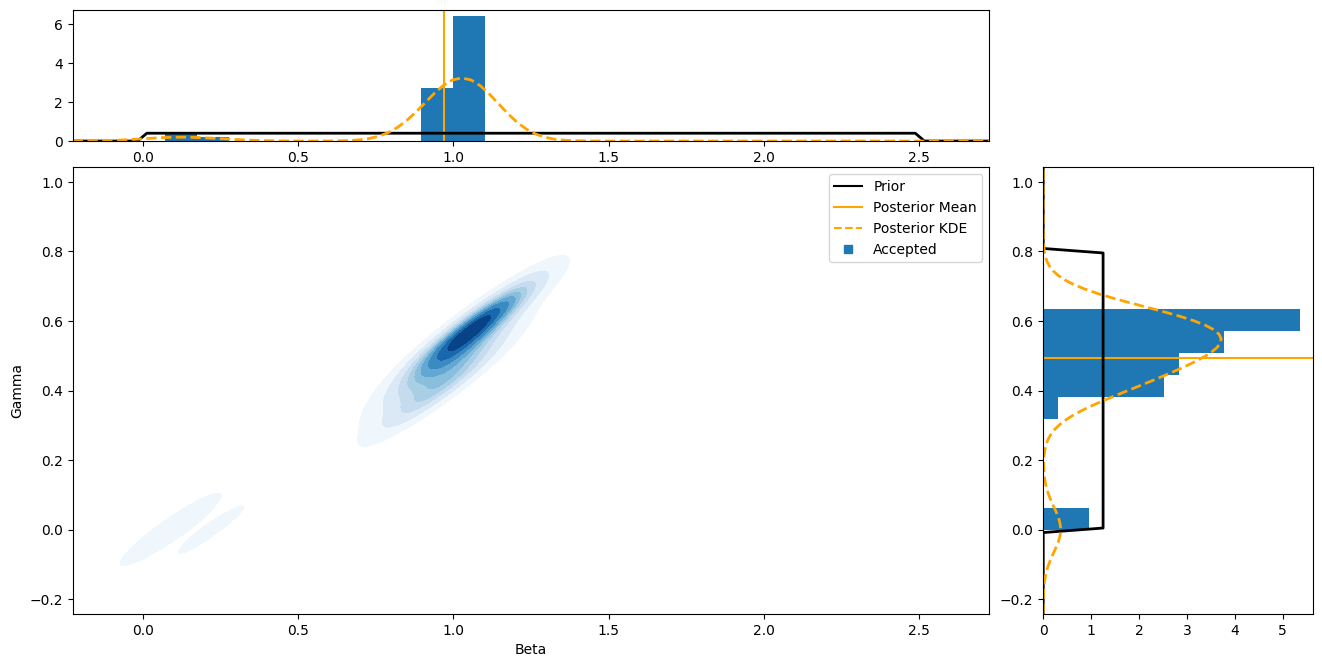
\includegraphics[width=\textwidth]{abc_rejection_joint_posterior_sir.PNG}
        \caption{"Best Samples" Rejection Sampling}
        \label{fig_joint_distribution_full_time_series_rejection}
      \end{subfigure}
      \begin{subfigure}{.45\paperwidth}
        \centering
        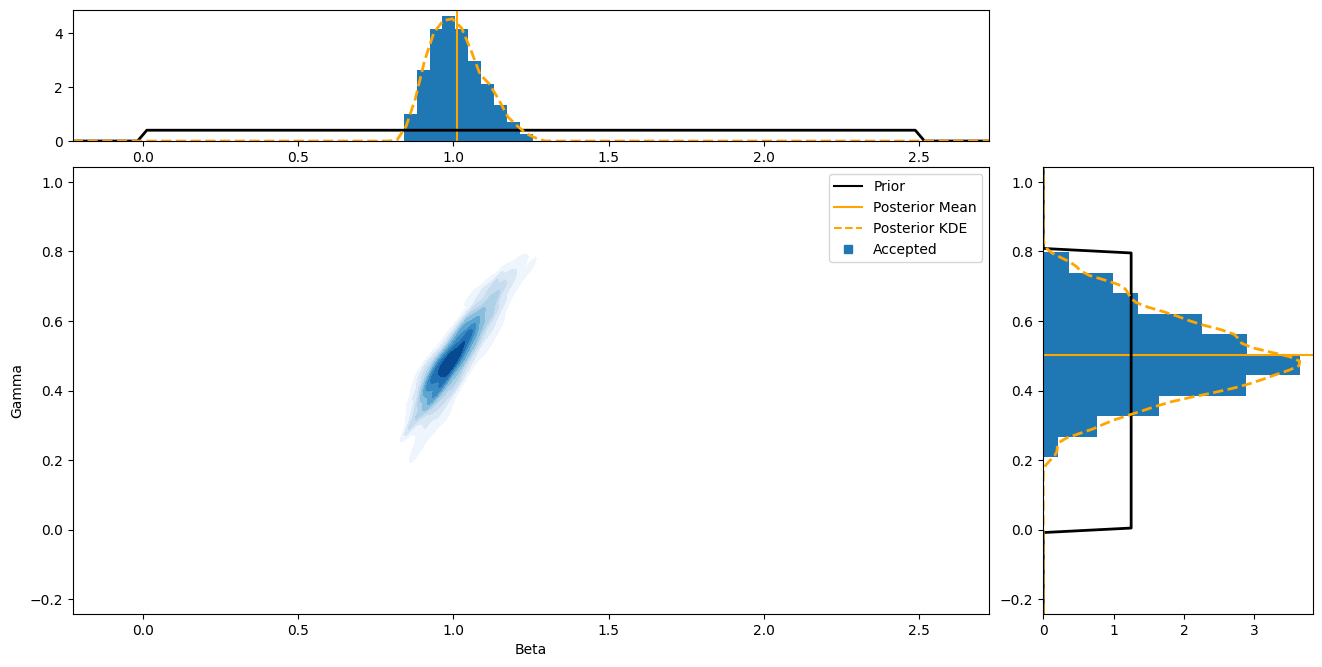
\includegraphics[width=\textwidth]{abc_mcmc_joint_posterior_sir.PNG}
        \caption{ABC-MCMC}
        \label{fig_joint_distribution_full_time_series_mcmc}
      \end{subfigure}
    }
    \makebox[\textwidth][c]{
      \begin{subfigure}{.45\paperwidth}
        \centering
        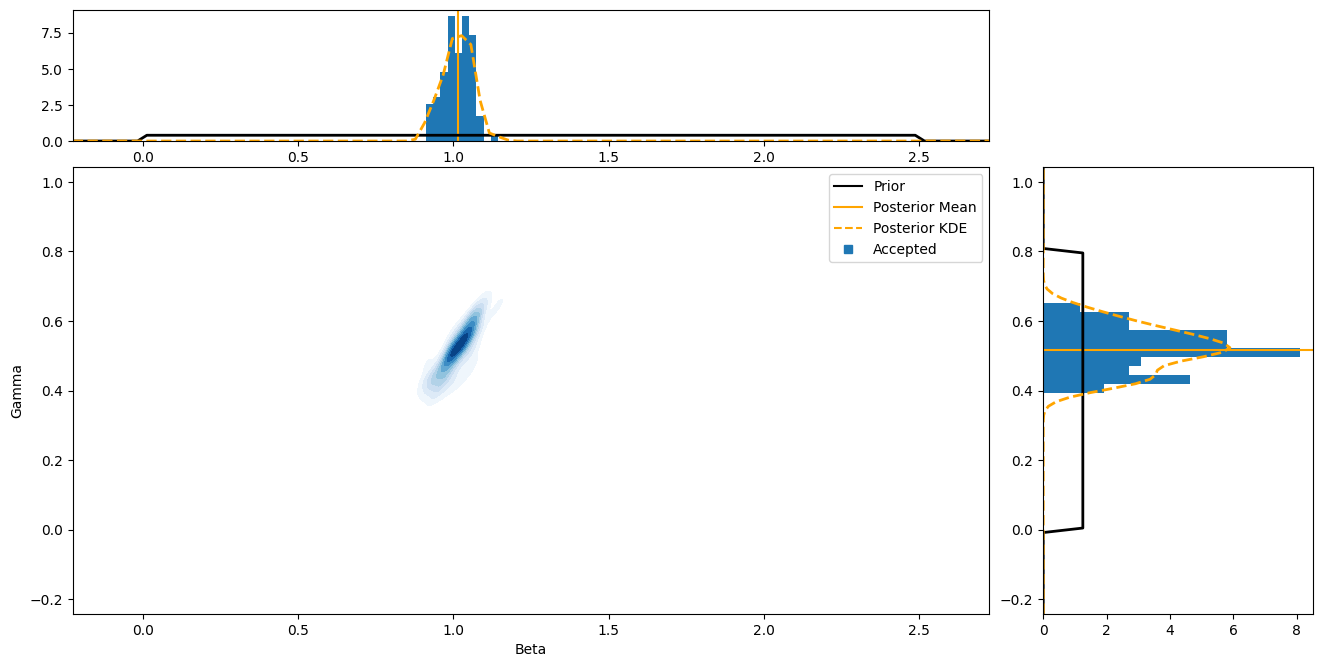
\includegraphics[width=\textwidth]{abc_smc_joint_posterior_sir.PNG}
        \caption{ABC-SMC}
        \label{fig_joint_distribution_full_time_series_smc}
      \end{subfigure}
      \begin{subfigure}{.45\paperwidth}
        \centering
        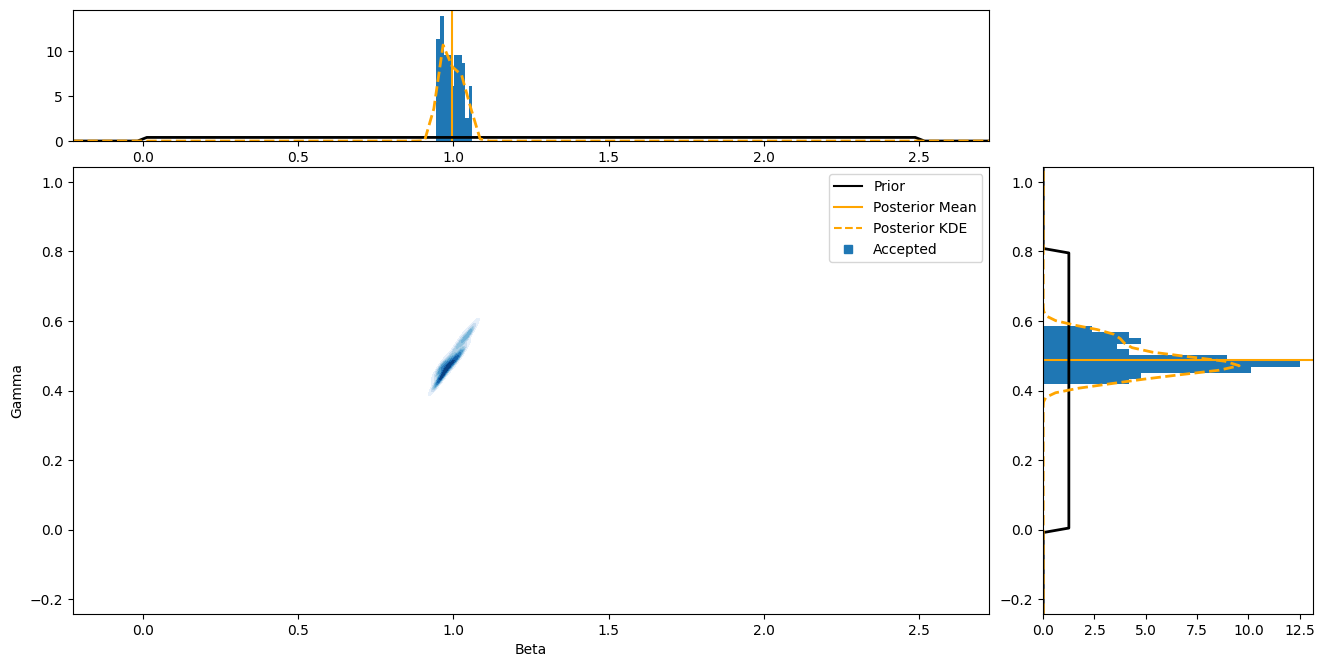
\includegraphics[width=\textwidth]{abc_adaptive_smc_joint_posterior_sir.PNG}
        \caption{Adaptive ABC-SMC}
        \label{fig_joint_distribution_full_time_series_adaptive_smc}
      \end{subfigure}
    }
    \caption{Joint and marginal posterior distributions of $\beta$, horizontal axis, and $\gamma$, vertical axis, parameters generated by different ABC-methods when provided with the full time-series of data.}
    \label{fig_joint_distribution_full_time_series}
  \end{figure}

  The first experiment ran each algorithm 50 times on the full time-series data, with the configurations described above. \textit{Table \ref{table_abc_methods_on_sir_model}} provides a summary of these results and \textit{Figure \ref{fig_joint_distribution_full_time_series}} provides the marginal and joint posteriors returned by each algorithm.

  \par It is apparent from the distributions in \textit{Figure \ref{fig_joint_distribution_full_time_series}} that all methods have achieved a significant level of learning as the priors (black) and estimated posteriors (blue/orange) are highly dissimilar. This is clear when you observe the plots of the joint distribution as the limits of the plot include the whole prior space but the vast majority of each plot is white, indicating effectively no posterior mass is placed in those regions. Moreover, each algorithm has estimated a posterior which significant posterior mass around the true parameter values.

  \begin{figure}[H]
    \centering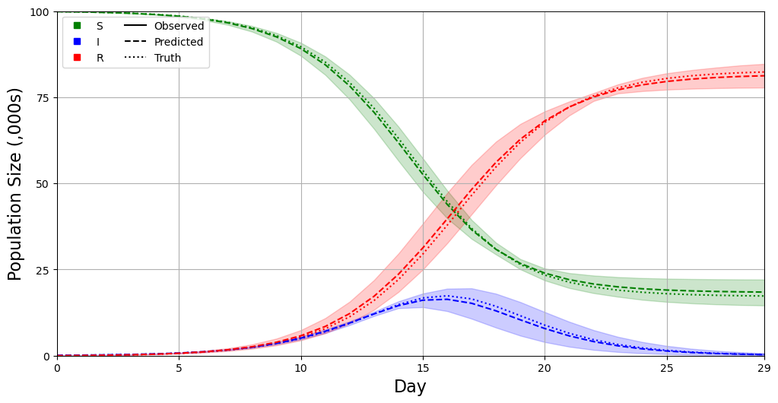
\includegraphics[width=.7\textwidth]{Semi_Auto_ABC_SMC_full_data_CI.png}
    \caption{95\% Confidence Intervals for model fitted to the SIR model described in \textit{Figure \ref{fig_example_standard_sir_model}} using adaptive ABC-SMC with ~5,000 simulations and the identity function as the summary statistic. 95\% confidence interval for $R_0$ is [1.784,2.266].}
    \label{fig_abc_smc_sir_identity_95_ci}
  \end{figure}

  \par The best fitting model is produced by the ABC-SMC algorithm (RSSE=2,393) with the Adaptive ABC-SMC producing only a slightly worse fit (RSSE=2,563, See \textit{Figure \ref{fig_abc_smc_sir_identity_95_ci}}) . This is highly encouraging for the Adaptive ABC-SMC algorithm as it requires significantly less tuning then all the other algorithms, except for ``Best Samples'' ABC-Rejection Sampling which does not perform nearly as well (RSSE=3,721). However, the Adaptive ABC-SMC algorithm took on average 4.24 times as long to be executed than the ABC-SMC algorithm. This is unsurprising as many of the first iterations of Adaptive ABC-SMC have almost a 100\% acceptance rate whilst the acceptance kernel bandwidth is still large. This high acceptance rate is inefficient as significant computation time occurs at the end of each step of the Adaptive ABC-SMC algorithm in order to calculate perturbance kernel variances and acceptance kernel bandwidths, meaning the average computation time per simulation is notably greater early on in the algorithms run.

  \par By inspecting \textit{Table \ref{table_abc_methods_on_sir_model}} we can note that all the algorithms produce 95\% confidence intervals which include the true value of both model parameters. The confidence intervals produced for $\beta$ are notably tighter than those produced for $\gamma$ in all cases except for ``Best Samples'' ABC-Rejection Sampling. This is surprising as the magnitude of $\beta$ is greater than that of $\gamma$ so we would expect small changes in $\gamma$ to have a greater affect on the resulting model fit. This is likely a result of the peak of infections occurring in the later half of the time-series (day 17 of 30) and thus there being more days in which infections are increasing.

  \begin{figure}[H]
    \centering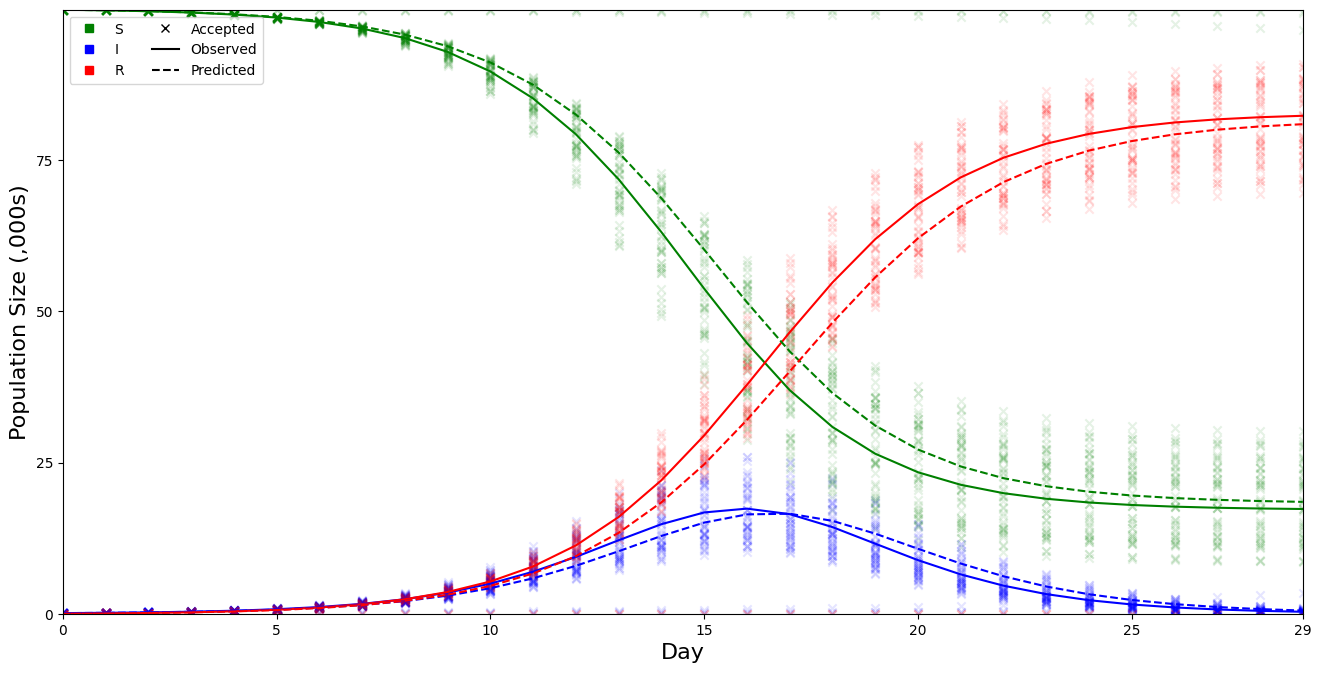
\includegraphics[width=.7\textwidth]{abc_rejection_accepted.png}
    \caption{The 1\% best generated samples which were accepted by ABC-Rejection Sampling (crosses) when given the full time-series and using the identity function as the summary statistic. Includes the observed data (solid line) and the data from a model fitted with the posterior mean values for each parameter (dashed line).}
    \label{fig_abc_rejection_accepted}
  \end{figure}

  \par The ``Best Samples'' ABC-Rejection Sampling algorithm is the only one to produce a bi-modal posterior. The majority of the estimated posterior mass is placed around the true values of the parameters, but a non-neglible amount is also placed around $(\beta,\gamma)=(0,0)$. This pair of parameter values is the unique case where no infections ever occur. \textit{Figure \ref{fig_abc_rejection_accepted}} plots all the simulated values which were accepted by a particular run of the ``Best Samples'' ABC-Rejection Sampling algorithm, along with the observed data (solid line) and the data generated by a model fitted with posterior means (dashed line). In \textit{Figure \ref{fig_abc_rejection_accepted}} we can clearly see these special cases where $(\beta,\gamma)\simeq(0,0)$ as their simulated values never leave the horizontal axes. This plot motivates the ability to set the acceptance rate of the ``Best Samples'' flavour of ABC-Rejection Sampling after all samples have been generated as we clearly see that these special cases will have distinctly greater distance values that the other accepted samples and thus would have just snuck into the top 1\% of samples. We can justify tightening the acceptance criteria to exclude these simulations as they are demonstrably incorrect.

\subsubsection*{Results - Experiment Two}

  \begin{table}[H]
    \centering
    \begin{tabular}{|l|l|}
      \hline
      \textbf{Algorithm}&\textbf{LOO-CV Score}\\\hline\hline
      ``Best Samples'' ABC-Rejection Sampling&6,135\\\hline
      ABC-Importance Sampling&5,001\\\hline
      ABC-MCMC&3,023\\\hline
      ABC-SMC&643\\\hline
      Adaptive ABC-SMC&439\\\hline
    \end{tabular}
    \caption{Leave-One-Out Cross-Validation Scores for different ABC algorithms when applied to the SIR model described in \textit{Figure \ref{fig_example_standard_sir_model}}. Each algorithm performed approximately 5,000 simulations each iteration, had rough tuning to achieve appropriate acceptance rates and used the identity function as the summary statistic.}
    \label{table_abc_methods_on_sir_model_loo_cv}
  \end{table}

  \par The second experiment assessed the general performance of the ABC methods when applied to standard SIR models by performing a leave-one-out cross-validation of each algorithm. A leave-one-out cross-validation was performed on each algorithm when applied to the SIR model depicted in \textit{Figure \ref{fig_example_standard_sir_model}}, with each algorithm configured as described at the start of this section. The score of each algorithm is given in \textit{Table \ref{table_abc_methods_on_sir_model_loo_cv}}.

  \par The Adaptive of ABC-SMC achieves the lowest LOO-CV score, suggesting it performs the best in general scenarios. This is unsurprising as each iteration of the cross-validation sees a different piece of data missing and thus the optimal configuration of the hyper-parameters will be different each time. As Adaptive ABC-SMC automatically updates the majority of its hyper-parameters it should perform well in this test, and does.

  \par The difference in scores between each algorithm in \textit{Table \ref{table_abc_methods_on_sir_model_loo_cv}} than in \textit{Table \ref{table_abc_methods_on_sir_model}}, when the full time-series was supplied to each algorithm. This demonstrates the effect that tuning of parameters has on the performance of each algorithm.

  \par A closer inspection of the results from the cross-validation showed that the majority (40-60\%) of the total error from each algorithm occurred when one of the data-points from days 14-18 was removed. This is due to these days coincide with the peak-infectious population size which is a key point in the lifespan of an epidemic and is the point at which more information is available about parameter $\beta$ than $\gamma$.

\subsection{Comparison of Summary Statistic Methods}\label{sec_comparison_of_ss_methods}

  \par \textit{Section \ref{sec_summary_stats}} presented four methods for automating the process of choosing summary statistics for ABC-methods: Approximately Sufficient Subset (ASS); Minimum Entropy (ME); Two-Step Minimum Entropy (2-ME); and, Semi-Automatic ABC (SA-ABC). Here I assessed these algorithms by running 50 instances of each algorithm; Running the Adaptive ABC-SMC algorithm, for 5,000 simulations, using the most recommended set of summary statistics from each algorithm; and then calculating the mean-square error produced by a model fitted with the estimated posterior mean of each parameter.

  \begin{table}[H]
    \centering
    \begin{framed}
      {\small
        \begin{multicols}{2}
          \begin{enumerate}[label=(S\arabic*)]
            \item *Peak size of infectious population (1).\label{table_list_of_summary_statistics_peak_size}
            \item Date of peak infectious population (1).\label{table_list_of_summary_statistics_peak_date}
            \item *Final size of susceptible population (1).\label{table_list_of_summary_statistics_final_sus}
            \item *Final size of infectious population (1).
            \item *Final size of removed population (1).
            \item *Mean size of susceptible population (1).
            \item *Mean size of infectious population (1).\label{table_list_of_summary_statistics_mean_inf}
            \item *Mean size of removed population (1).\label{table_list_of_summary_statistics_mean_rem}
            \item *Maximum day-on-day increase in infectious population (1).
            \item *Maximum day-on-day increase in removed population (1).
            \item *Population sizes on days 1,\dots,30 as different statistics (3).\label{table_list_of_summary_statistics_daily}
            \item *Net weekly change in susceptible population (4).
            \item *Net weekly change in infectious population (4).
            \item *Net weekly change in removed population (4).
            \item *Net daily change in susceptible population (29).
            \item *Net daily change in infectious population (29).
            \item *Net daily change in removed population (29).
            \item *Cummulative sum of daily susceptible population (29).
            \item *Cummulative sum of daily infectious population (29).
            \item *Cummulative sum of daily removed population (29).
            \item Uniform random variable in [10,22] (1).\label{table_list_of_summary_statistics_random}
            \item Constant mapping to 16 $s(x)=16$ (1).\label{table_list_of_summary_statistics_constant}
          \end{enumerate}
        \end{multicols}
      }
    \end{framed}
    \caption{Comprehensive set of 99 summary statistics supplied to the ASS, ME and 2-ME algorithms. An asterisk (*) denotes that a summary statistic of the natural logarithm of this value was supplied as well. In brackets is the dimensionality of each summary statistic when applied to the SIR-model depicted in \textit{Figure \ref{fig_example_standard_sir_model}} which runs for 30 time-periods.}
    \label{table_list_of_summary_statistics}
  \end{table}

  \par Three of the algorithms presented in \textit{Section \ref{sec_summary_stats}} (ASS,ME and 2-ME) choose an optimal set of summary statistics from a larger set. \textit{Table \ref{table_list_of_summary_statistics}} provides the set of summary statistics supplied to these algorithms. (\ref{table_list_of_summary_statistics_peak_size},\ref{table_list_of_summary_statistics_peak_date}) are taken from \cite[]{hiv_with_contact_tracing} which found the peak size of the infectious population and the date on which this peak occurred to be the best performing summary statistics when applied to data regarding HIV in Cuba\footnote{It is noteworthy that they were working with yearly data, so this result may be less applicable to data collected at shorter intervals.}. (\ref{table_list_of_summary_statistics_random},\ref{table_list_of_summary_statistics_constant}) are totally uninformative and were supplied to test whether the algorithms would ever choose such summary statistics. These two summary statistics were specified to both have an expected value of 16 so that they coincide with (\ref{table_list_of_summary_statistics_peak_date}) for the true model.

  \par All four algorithms were configured to use the log-Euclidean distance (\ref{eqn_log_euclidean_distance}). The ASS algorithm was configured to generate 100,000 simulations and to use a Gaussian acceptance kernel with bandwidth .5. These simulations and kernel were used to determine which sets of parameters to accept for each set of summary statistics, and these sets were then supplied to \textit{Algorithm \ref{alg_evaluate_proposed_statistic}} in order to determine whether to accept the newly proposed summary statistic.

  \par Algorithm ME was configured to generate 100,000 simulations from which the best 1,000 were chosen (using ``Best Samples'' ABC-Rejection Sampling) and entropy estimated from. Algorithm 2-ME was configured to run ME, as just described, to identify the initial set of summary statistics $S_{ME}$ and to retain the best 100 simulations $\hat\Theta_{ME}$ according to $S_{ME}$. 100,000 fresh simulations were then generated and the 1,000 best simulations $\Theta_{acc}$ were identified for each set of summary statistics (using ``Best Samples'' ABC-Rejection Sampling) and the MRSSE was calculated between $\Theta_{acc}$ and $\hat\Theta_{ME}$. For time-tractability both algorithms were restricted to only considering subsets of summary statistics up to size four, this still involved the consideration of 92,170 different subsets\footnote{(\ref{table_list_of_summary_statistics_daily}) were removed from the set of possible summary statistics for these two algorithms as it represents 60 unique summary statistics and thus would bring the total number of sets up to size four to 3,926,175.}.

  \par The pilot posterior $f_{\theta}$ for SA-ABC was generated by ``Best Samples'' ABC-Rejection Sampling using the identity function and retaining the best 1,000 of a set of 100,000 simulations. 5,000 sets of parameters were then generated from the pilot posterior $f_\theta$ and used in the regression to calculate the summary statistics. As the SIR model has two parameters SA-ABC generates a summary statistic with two dimensions.

  \par To compare the performance of each algorithm I ran each algorithm 50 times and identified the most commonly returned set of statistics. Adaptive ABC-SMC\footnote{Adaptive ABC-SMC was used as it performed best in the general setting in \textit{Section \ref{sec_comparison_of_abc_methods}}. Adaptive ABC-SMC was configured as described in \textit{Section \ref{sec_comparison_of_abc_methods}} so that the results from \textit{Table \ref{table_abc_methods_on_sir_model}} can be used as a benchmark.}. was then run 50 times with each set of statistics and the average MSE was calculated between models fitted with the estimated posterior means and the true model. I chose to only calculate the MSE for the most commonly returned set of statistics, rather than for each set of returned statistics and taking the mean, as each the tested methods only takes a few minutes to run and thus it is reasonable to run each algorithm many times. Moreover, for each algorithm there was a set of statistics which was chosen significantly more often than any other.

\subsubsection*{Results}

  \begin{table}[H]
    % \centering
    \begin{tabular}{|l|l|l|l|}
      \hline
      \textbf{Algorithm}&\textbf{Returned Statistics}&\textbf{Dimensions}&\textbf{\% Runs Returned}\\
      \hline \hline
      Control&Identity Function&90&N/A\\\hline
      Approximately Sufficient&[Log-Final Susceptible Population (\ref{table_list_of_summary_statistics_final_sus}*)]&1&44\%\\
       Subset&&&\\\hline
      Minimum Entropy&[Log-Mean Infectious Population (\ref{table_list_of_summary_statistics_mean_inf}*),&2&30\%\\
      &Log-Mean Removed Population (\ref{table_list_of_summary_statistics_mean_rem}*)]&&\\\hline
      2-Step ME&[Log-Peak Infectious Population Size (\ref{table_list_of_summary_statistics_peak_size}*),&3&34\%\\
      &Log-Mean Infectious Population (\ref{table_list_of_summary_statistics_mean_inf}*),&&\\
      &Log-Mean Removed Population (\ref{table_list_of_summary_statistics_mean_rem}*)]&&\\\hline
      Semi-Automatic ABC&N/A&2&N/A\\\hline
    \end{tabular}\\
    \bigskip
    \begin{tabular}{|l|l|l|}
      \hline
      \textbf{Algorithm}&\textbf{ABC-SMC MSE}&\textbf{Time (s)}\\
      \hline \hline
      \textit{Control}&121,777&N/A\\\hline
      Approximately Sufficient Subset&101,730,336&25\\\hline
      Minimum Entropy&1,131,712&150\\\hline
      2-Step ME&228,150&302\\\hline
      Semi-Automatic ABC&643,255&102\\\hline
    \end{tabular}\\

    \caption{The most commonly returned set of summary statistics returned by each algorithm and the mean square error when using Adaptive ABC-SMC to fit the SIR model described in \textit{Figure \ref{fig_example_standard_sir_model}} with said set of statistics. Additionally, the dimensionality of each summary statistic when applied to the SIR-model depicted in \textit{Figure \ref{fig_example_standard_sir_model}}; the percentage of instances in which this set of statistics was returned; and, the mean runtime of each selection algorithm are given. All values are the means over 50 instances of each selection algorithm. Note that in all cases the natural logarithm version of a summary statistic was chosen, rather than its raw value.}
    \label{table_summary_selection_methods_on_sir_model}
  \end{table}

  \par \textit{Table \ref{table_summary_selection_methods_on_sir_model}} provides the summary of the results of running each selection algorithm 50 times and then running Adaptive ABC-SMC with the most commonly returned set of statistics. None of the returned set of statistics performs as well as the identity function, although it would be very surprising if this was the case. Both 2-ME and SA-ABC returned sets of summary statistics which produced MSE of the same order of magnitude as the identity function despite only having 3 and 2 dimensions, respectively, compared to the 90 of the identity function. The ASS algorithm performs very poorly, this is likely due to difficulties in implementation which mean it heavily favours low dimension summary statistics. ME produces a well performing set of summary statistics, but it is notably slower and produces a greater MSE than SA-ABC. It is noteworthy that 2-ME returns a set of summary statistics which is a superset of those returned by ME. This indicates that the second step of 2-ME does draw more nuance than ME, the motivation behind adding the second step.

  \par These results demonstrate that their are methods for selecting summary statistics which produce summary statistics which perform similarly to the identity function despite having significantly fewer dimensions. Moreover, if these algorithms were supplied with more simulations then we can expect for the difference in performance between the identity function and generated summary statistics to decrease. This is more relevant to SA-ABC as each extra simulation means its regression step is more informed, while 2-ME can only ever return a set of statistics from a predefined set and thus more simulations would only make its returned results more consistent.

  \par None of the algorithms returned the same set of summary statistics a majority of the time. An inspection of the distribution of returned sets shows that the sets given in \textit{Table \ref{table_summary_selection_methods_on_sir_model}} were all accepted as least 3 times more often than the next most commonly returned sets. If the algorithms were given more simulations then this ratio should increase as the estimated values (i.e. entropy) will tend towards their true value, by the law of large numbers.

  \begin{figure}[H]
    \centering
    \makebox[\textwidth][c]{
      \begin{subfigure}{.45\paperwidth}
        \centering
        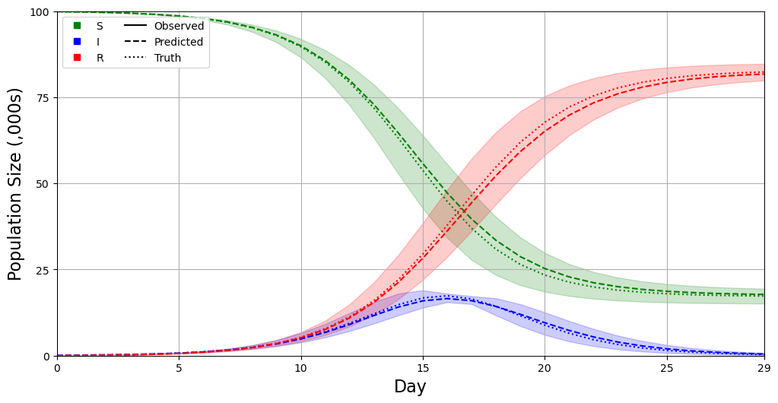
\includegraphics[width=\textwidth]{two_step_ME_ABC_SMC_full_data_CI.PNG}
        \caption{Two-Step Minimum Entropy. 95\% confidence interval for $R_0$ is [1.957,2.073].}
        \label{fig_summary_statistic_selected_by_two_step_me}
      \end{subfigure}
      \begin{subfigure}{.45\paperwidth}
        \centering
        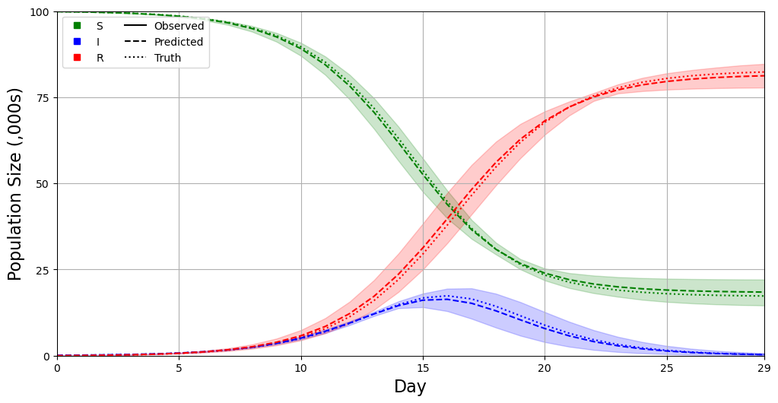
\includegraphics[width=\textwidth]{Semi_Auto_ABC_SMC_full_data_CI.PNG}
        \caption{Semi-Automatic ABC. 95\% confidence interval for $R_0$ is [1.754,2.132].}
        \label{fig_summary_statistic_selected_by_semi_auto}
      \end{subfigure}
    }
    \caption{95\% CI when running adaptive ABC-SMC using summary statistics generated by two-step minimum entropy and semi-automatic ABC respectively.}
    \label{fig_compare_summary_statistic_selections}
  \end{figure}

  \textit{Figure \ref{fig_compare_summary_statistic_selections}} provides plots of the 95\% confidence intervals for each population size produced by ABC-SMC when using the summary statistics returned by 2-ME (\ref{fig_summary_statistic_selected_by_two_step_me}) and SA-ABC (\ref{fig_summary_statistic_selected_by_semi_auto}). (See \textit{Figure \ref{fig_abc_smc_sir_identity_95_ci}} for the results when the identity function is used). A notable difference between the two plots its their confidence around the peak of the infection, with 2-ME having much more concentrated certainty around the true peak than SA-ABC. This is due to the set of statistics returned by 2-ME including the logarithm of the peak number of infections. Moreover, \textit{Figure \ref{fig_summary_statistic_selected_by_semi_auto}} perfectly fits the infectious population until the peak is reached at which point it typically expected the peak to occur later than it actually does.

  \par This difference in the resulting fit of the two sets of summary statistics suggests that different selection algorithms should be used for different inference problems. With SA-ABC being best suited for general problems regarding the full time-series, whilst 2-ME is better when you have a specific problem (e.g. will hospitals be over-run when the peak of infections occurs) as you can supply it summary statistics which it is reasonable to expect to perform well for this problem (e.g. (\ref{table_list_of_summary_statistics_peak_size},\ref{table_list_of_summary_statistics_peak_date}) for problems regarding peak infections).

\subsection{The Effect of Dimensionality}\label{sec_effect_of_dimensionality}

  Plot dimensionality of summary stats against MSE (use ME to choose best at each dimensionality)

  \begin{table}[H]
    \centering
    \begin{tabular}{|l|l|l|l|}
      \hline
      \textbf{Dimensions}&\textbf{Best Stats}&\textbf{Estimated Entropy}&\textbf{ABC-SMC MSE}\\\hline
      1&[Mean Susceptible Population]&-9.48&2,272,479\\\hline
      2&[Mean Infectious Population,&-10.74&1,131,712\\
      &Mean Removed Population]&&\\\hline
      3&[Final Removed Population,&-10.59&1,540,652\\
      &Mean Infectious Population,&&\\
      &Mean Removed Population]&&\\\hline
      4&[Net Weekly Change in Removed Population]&-10.60&756,888\\\hline
      90&Identity Function&-11.70&756,888\\\hline
    \end{tabular}
    \caption{The best summary statistics at each dimensionality according to the minimum entropy algorithm, along with their estimated entropy values and mean square error.}
    \label{table_dimensionality_of_summary_statistics}
  \end{table}

\subsection{Projection}\label{sec_projection}

  \begin{figure}[H]
    \centering
    \makebox[\textwidth][c]{
      \begin{subfigure}{.45\paperwidth}
        \centering
        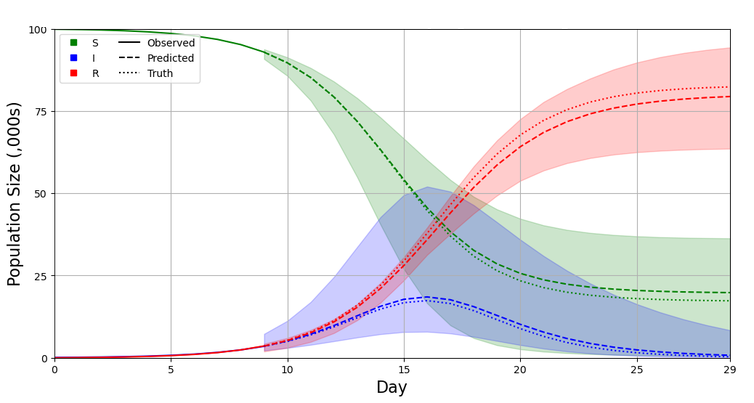
\includegraphics[width=1\textwidth]{Semi_Auto_ABC_SMC_10_days_CI.png}
        \caption{First 10 days of data given. 95\% CI for $R_0$ is [1.583,2.767.]}
        \label{fig_semi_auto_10_days}
      \end{subfigure}
      \begin{subfigure}{.45\paperwidth}
        \centering
        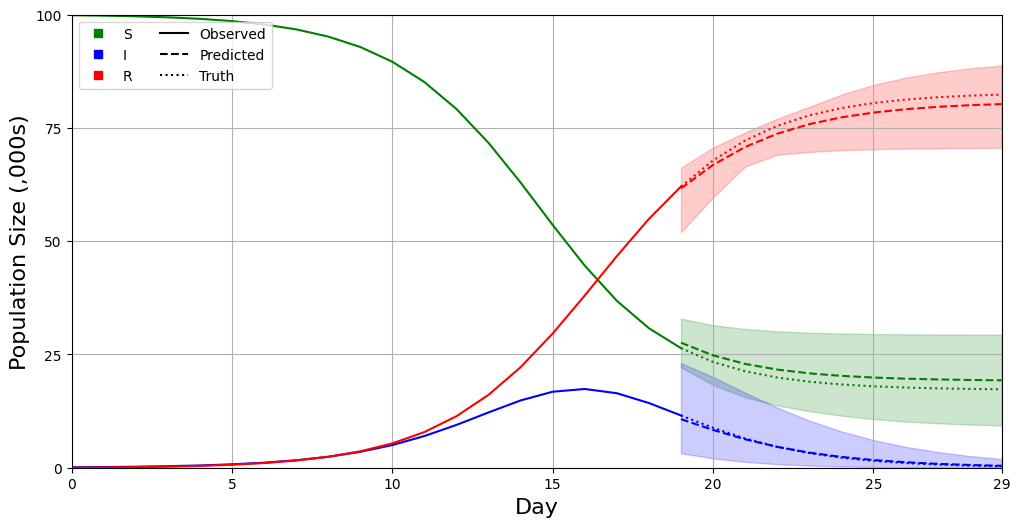
\includegraphics[width=1\textwidth]{Semi_Auto_ABC_SMC_20_days_CI.png}
        \caption{First 20 days of data given. 95\% CI for $R_0$ is [1.742,2.456].}
        \label{fig_semi_auto_20_days}
      \end{subfigure}
    }
    \makebox[\textwidth][c]{
      \begin{subfigure}{.45\paperwidth}
        \centering
        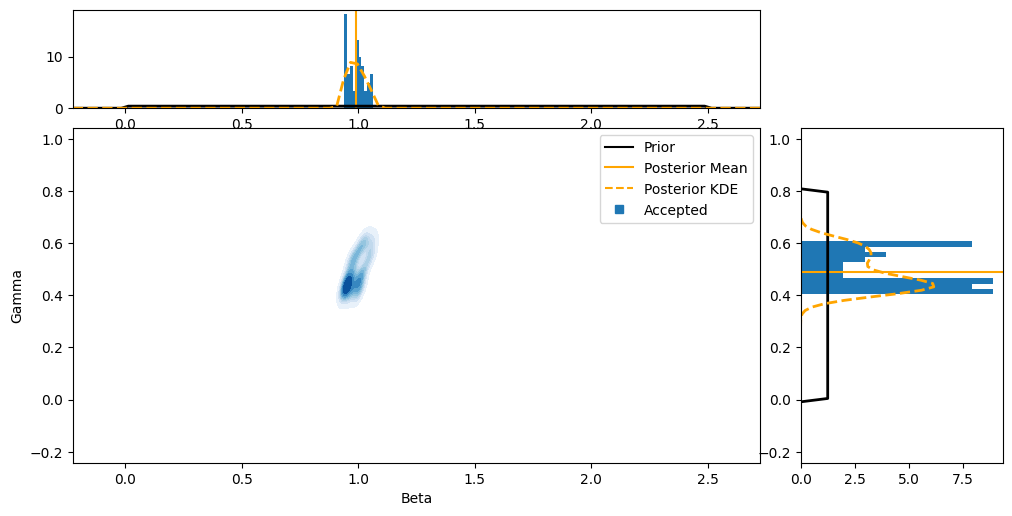
\includegraphics[width=1\textwidth]{Semi_Auto_ABC_SMC_10_days_joint_posterior.png}
        \caption{Posterior when first 10 days of data given. 95\% CI for $\beta$ is \text{[0.842,1.160]} and for $\gamma$ is \text{[0.305,0.705]}}
        \label{fig_semi_auto_10_days_posterior}
      \end{subfigure}
      \begin{subfigure}{.45\paperwidth}
        \centering
        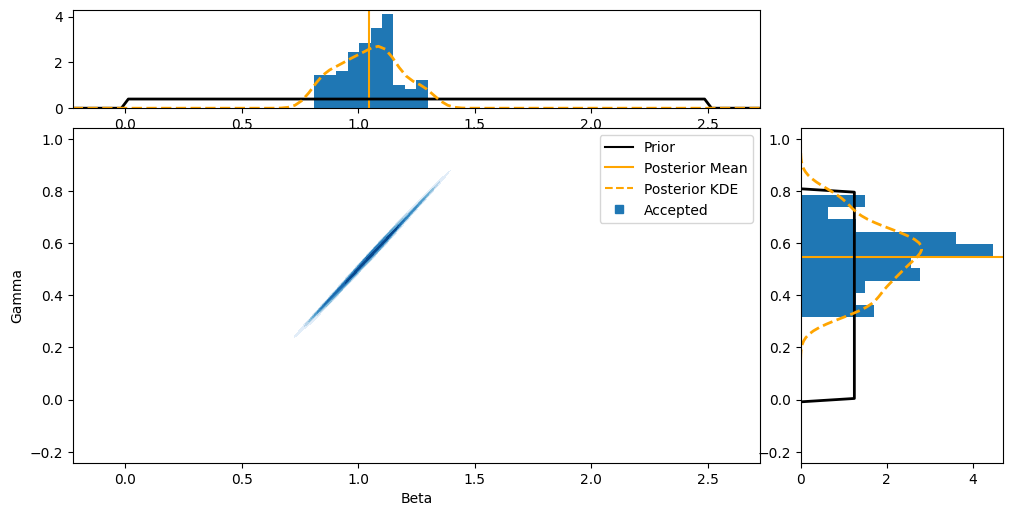
\includegraphics[width=1\textwidth]{Semi_Auto_ABC_SMC_20_days_joint_posterior.png}
        \caption{Posterior when first 20 days of data given. 95\% CI for $\beta$ is \text{[0.891,1.164]} and for $\gamma$ is \text{[0.340,0.603]}}
        \label{fig_semi_auto_20_days_posterior}
      \end{subfigure}
    }
    \caption{95\% CI when running adaptive ABC-SMC using summary statistics generated by semi-automatic ABC with only the first 10 or 20 days of data available. Accompanied by the estimated marginal and joint posteriors for the model parameters.}
    \label{fig_semi_auto_restricted_data}
  \end{figure}

\subsection{Real Data: France Covid-19}\label{sec_real_data}

  %https://www.medrxiv.org/content/10.1101/2020.04.26.20081042v1.full.pdf

\subsection{Real Data: Senegal Covid-19}\label{sec_real_data}

  %https://www.medrxiv.org/content/10.1101/2020.04.26.20081042v1.full.pdf

  \par Priors $\pi_{0,\beta}\sim\mathcal{U}(0,0.5),\ \pi_0{0,\gamma}\sim\mathcal{U}(.01,.1)$

  \par Rejection Sampling = 500,000 simulations and keep best 500. (5 minutes)
  \par Adaptive ABC-SMC = 5000 simulations, $\alpha=.9$ (26 minutes)
  \par Semi-Auto = 500,000 simulations, keep 100, generate 5,000 (dim=2)
  \par ME = 10,000 simulations per set, keep 100, max-size=4. Chose=[final\_removed\_ss,net\_weekly\_infections\_ss] (dim=5)
  \par 2-ME = Same as ME

  \begin{figure}[H]
    \centering
    \makebox[\textwidth][c]{
      \begin{subfigure}{.45\paperwidth}
        \centering
        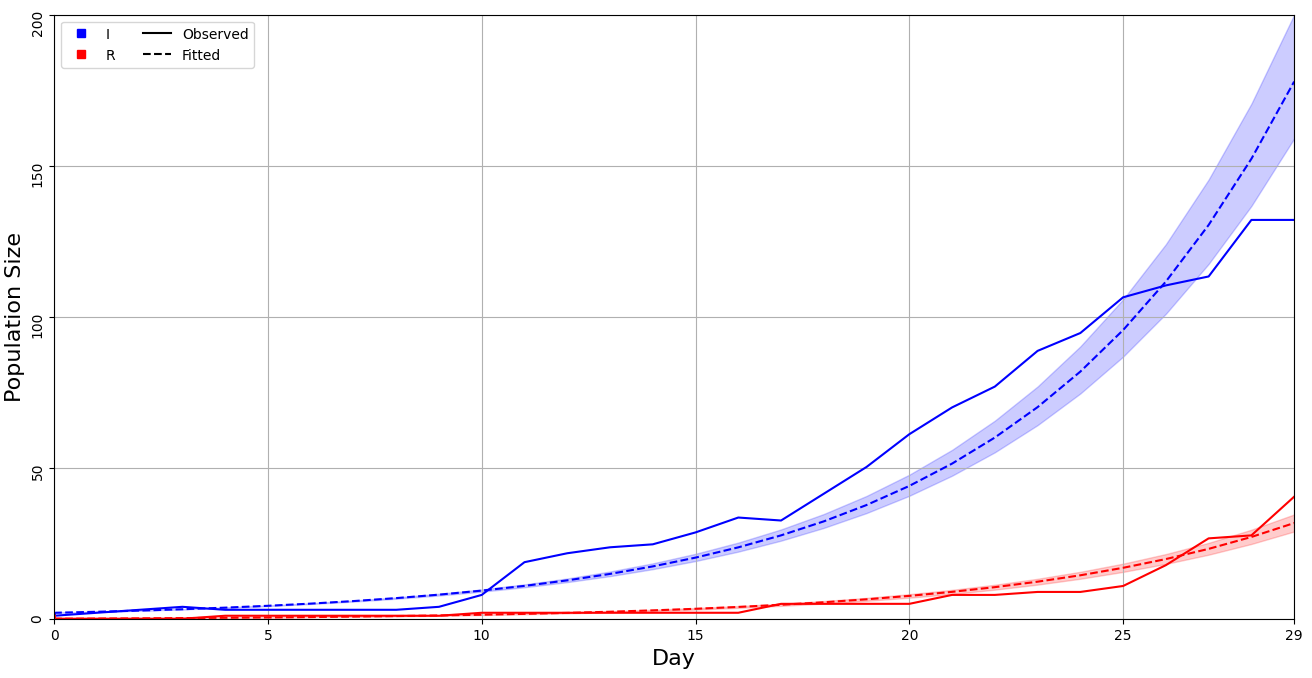
\includegraphics[width=\textwidth]{senegal_abc_rejection_identity_ci.PNG}
        \caption{"Best Samples" ABC-Rejection Sampling. 95\% CI for $R_0=[5.996,7.172]$. RSSE=316.}
        \label{fig_senegal_identity_ci_rejection_ci}
      \end{subfigure}
      \begin{subfigure}{.45\paperwidth}
        \centering
        % TODO redo vertical axes on confidence interval plots
        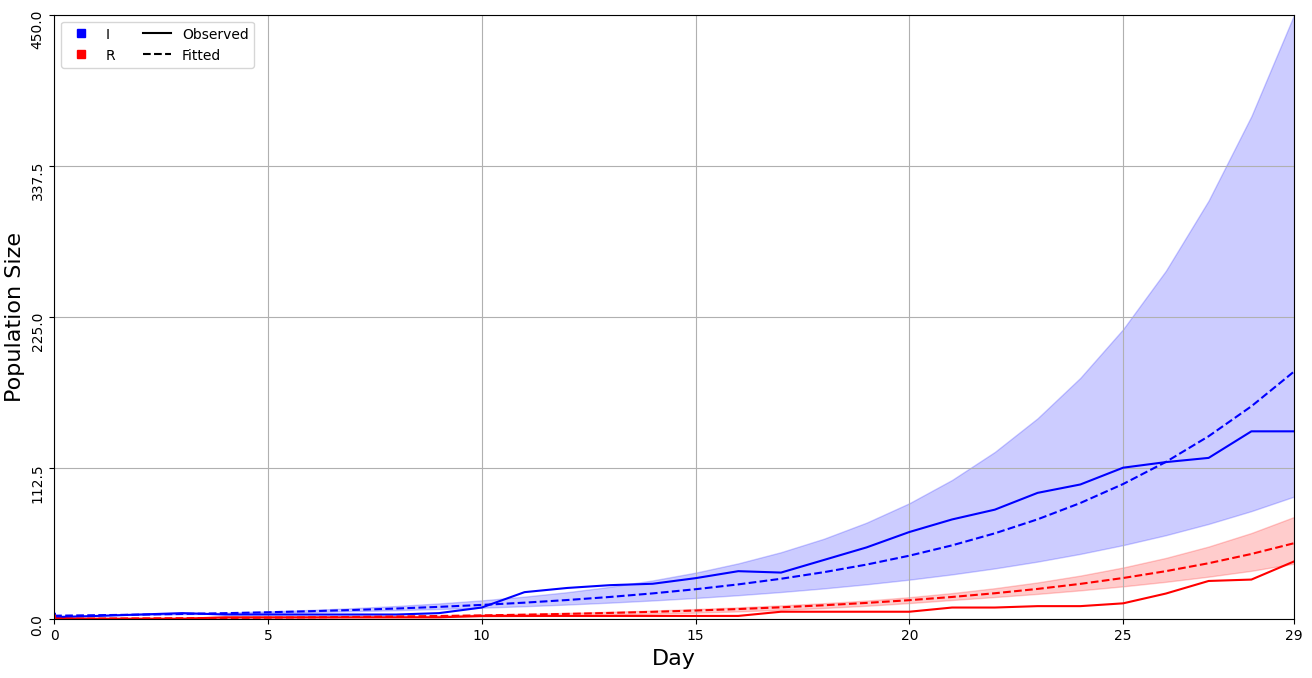
\includegraphics[width=\textwidth]{senegal_adapt_abc_smc_identity_ci.PNG}
        \caption{Adaptive ABC-SMC. 95\% CI for [3.160,8.107]. RSSE=376.}
        \label{fig_senegal_identity_ci_adapt_abc_smc}
      \end{subfigure}
    }
    \caption{95\% confidence intervals for infectious (blue) and removed (red) populations for Covid-19 in Senegal between March 2nd 2020 and March 31st 2020 using ``Best Samples'' ABC-Rejection Sampling and Adaptive ABC-SMC respectively. Both methods use the Log-Euclidean distance as their distance measures and the identity function of the infectious and removed populations as their summary statistic. The size of the susceptible population is not considered.}
    \label{fig_senegal_identity_ci}
  \end{figure}

  \begin{figure}[H]
    \centering
    \makebox[\textwidth][c]{
      \begin{subfigure}{.45\paperwidth}
        \centering
        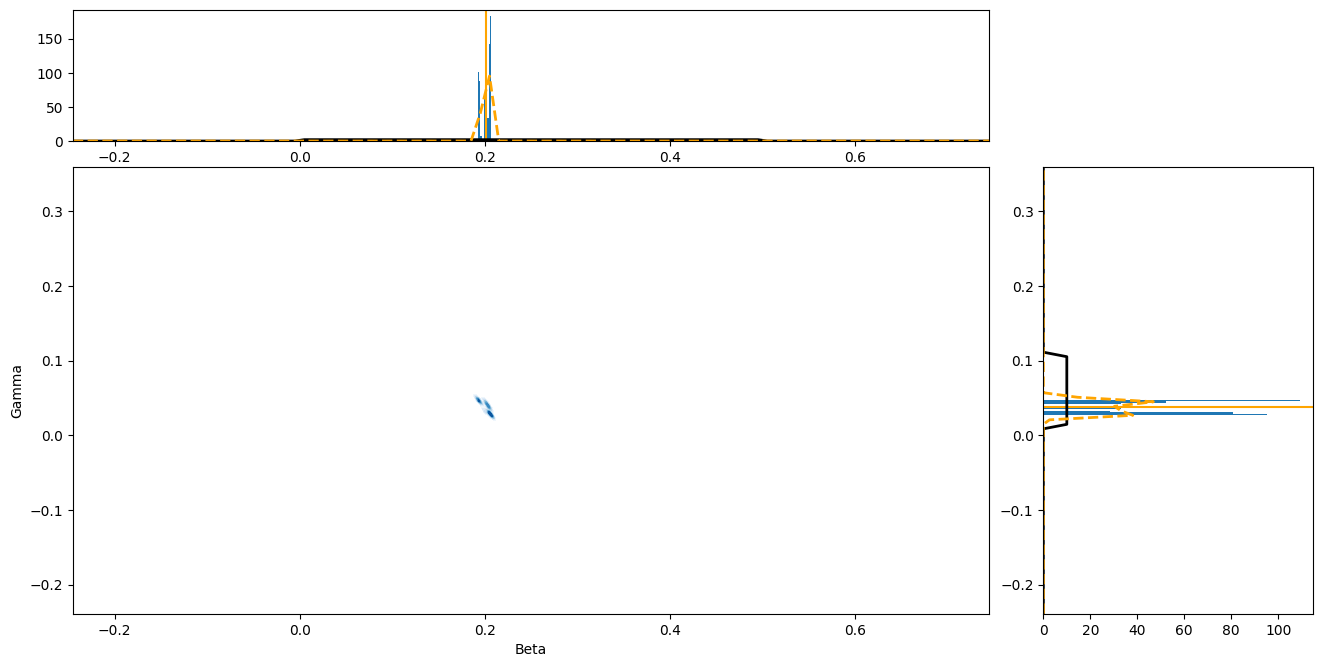
\includegraphics[width=\textwidth]{senegal_me_adapt_abc_smc_posterior.PNG}
        \caption{Joint and marginal posteriors for $\beta$ and $\gamma$.}
        \label{fig_senegal_me_posterior}
      \end{subfigure}
      \begin{subfigure}{.45\paperwidth}
        \centering
        % TODO redo vertical axes on confidence interval plots
        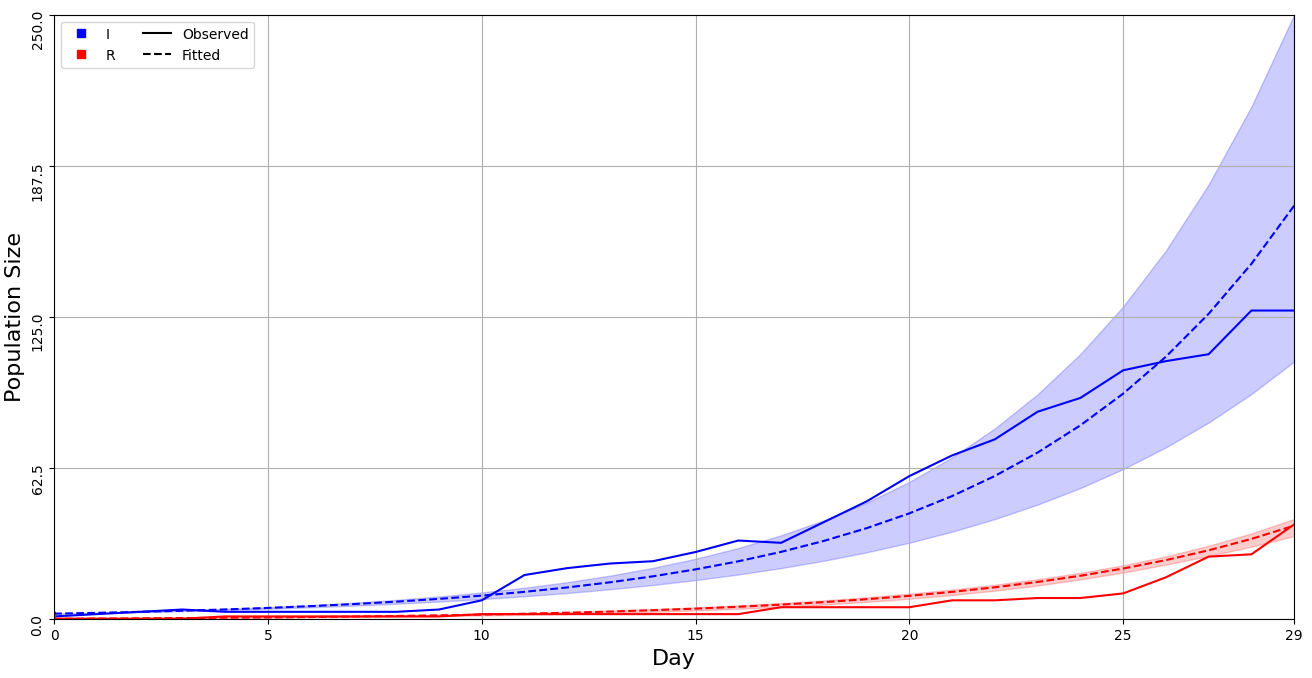
\includegraphics[width=\textwidth]{senegal_me_adapt_abc_smc_ci.PNG}
        \caption{95\% confidence intervals for population sizes. RSSE=324.}
        \label{fig_senegal_me_ci}
      \end{subfigure}
    }
    \caption{Estimated posteriors for SIR model parameters and resulting 95\% confidence intervals for the sizes of the infectious (blue) and removed (red) populations for Covid-19 in Senegal between March 2nd 2020 and March 31st 2020 when using Adaptive ABC-SMC with summary statistics generated by Minimum Entropy. 95\% CI for $R_0=[4.103,7.566],\ \beta=[0.185,0.211],\ \gamma=[0.049,0.012]$.}
    \label{fig_senegal_me}
  \end{figure}

  \begin{figure}[H]
    \centering
    \makebox[\textwidth][c]{
      \begin{subfigure}{.45\paperwidth}
        \centering
        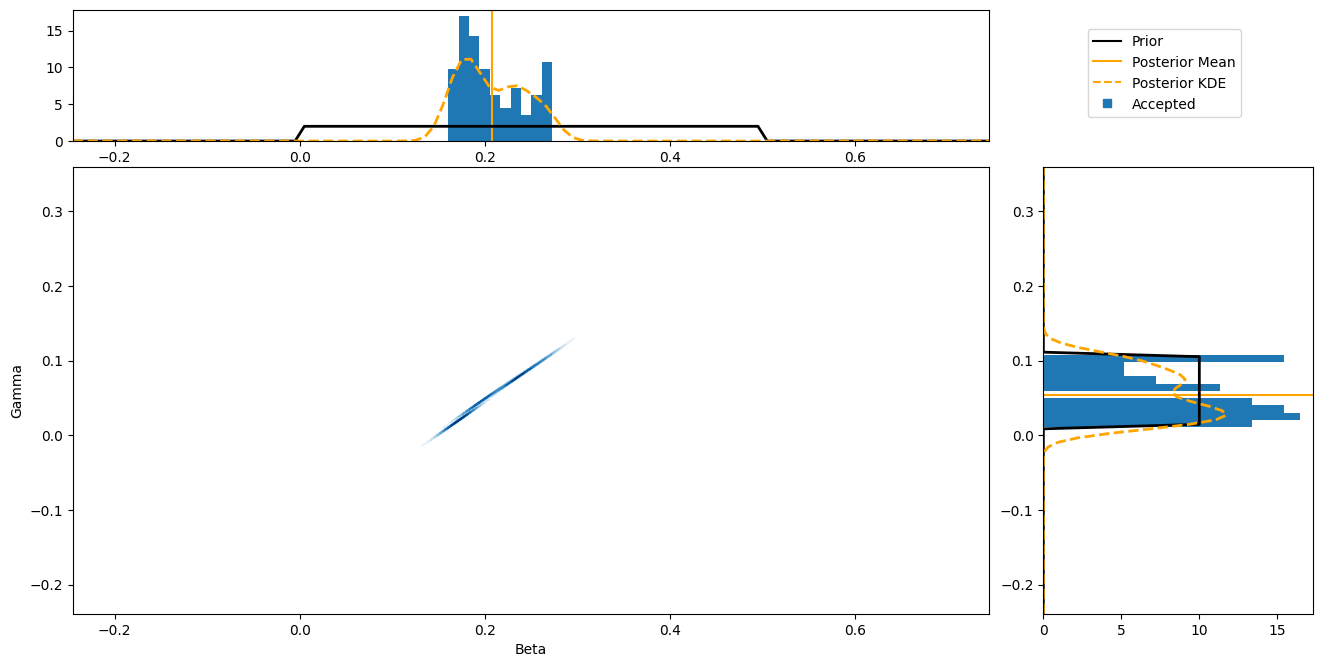
\includegraphics[width=\textwidth]{senegal_semi_auto_adapt_abc_smc_posterior.PNG}
        \caption{Joint and marginal posteriors for $\beta$ and $\gamma$.}
        \label{fig_senegal_semi_auto_posterior}
      \end{subfigure}
      \begin{subfigure}{.45\paperwidth}
        \centering
        % TODO redo vertical axes on confidence interval plots
        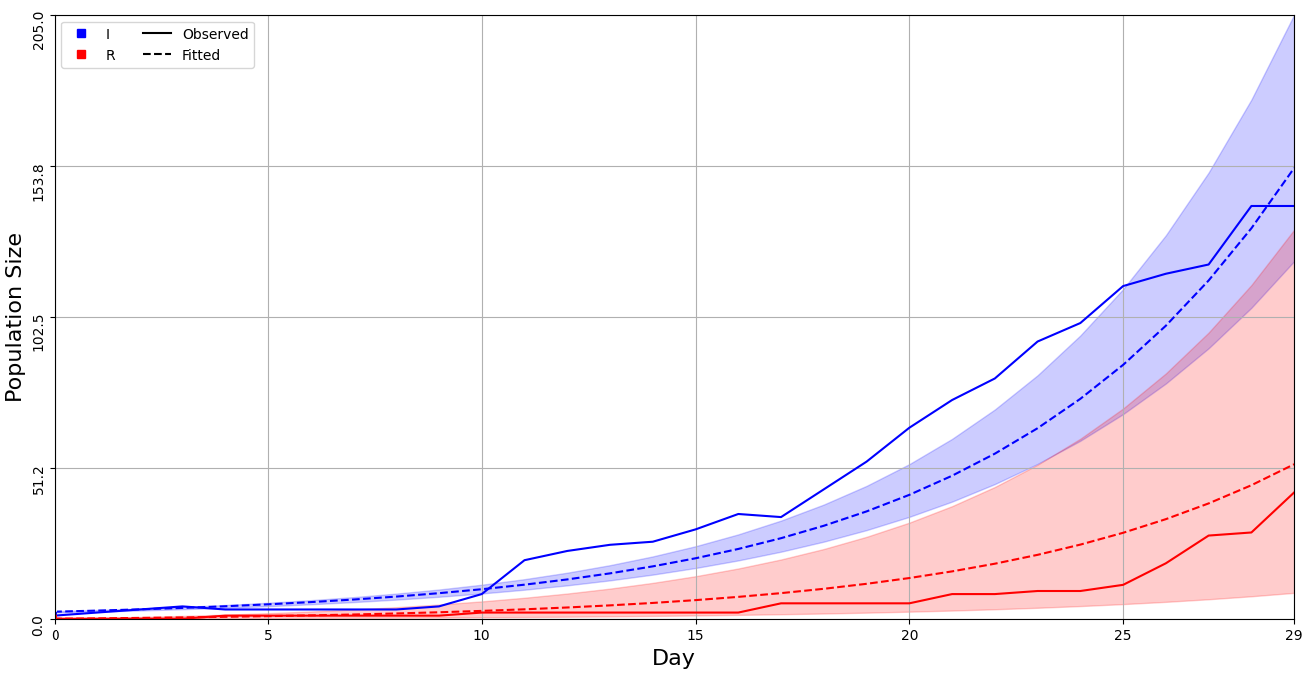
\includegraphics[width=\textwidth]{senegal_semi_auto_adapt_abc_smc_ci.PNG}
        \caption{95\% confidence intervals for population sizes. RSSE=240.}
        \label{fig_senegal_semi_auto_ci}
      \end{subfigure}
    }
    \caption{Estimated posteriors for SIR model parameters and resulting 95\% confidence intervals for the sizes of the infectious (blue) and removed (red) populations for Covid-19 in Senegal between March 2nd 2020 and March 31st 2020 when using Adaptive ABC-SMC with summary statistics generated by Semi-Automatic ABC. 95\% CI for $R_0=[2.547,11.937],\ \beta=[0.163,0.270],\ \gamma=[0.013,0.107]$.}
    \label{}
  \end{figure}


\subsection{More Complex Models}\label{sec_more_complex_models}

  \par Summary statistic methods should perform well in all scenarios where ABC performs well as they are just extensions of ABC.

\newpage
\section{Conclusion}

  \par Selection methods work
  \par Different methods better suited to different problems (2-ME for specific problems and SA-ABC for more general)

\subsection{Future Areas of Research}

  % NOTE alternative to ABC (e.g. indirect inference, Gourieroux and Ronchetti, 1993)

% bibliography
\newpage
\setcounter{page}{1}
\pagenumbering{roman}
\bibliographystyle{royal}
\bibliography{References}

\end{document}
